%&preformat-disser
\RequirePackage[l2tabu,orthodox]{nag} % Раскомментировав, можно в логе получать рекомендации относительно правильного использования пакетов и предупреждения об устаревших и нерекомендуемых пакетах
% Формат А4, 14pt (ГОСТ Р 7.0.11-2011, 5.3.6)
\documentclass[a4paper,14pt,oneside,openany]{memoir}

%% Режим черновика
\makeatletter
\@ifundefined{c@draft}{
  \newcounter{draft}
  \setcounter{draft}{1}  % 0 --- чистовик (максимальное соблюдение ГОСТ)
                         % 1 --- черновик (отклонения от ГОСТ, но быстрая сборка итоговых PDF)
}{}
\makeatother

%% Библиография

%% Внимание! При использовании bibtex8 необходимо удалить все
%% цитирования из  ../common/characteristic.tex
\newcounter{bibliosel}
\setcounter{bibliosel}{1}           % 0 --- встроенная реализация с загрузкой файла через движок bibtex8; 1 --- реализация пакетом biblatex через движок biber
               % общие настройки шаблона
%%% Проверка используемого TeX-движка %%%
\RequirePackage{ifxetex, ifluatex}
\newif\ifxetexorluatex   % определяем новый условный оператор (http://tex.stackexchange.com/a/47579)
\ifxetex
    \xetexorluatextrue
\else
    \ifluatex
        \xetexorluatextrue
    \else
        \xetexorluatexfalse
    \fi
\fi

\RequirePackage{etoolbox}[2015/08/02]               % Для продвинутой проверки разных условий

%%% Поля и разметка страницы %%%
\usepackage{pdflscape}                              % Для включения альбомных страниц
\usepackage{geometry}                               % Для последующего задания полей

%%% Математические пакеты %%%
\usepackage{amsthm,amsfonts,amsmath,amssymb,amscd}  % Математические дополнения от AMS
\usepackage{mathtools}                              % Добавляет окружение multlined

%%%% Установки для размера шрифта 14 pt %%%%
%% Формирование переменных и констант для сравнения (один раз для всех подключаемых файлов)%%
%% должно располагаться до вызова пакета fontspec или polyglossia, потому что они сбивают его работу
\newlength{\curtextsize}
\newlength{\bigtextsize}
\setlength{\bigtextsize}{13.9pt}

\makeatletter
%\show\f@size                                       % неплохо для отслеживания, но вызывает стопорение процесса, если документ компилируется без команды  -interaction=nonstopmode 
\setlength{\curtextsize}{\f@size pt}
\makeatother

%%% Кодировки и шрифты %%%
\ifxetexorluatex
    \usepackage{polyglossia}[2014/05/21]            % Поддержка многоязычности (fontspec подгружается автоматически)
\else
   %%% Решение проблемы копирования текста в буфер кракозябрами
%    \input glyphtounicode.tex
%    \input glyphtounicode-cmr.tex %from pdfx package
%    \pdfgentounicode=1
    \usepackage{cmap}                               % Улучшенный поиск русских слов в полученном pdf-файле
    \defaulthyphenchar=127                          % Если стоит до fontenc, то переносы не впишутся в выделяемый текст при копировании его в буфер обмена
    \usepackage[T2A]{fontenc}                       % Поддержка русских букв
    \usepackage[utf8]{inputenc}[2014/04/30]         % Кодировка utf8
    \usepackage[english, russian]{babel}[2014/03/24]% Языки: русский, английский
    \IfFileExists{pscyr.sty}{\usepackage{pscyr}}{}  % Красивые русские шрифты
\fi

%%% Оформление абзацев %%%
\usepackage{indentfirst}                            % Красная строка

%%% Цвета %%%
\usepackage[dvipsnames,usenames]{color}
\usepackage{colortbl}
%\usepackage[dvipsnames, table, hyperref, cmyk]{xcolor} % Вероятно, более новый вариант, вместо предыдущих двух строк. Конвертация всех цветов в cmyk заложена как удовлетворение возможного требования типографий. Возможно конвертирование и в rgb.

%%% Таблицы %%%
\usepackage{longtable,ltcaption}                    % Длинные таблицы
\usepackage{multirow,makecell}                      % Улучшенное форматирование таблиц

%%% Общее форматирование
\usepackage{soulutf8}                               % Поддержка переносоустойчивых подчёркиваний и зачёркиваний
\usepackage{icomma}                                 % Запятая в десятичных дробях


%%% Гиперссылки %%%
\usepackage{hyperref}[2012/11/06]

%%% Изображения %%%
\usepackage{graphicx}[2014/04/25]                   % Подключаем пакет работы с графикой

%%% Списки %%%
\usepackage{enumitem}

%%% Счётчики %%%
\usepackage[figure,table]{totalcount}               % Счётчик рисунков и таблиц
\usepackage{totcount}                               % Пакет создания счётчиков на основе последнего номера подсчитываемого элемента (может требовать дважды компилировать документ)
\usepackage{totpages}                               % Счётчик страниц, совместимый с hyperref (ссылается на номер последней страницы). Желательно ставить последним пакетом в преамбуле

%%% Продвинутое управление групповыми ссылками (пока только формулами) %%%
\ifxetexorluatex
    \usepackage{cleveref}                           % cleveref корректно считывает язык из настроек polyglossia
\else
    \usepackage[russian]{cleveref}                  % cleveref имеет сложности со считыванием языка из babel. Такое решение русификации вывода выбрано вместо определения в documentclass из опасности что-то лишнее передать во все остальные пакеты, включая библиографию.
\fi
\creflabelformat{equation}{#2#1#3}                  % Формат по умолчанию ставил круглые скобки вокруг каждого номера ссылки, теперь просто номера ссылок без какого-либо дополнительного оформления


\ifnumequal{\value{draft}}{1}{% Черновик
    \usepackage[firstpage]{draftwatermark}
    \SetWatermarkText{DRAFT}
    \SetWatermarkFontSize{14pt}
    \SetWatermarkScale{15}
    \SetWatermarkAngle{45}
}{}

  % Пакеты общие для диссертации и автореферата
%%% Прикладные пакеты %%% 
%\usepackage{calc}               % Пакет для расчётов параметров, например длины

%%% Для добавления Стр. над номерами страниц в оглавлении
%%% http://tex.stackexchange.com/a/306950
\usepackage{afterpage}
         % Пакеты для диссертации
\usepackage{tabu, tabulary}  %таблицы с автоматически подбирающейся шириной столбцов
\usepackage{fr-longtable}    %ради \endlasthead

% Листинги с исходным кодом программ
\usepackage{fancyvrb}
\usepackage{listings}
\lccode`\~=0\relax %Без этого хака из-за особенностей пакета listings перестают работать конструкции с \MakeLowercase и т. п. в (xe|lua)latex

% Русская традиция начертания греческих букв
\usepackage{upgreek} % прямые греческие ради русской традиции

% Микротипографика
%\ifnumequal{\value{draft}}{0}{% Только если у нас режим чистовика
%    \usepackage[final]{microtype}[2016/05/14] % улучшает представление букв и слов в строках, может помочь при наличии отдельно висящих слов
%}{}

% Отметка о версии черновика на каждой странице
% Чтобы работало надо в своей локальной копии по инструкции
% https://www.ctan.org/pkg/gitinfo2 создать небходимые файлы в папке
% ./git/hooks
% If you’re familiar with tweaking git, you can probably work it out for
% yourself. If not, I suggest you follow these steps:
% 1. First, you need a git repository and working tree. For this example,
% let’s suppose that the root of the working tree is in ~/compsci
% 2. Copy the file post-xxx-sample.txt (which is in the same folder of
% your TEX distribution as this pdf) into the git hooks directory in your
% working copy. In our example case, you should end up with a file called
% ~/compsci/.git/hooks/post-checkout
% 3. If you’re using a unix-like system, don’t forget to make the file executable.
% Just how you do this is outside the scope of this manual, but one
% possible way is with commands such as this:
% chmod g+x post-checkout.
% 4. Test your setup with “git checkout master” (or another suitable branch
% name). This should generate copies of gitHeadInfo.gin in the directories
% you intended.
% 5. Now make two more copies of this file in the same directory (hooks),
% calling them post-commit and post-merge, and you’re done. As before,
% users of unix-like systems should ensure these files are marked as
% executable.
\ifnumequal{\value{draft}}{1}{% Черновик
   \IfFileExists{.git/gitHeadInfo.gin}{                                        
      \usepackage[mark,pcount]{gitinfo2}
      \renewcommand{\gitMark}{rev.\gitAbbrevHash\quad\gitCommitterEmail\quad\gitAuthorIsoDate}
      \renewcommand{\gitMarkFormat}{\color{Gray}\small\bfseries}
   }{}
}{}        % Пакеты для специфических пользовательских задач

%%%%%%%%%%%%%%%%%%%%%%%%%%%%%%%%%%%%%%%%%%%%%%%%%%%%%%
%%%% Файл упрощённых настроек шаблона диссертации %%%%
%%%%%%%%%%%%%%%%%%%%%%%%%%%%%%%%%%%%%%%%%%%%%%%%%%%%%%

%%% Инициализирование переменных, не трогать!  %%%
\newcounter{intvl}
\newcounter{otstup}
\newcounter{contnumeq}
\newcounter{contnumfig}
\newcounter{contnumtab}
\newcounter{pgnum}
\newcounter{chapstyle}
\newcounter{headingdelim}
\newcounter{headingalign}
\newcounter{headingsize}
\newcounter{tabcap}
\newcounter{tablaba}
\newcounter{tabtita}
%%%%%%%%%%%%%%%%%%%%%%%%%%%%%%%%%%%%%%%%%%%%%%%%%%

%%% Область упрощённого управления оформлением %%%

%% Интервал между заголовками и между заголовком и текстом
% Заголовки отделяют от текста сверху и снизу тремя интервалами (ГОСТ Р 7.0.11-2011, 5.3.5)
\setcounter{intvl}{3}               % Коэффициент кратности к размеру шрифта

%% Отступы у заголовков в тексте
\setcounter{otstup}{0}              % 0 --- без отступа; 1 --- абзацный отступ

%% Нумерация формул, таблиц и рисунков
\setcounter{contnumeq}{0}           % Нумерация формул: 0 --- пораздельно (во введении подряд, без номера раздела); 1 --- сквозная нумерация по всей диссертации
\setcounter{contnumfig}{0}          % Нумерация рисунков: 0 --- пораздельно (во введении подряд, без номера раздела); 1 --- сквозная нумерация по всей диссертации
\setcounter{contnumtab}{1}          % Нумерация таблиц: 0 --- пораздельно (во введении подряд, без номера раздела); 1 --- сквозная нумерация по всей диссертации

%% Оглавление
\setcounter{pgnum}{0}               % 0 --- номера страниц никак не обозначены; 1 --- Стр. над номерами страниц (дважды компилировать после изменения)
\settocdepth{subsection}            % до какого уровня подразделов выносить в оглавление
\setsecnumdepth{subsection}         % до какого уровня нумеровать подразделы


%% Текст и форматирование заголовков
\setcounter{chapstyle}{1}           % 0 --- разделы только под номером; 1 --- разделы с названием "Глава" перед номером
\setcounter{headingdelim}{1}        % 0 --- номер отделен пропуском в 1em или \quad; 1 --- номера разделов и приложений отделены точкой с пробелом, подразделы пропуском без точки; 2 --- номера разделов, подразделов и приложений отделены точкой с пробелом.

%% Выравнивание заголовков в тексте
\setcounter{headingalign}{0}        % 0 --- по центру; 1 --- по левому краю

%% Размеры заголовков в тексте
\setcounter{headingsize}{0}         % 0 --- по ГОСТ, все всегда 14 пт; 1 --- пропорционально изменяющийся размер в зависимости от базового шрифта

%% Подпись таблиц
\setcounter{tabcap}{0}              % 0 --- по ГОСТ, номер таблицы и название разделены тире, выровнены по левому краю, при необходимости на нескольких строках; 1 --- подпись таблицы не по ГОСТ, на двух и более строках, дальнейшие настройки: 
%Выравнивание первой строки, с подписью и номером
\setcounter{tablaba}{2}             % 0 --- по левому краю; 1 --- по центру; 2 --- по правому краю
%Выравнивание строк с самим названием таблицы
\setcounter{tabtita}{1}             % 0 --- по левому краю; 1 --- по центру; 2 --- по правому краю
%Разделитель записи «Таблица #» и названия таблицы
\newcommand{\tablabelsep}{ }

%% Подпись рисунков
%Разделитель записи «Рисунок #» и названия рисунка
\newcommand{\figlabelsep}{~--- } % (ГОСТ 2.105, 4.3.1)

%%% Цвета гиперссылок %%%
% Latex color definitions: http://latexcolor.com/
\definecolor{linkcolor}{rgb}{0.9,0,0}
\definecolor{citecolor}{rgb}{0,0.6,0}
\definecolor{urlcolor}{rgb}{0,0,1}
%\definecolor{linkcolor}{rgb}{0,0,0} %black
%\definecolor{citecolor}{rgb}{0,0,0} %black
%\definecolor{urlcolor}{rgb}{0,0,0} %black               % Упрощённые настройки шаблона

%%% Переопределение именований, чтобы можно было и в преамбуле использовать %%%
\renewcommand{\chaptername}{Глава}
\renewcommand{\appendixname}{Приложение} % (ГОСТ Р 7.0.11-2011, 5.7)
       % Переопределение именований, чтобы можно было и в преамбуле использовать
% Новые переменные, которые могут использоваться во всём проекте
% ГОСТ 7.0.11-2011
% 9.2 Оформление текста автореферата диссертации
% 9.2.1 Общая характеристика работы включает в себя следующие основные структурные
% элементы:
% актуальность темы исследования;
\newcommand{\actualityTXT}{Актуальность темы.}
% степень ее разработанности;
\newcommand{\progressTXT}{Степень разработанности темы.}
% цели и задачи;
\newcommand{\aimTXT}{Целью}
\newcommand{\tasksTXT}{задачи}
% научную новизну;
\newcommand{\noveltyTXT}{Научная новизна:}
% теоретическую и практическую значимость работы;
%\newcommand{\influenceTXT}{Теоретическая и практическая значимость}
% или чаще используют просто
\newcommand{\influenceTXT}{Практическая значимость}
% методологию и методы исследования;
\newcommand{\methodsTXT}{Mетодология и методы исследования.}
% положения, выносимые на защиту;
\newcommand{\defpositionsTXT}{Основные положения, выносимые на~защиту:}
% степень достоверности и апробацию результатов.
\newcommand{\reliabilityTXT}{Достоверность}
\newcommand{\probationTXT}{Апробация работы.}

\newcommand{\contributionTXT}{Личный вклад.}
\newcommand{\publicationsTXT}{Публикации.}


\newcommand{\authorbibtitle}{Публикации автора по теме диссертации}
\newcommand{\vakbibtitle}{В изданиях из списка ВАК РФ}
\newcommand{\notvakbibtitle}{В прочих изданиях}
\newcommand{\confbibtitle}{В сборниках трудов конференций}
\newcommand{\fullbibtitle}{Список литературы} % (ГОСТ Р 7.0.11-2011, 4)
  % Новые переменные, которые могут использоваться во всём проекте

%%% Основные сведения %%%
\newcommand{\thesisAuthor}             % Диссертация, ФИО автора
{%
    \texorpdfstring{% \texorpdfstring takes two arguments and uses the first for (La)TeX and the second for pdf
        \todo{Фасахов Роман Равилевич}% так будет отображаться на титульном листе или в тексте, где будет использоваться переменная
    }{%
        Фасахов, Роман Равилевич% эта запись для свойств pdf-файла. В таком виде, если pdf будет обработан программами для сбора библиографических сведений, будет правильно представлена фамилия.
    }%
}
\newcommand{\thesisAuthorShort}        % Диссертация, ФИО автора инициалами
{\todo{Р.Р.~Фасахов}}

%\newcommand{\thesisUdk}                % Диссертация, УДК
%{\todo{xxx.xxx}}
\newcommand{\thesisTitle}              % Диссертация, название
{\texorpdfstring{\todo{\MakeUppercase{Конечно-элементное моделирование и исследование сферического ротора в электростатическом подвесе}}}{Конечно-элементное моделирование и исследование сферического ротора в электростатическом подвесе}}
\newcommand{\thesisSpecialtyNumber}    % Диссертация, специальность, номер
{\texorpdfstring{\todo{15.03.03}}{15.03.03}}
\newcommand{\thesisSpecialtyTitle}     % Диссертация, специальность, название
{\texorpdfstring{\todo{Прикладная механика}}{Прикладная механика}}
\newcommand{\thesisDegree}             % Диссертация, ученая степень
{\todo{кандидата физико-математических наук}}
\newcommand{\thesisDegreeShort}        % Диссертация, ученая степень, краткая запись
{\todo{канд. физ.-мат. наук}}
\newcommand{\thesisCity}               % Диссертация, город написания диссертации
{\todo{Санкт-Петербург}}
\newcommand{\thesisYear}               % Диссертация, год написания диссертации
{\todo{2017}}
\newcommand{\thesisOrganization}       % Диссертация, организация
{\todo{«Санкт-Петербургский политехнический университет Петра Великого»}}
\newcommand{\thesisOrganizationShort}  % Диссертация, краткое название организации для доклада
{\todo{СПбПУ}}

\newcommand{\thesisInOrganization}     % Диссертация, организация в предложном падеже: Работа выполнена в ...
{\todo{Санкт-Петербургском политехническом университете}}

\newcommand{\supervisorFio}            % Научный руководитель, ФИО
{\todo{Попов Иван Алексеевич}}
\newcommand{\supervisorRegalia}        % Научный руководитель, регалии
{\todo{ассистент}}
\newcommand{\supervisorFioShort}       % Научный руководитель, ФИО
{\todo{И.А.~Попов}}
\newcommand{\supervisorRegaliaShort}   % Научный руководитель, регалии
{\todo{асс.}}


\newcommand{\opponentOneFio}           % Оппонент 1, ФИО
{\todo{Фамилия Имя Отчество}}
\newcommand{\opponentOneRegalia}       % Оппонент 1, регалии
{\todo{доктор физико-математических наук, профессор}}
\newcommand{\opponentOneJobPlace}      % Оппонент 1, место работы
{\todo{Не очень длинное название для места работы}}
\newcommand{\opponentOneJobPost}       % Оппонент 1, должность
{\todo{старший научный сотрудник}}

\newcommand{\opponentTwoFio}           % Оппонент 2, ФИО
{\todo{Фамилия Имя Отчество}}
\newcommand{\opponentTwoRegalia}       % Оппонент 2, регалии
{\todo{кандидат физико-математических наук}}
\newcommand{\opponentTwoJobPlace}      % Оппонент 2, место работы
{\todo{Основное место работы c длинным длинным длинным длинным названием}}
\newcommand{\opponentTwoJobPost}       % Оппонент 2, должность
{\todo{старший научный сотрудник}}

\newcommand{\leadingOrganizationTitle} % Ведущая организация, дополнительные строки
{\todo{Федеральное государственное бюджетное образовательное учреждение высшего профессионального образования с~длинным длинным длинным длинным названием}}

\newcommand{\defenseDate}              % Защита, дата
{\todo{21 июня 2017~г.~в~10 часов}}
\newcommand{\defenseCouncilNumber}     % Защита, номер диссертационного совета
{\todo{Д\,123.456.78}}
\newcommand{\defenseCouncilTitle}      % Защита, учреждение диссертационного совета
{\todo{Название учреждения}}
\newcommand{\defenseCouncilAddress}    % Защита, адрес учреждение диссертационного совета
{\todo{Адрес}}
\newcommand{\defenseCouncilPhone}      % Телефон для справок
{\todo{+7~(911)~704-43-44}}

\newcommand{\defenseSecretaryFio}      % Секретарь диссертационного совета, ФИО
{\todo{Фамилия Имя Отчество}}
\newcommand{\defenseSecretaryRegalia}  % Секретарь диссертационного совета, регалии
{\todo{д-р~физ.-мат. наук}}            % Для сокращений есть ГОСТы, например: ГОСТ Р 7.0.12-2011 + http://base.garant.ru/179724/#block_30000

\newcommand{\synopsisLibrary}          % Автореферат, название библиотеки
{\todo{Название библиотеки}}
\newcommand{\synopsisDate}             % Автореферат, дата рассылки
{\todo{DD mmmmmmmm YYYY года}}

% To avoid conflict with beamer class use \providecommand
\providecommand{\keywords}%            % Ключевые слова для метаданных PDF диссертации и автореферата
{}      % Основные сведения
%%% Кодировки и шрифты %%%
\ifxetexorluatex
    \setmainlanguage[babelshorthands=true]{russian}  % Язык по-умолчанию русский с поддержкой приятных команд пакета babel
    \setotherlanguage{english}                       % Дополнительный язык = английский (в американской вариации по-умолчанию)
    \setmonofont{Courier New}                        % моноширинный шрифт
    \newfontfamily\cyrillicfonttt{Courier New}       % моноширинный шрифт для кириллицы
    \defaultfontfeatures{Ligatures=TeX}              % стандартные лигатуры TeX, замены нескольких дефисов на тире и т. п. Настройки моноширинного шрифта должны идти до этой строки, чтобы при врезках кода программ в коде не применялись лигатуры и замены дефисов
    \setmainfont{Times New Roman}                    % Шрифт с засечками
    \newfontfamily\cyrillicfont{Times New Roman}     % Шрифт с засечками для кириллицы
    \setsansfont{Arial}                              % Шрифт без засечек
    \newfontfamily\cyrillicfontsf{Arial}             % Шрифт без засечек для кириллицы
\else
    \IfFileExists{pscyr.sty}{\renewcommand{\rmdefault}{ftm}}{}
\fi

%%% Подписи %%%
\setlength{\abovecaptionskip}{0pt}   % Отбивка над подписью
\setlength{\belowcaptionskip}{0pt}   % Отбивка под подписью
\captionwidth{\linewidth}
\normalcaptionwidth

%%% Таблицы %%%
\ifnumequal{\value{tabcap}}{0}{%
    \newcommand{\tabcapalign}{\raggedright}  % по левому краю страницы или аналога parbox
    \renewcommand{\tablabelsep}{~--- } % тире как разделитель идентификатора с номером от наименования
    \newcommand{\tabtitalign}{}
}{%
    \ifnumequal{\value{tablaba}}{0}{%
        \newcommand{\tabcapalign}{\raggedright}  % по левому краю страницы или аналога parbox
    }{}

    \ifnumequal{\value{tablaba}}{1}{%
        \newcommand{\tabcapalign}{\centering}    % по центру страницы или аналога parbox
    }{}

    \ifnumequal{\value{tablaba}}{2}{%
        \newcommand{\tabcapalign}{\raggedleft}   % по правому краю страницы или аналога parbox
    }{}

    \ifnumequal{\value{tabtita}}{0}{%
        \newcommand{\tabtitalign}{\par\raggedright}  % по левому краю страницы или аналога parbox
    }{}

    \ifnumequal{\value{tabtita}}{1}{%
        \newcommand{\tabtitalign}{\par\centering}    % по центру страницы или аналога parbox
    }{}

    \ifnumequal{\value{tabtita}}{2}{%
        \newcommand{\tabtitalign}{\par\raggedleft}   % по правому краю страницы или аналога parbox
    }{}
}

\precaption{\tabcapalign} % всегда идет перед подписью или \legend
\captionnamefont{\normalfont\normalsize} % Шрифт надписи «Таблица #»; также определяет шрифт у \legend
\captiondelim{\tablabelsep} % разделитель идентификатора с номером от наименования
\captionstyle[\tabtitalign]{\tabtitalign}
\captiontitlefont{\normalfont\normalsize} % Шрифт с текстом подписи

%%% Рисунки %%%
\setfloatadjustment{figure}{%
    \setlength{\abovecaptionskip}{0pt}   % Отбивка над подписью
    \setlength{\belowcaptionskip}{0pt}   % Отбивка под подписью
    \precaption{} % всегда идет перед подписью или \legend
    \captionnamefont{\normalfont\normalsize} % Шрифт надписи «Рисунок #»; также определяет шрифт у \legend
    \captiondelim{\figlabelsep} % разделитель идентификатора с номером от наименования
    \captionstyle[\centering]{\centering} % Центрирование подписей, заданных командой \caption и \legend
    \captiontitlefont{\normalfont\normalsize} % Шрифт с текстом подписи
    \postcaption{} % всегда идет после подписи или \legend, и с новой строки
}

%%% Подписи подрисунков %%%
\newsubfloat{figure} % Включает возможность использовать подрисунки у окружений figure
\renewcommand{\thesubfigure}{\asbuk{subfigure}}           % Буквенные номера подрисунков
\subcaptionsize{\normalsize} % Шрифт подписи названий подрисунков (не отличается от основного)
\subcaptionlabelfont{\normalfont}
\subcaptionfont{\!\!) \normalfont} % Вот так тут добавили скобку после буквы.
\subcaptionstyle{\centering}
%\subcaptionsize{\fontsize{12pt}{13pt}\selectfont} % объявляем шрифт 12pt для использования в подписях, тут же надо интерлиньяж объявлять, если не наследуется

%%% Настройки гиперссылок %%%
\ifluatex
    \hypersetup{
        unicode,                % Unicode encoded PDF strings
    }
\fi

\hypersetup{
    linktocpage=true,           % ссылки с номера страницы в оглавлении, списке таблиц и списке рисунков
%    linktoc=all,                % both the section and page part are links
%    pdfpagelabels=false,        % set PDF page labels (true|false)
    plainpages=false,           % Forces page anchors to be named by the Arabic form  of the page number, rather than the formatted form
    colorlinks,                 % ссылки отображаются раскрашенным текстом, а не раскрашенным прямоугольником, вокруг текста
    linkcolor={black},      % цвет ссылок типа ref, eqref и подобных
    citecolor={black},      % цвет ссылок-цитат
    urlcolor={black},        % цвет гиперссылок
%    hidelinks,                  % Hide links (removing color and border)
    pdftitle={\thesisTitle},    % Заголовок
    pdfauthor={\thesisAuthor},  % Автор
    pdfsubject={\thesisSpecialtyNumber\ \thesisSpecialtyTitle},      % Тема
%    pdfcreator={Создатель},     % Создатель, Приложение
%    pdfproducer={Производитель},% Производитель, Производитель PDF
    pdfkeywords={\keywords},    % Ключевые слова
    pdflang={ru},
}
\ifnumequal{\value{draft}}{1}{% Черновик
    \hypersetup{
        draft,
    }
}{}

%%% Шаблон %%%
\DeclareRobustCommand{\todo}{\textcolor{black}}       % решаем проблему превращения названия цвета в результате \MakeUppercase, http://tex.stackexchange.com/a/187930/79756 , \DeclareRobustCommand protects \todo from expanding inside \MakeUppercase
\AtBeginDocument{%
    \setlength{\parindent}{2.5em}                   % Абзацный отступ. Должен быть одинаковым по всему тексту и равен пяти знакам (ГОСТ Р 7.0.11-2011, 5.3.7).
}

%%% Списки %%%
% Используем короткое тире (endash) для ненумерованных списков (ГОСТ 2.105-95, пункт 4.1.7, требует дефиса, но так лучше смотрится)
\renewcommand{\labelitemi}{\normalfont\bfseries{--}}

% Перечисление строчными буквами латинского алфавита (ГОСТ 2.105-95, 4.1.7)
%\renewcommand{\theenumi}{\alph{enumi}}
%\renewcommand{\labelenumi}{\theenumi)} 

% Перечисление строчными буквами русского алфавита (ГОСТ 2.105-95, 4.1.7)
\makeatletter
\AddEnumerateCounter{\asbuk}{\russian@alph}{щ}      % Управляем списками/перечислениями через пакет enumitem, а он 'не знает' про asbuk, потому 'учим' его
\makeatother
%\renewcommand{\theenumi}{\asbuk{enumi}} %первый уровень нумерации
%\renewcommand{\labelenumi}{\theenumi)} %первый уровень нумерации 
\renewcommand{\theenumii}{\asbuk{enumii}} %второй уровень нумерации
\renewcommand{\labelenumii}{\theenumii)} %второй уровень нумерации 
\renewcommand{\theenumiii}{\arabic{enumiii}} %третий уровень нумерации
\renewcommand{\labelenumiii}{\theenumiii)} %третий уровень нумерации 

\setlist{nosep,%                                    % Единый стиль для всех списков (пакет enumitem), без дополнительных интервалов.
    labelindent=\parindent,leftmargin=*%            % Каждый пункт, подпункт и перечисление записывают с абзацного отступа (ГОСТ 2.105-95, 4.1.8)
}
    % Стили общие для диссертации и автореферата
%%% Изображения %%%
\graphicspath{{images/}{Dissertation/images/}}         % Пути к изображениям

%%% Макет страницы %%%
% Выставляем значения полей (ГОСТ 7.0.11-2011, 5.3.7)
\geometry{a4paper,top=2cm,bottom=2cm,left=2.5cm,right=1cm,nofoot,nomarginpar} %,showframe
\setlength{\topskip}{0pt}   %размер дополнительного верхнего поля
\setlength{\footskip}{12.3pt} % снимет warning, согласно https://tex.stackexchange.com/a/334346

%%% Интервалы %%%
%% По ГОСТ Р 7.0.11-2011, пункту 5.3.6 требуется полуторный интервал
%% Реализация средствами класса (на основе setspace) ближе к типографской классике.
%% И правит сразу и в таблицах (если со звёздочкой) 
%\DoubleSpacing*     % Двойной интервал
\OnehalfSpacing*    % Полуторный интервал
%\setSpacing{1.42}   % Полуторный интервал, подобный Ворду (возможно, стоит включать вместе с предыдущей строкой)

%%% Выравнивание и переносы %%%
%% http://tex.stackexchange.com/questions/241343/what-is-the-meaning-of-fussy-sloppy-emergencystretch-tolerance-hbadness
%% http://www.latex-community.org/forum/viewtopic.php?p=70342#p70342
\tolerance 1414
\hbadness 1414
\emergencystretch 1.5em % В случае проблем регулировать в первую очередь
\hfuzz 0.3pt
\vfuzz \hfuzz
%\raggedbottom
%\sloppy                 % Избавляемся от переполнений
\clubpenalty=10000      % Запрещаем разрыв страницы после первой строки абзаца
\widowpenalty=10000     % Запрещаем разрыв страницы после последней строки абзаца

%%% Блок управления параметрами для выравнивания заголовков в тексте %%%
\newlength{\otstuplen}
\setlength{\otstuplen}{\theotstup\parindent}
\ifnumequal{\value{headingalign}}{0}{% выравнивание заголовков в тексте
    \newcommand{\hdngalign}{\centering}                % по центру
    \newcommand{\hdngaligni}{}% по центру
    \setlength{\otstuplen}{0pt}
}{%
    \newcommand{\hdngalign}{}                 % по левому краю
    \newcommand{\hdngaligni}{\hspace{\otstuplen}}      % по левому краю
} % В обоих случаях вроде бы без переноса, как и надо (ГОСТ Р 7.0.11-2011, 5.3.5)

%%% Оглавление %%%
\renewcommand{\cftchapterdotsep}{\cftdotsep}                % отбивка точками до номера страницы начала главы/раздела

%% Переносить слова в заголовке не допускается (ГОСТ Р 7.0.11-2011, 5.3.5). Заголовки в оглавлении должны точно повторять заголовки в тексте (ГОСТ Р 7.0.11-2011, 5.2.3). Прямого указания на запрет переносов в оглавлении нет, но по той же логике невнесения искажений в смысл, лучше в оглавлении не переносить:
\setrmarg{2.55em plus1fil}                             %To have the (sectional) titles in the ToC, etc., typeset ragged right with no hyphenation
\renewcommand{\cftchapterpagefont}{\normalfont}        % нежирные номера страниц у глав в оглавлении
\renewcommand{\cftchapterleader}{\cftdotfill{\cftchapterdotsep}}% нежирные точки до номеров страниц у глав в оглавлении
%\renewcommand{\cftchapterfont}{}                       % нежирные названия глав в оглавлении

\ifnumgreater{\value{headingdelim}}{0}{%
    \renewcommand\cftchapteraftersnum{.\space}       % добавляет точку с пробелом после номера раздела в оглавлении
}{}
\ifnumgreater{\value{headingdelim}}{1}{%
    \renewcommand\cftsectionaftersnum{.\space}       % добавляет точку с пробелом после номера подраздела в оглавлении
    \renewcommand\cftsubsectionaftersnum{.\space}    % добавляет точку с пробелом после номера подподраздела в оглавлении
    \renewcommand\cftsubsubsectionaftersnum{.\space} % добавляет точку с пробелом после номера подподподраздела в оглавлении
    \AtBeginDocument{% без этого polyglossia сама всё переопределяет
        \setsecnumformat{\csname the#1\endcsname.\space}
    }
}{%
    \AtBeginDocument{% без этого polyglossia сама всё переопределяет
        \setsecnumformat{\csname the#1\endcsname\quad}
    }
}

\renewcommand*{\cftappendixname}{\appendixname\space} % Слово Приложение в оглавлении

%%% Колонтитулы %%%
% Порядковый номер страницы печатают на середине верхнего поля страницы (ГОСТ Р 7.0.11-2011, 5.3.8)
\makeevenhead{plain}{}{\thepage}{}
\makeoddhead{plain}{}{\thepage}{}
\makeevenfoot{plain}{}{}{}
\makeoddfoot{plain}{}{}{}
\pagestyle{plain}

%%% добавить Стр. над номерами страниц в оглавлении
%%% http://tex.stackexchange.com/a/306950
\newif\ifendTOC

\newcommand*{\tocheader}{
\ifnumequal{\value{pgnum}}{1}{%
    \ifendTOC\else\hbox to \linewidth%
      {\noindent{}~\hfill{Стр.}}\par%
      \ifnumless{\value{page}}{3}{}{%
        \vspace{0.5\onelineskip}
      }
      \afterpage{\tocheader}
    \fi%
}{}%
}%

%%% Оформление заголовков глав, разделов, подразделов %%%
%% Работа должна быть выполнена ... размером шрифта 12-14 пунктов (ГОСТ Р 7.0.11-2011, 5.3.8). То есть не должно быть надписей шрифтом более 14. Так и поставим.
%% Эти установки будут давать одинаковый результат независимо от выбора базовым шрифтом 12 пт или 14 пт
\newcommand{\basegostsectionfont}{\fontsize{14pt}{16pt}\selectfont\bfseries}

\makechapterstyle{thesisgost}{%
    \chapterstyle{default}
    \setlength{\beforechapskip}{0pt}
    \setlength{\midchapskip}{0pt}
    \setlength{\afterchapskip}{\theintvl\curtextsize}
    \renewcommand*{\chapnamefont}{\basegostsectionfont}
    \renewcommand*{\chapnumfont}{\basegostsectionfont}
    \renewcommand*{\chaptitlefont}{\basegostsectionfont}
    \renewcommand*{\chapterheadstart}{}
    \ifnumgreater{\value{headingdelim}}{0}{%
        \renewcommand*{\afterchapternum}{.\space}   % добавляет точку с пробелом после номера раздела
    }{%
        \renewcommand*{\afterchapternum}{\quad}     % добавляет \quad после номера раздела
    }
    \renewcommand*{\printchapternum}{\hdngaligni\hdngalign\chapnumfont \thechapter}
    \renewcommand*{\printchaptername}{}
    \renewcommand*{\printchapternonum}{\hdngaligni\hdngalign}
}

\makeatletter
\makechapterstyle{thesisgostchapname}{%
    \chapterstyle{thesisgost}
    \renewcommand*{\printchapternum}{\chapnumfont \thechapter}
    \renewcommand*{\printchaptername}{\hdngaligni\hdngalign\chapnamefont \@chapapp} %
}
\makeatother

\chapterstyle{thesisgost}

\setsecheadstyle{\basegostsectionfont\hdngalign}
\setsecindent{\otstuplen}

\setsubsecheadstyle{\basegostsectionfont\hdngalign}
\setsubsecindent{\otstuplen}

\setsubsubsecheadstyle{\basegostsectionfont\hdngalign}
\setsubsubsecindent{\otstuplen}

\sethangfrom{\noindent #1} %все заголовки подразделов центрируются с учетом номера, как block 

\ifnumequal{\value{chapstyle}}{1}{%
    \chapterstyle{thesisgostchapname}
    \renewcommand*{\cftchaptername}{\chaptername\space} % будет вписано слово Глава перед каждым номером раздела в оглавлении
}{}%

%%% Интервалы между заголовками
\setbeforesecskip{\theintvl\curtextsize}% Заголовки отделяют от текста сверху и снизу тремя интервалами (ГОСТ Р 7.0.11-2011, 5.3.5).
\setaftersecskip{\theintvl\curtextsize}
\setbeforesubsecskip{\theintvl\curtextsize}
\setaftersubsecskip{\theintvl\curtextsize}
\setbeforesubsubsecskip{\theintvl\curtextsize}
\setaftersubsubsecskip{\theintvl\curtextsize}

%%% Блок дополнительного управления размерами заголовков
\ifnumequal{\value{headingsize}}{1}{% Пропорциональные заголовки и базовый шрифт 14 пт
    \renewcommand{\basegostsectionfont}{\large\bfseries}
    \renewcommand*{\chapnamefont}{\Large\bfseries}
    \renewcommand*{\chapnumfont}{\Large\bfseries}
    \renewcommand*{\chaptitlefont}{\Large\bfseries}
}{}

%%% Счётчики %%%

%% Упрощённые настройки шаблона диссертации: нумерация формул, таблиц, рисунков
\ifnumequal{\value{contnumeq}}{1}{%
    \counterwithout{equation}{chapter} % Убираем связанность номера формулы с номером главы/раздела
}{}
\ifnumequal{\value{contnumfig}}{1}{%
    \counterwithout{figure}{chapter}   % Убираем связанность номера рисунка с номером главы/раздела
}{}
\ifnumequal{\value{contnumtab}}{1}{%
    \counterwithout{table}{chapter}    % Убираем связанность номера таблицы с номером главы/раздела
}{}


%%http://www.linux.org.ru/forum/general/6993203#comment-6994589 (используется totcount)
\makeatletter
\def\formbytotal#1#2#3#4#5{%
    \newcount\@c
    \@c\totvalue{#1}\relax
    \newcount\@last
    \newcount\@pnul
    \@last\@c\relax
    \divide\@last 10
    \@pnul\@last\relax
    \divide\@pnul 10
    \multiply\@pnul-10
    \advance\@pnul\@last
    \multiply\@last-10
    \advance\@last\@c
    \total{#1}~#2%
    \ifnum\@pnul=1#5\else%
    \ifcase\@last#5\or#3\or#4\or#4\or#4\else#5\fi
    \fi
}
\makeatother

\AtBeginDocument{
%% регистрируем счётчики в системе totcounter
    \regtotcounter{totalcount@figure}
    \regtotcounter{totalcount@table}       % Если иным способом поставить в преамбуле то ошибка в числе таблиц
    \regtotcounter{TotPages}               % Если иным способом поставить в преамбуле то ошибка в числе страниц
}

%%% Правильная нумерация приложений %%%
%% По ГОСТ 2.105, п. 4.3.8 Приложения обозначают заглавными буквами русского алфавита,
%% начиная с А, за исключением букв Ё, З, Й, О, Ч, Ь, Ы, Ъ.
%% Здесь также переделаны все нумерации русскими буквами.
\ifxetexorluatex
    \makeatletter
    \def\russian@Alph#1{\ifcase#1\or
       А\or Б\or В\or Г\or Д\or Е\or Ж\or
       И\or К\or Л\or М\or Н\or
       П\or Р\or С\or Т\or У\or Ф\or Х\or
       Ц\or Ш\or Щ\or Э\or Ю\or Я\else\xpg@ill@value{#1}{russian@Alph}\fi}
    \def\russian@alph#1{\ifcase#1\or
       а\or б\or в\or г\or д\or е\or ж\or
       и\or к\or л\or м\or н\or
       п\or р\or с\or т\or у\or ф\or х\or
       ц\or ш\or щ\or э\or ю\or я\else\xpg@ill@value{#1}{russian@alph}\fi}
    \makeatother
\else
    \makeatletter
    \if@uni@ode
      \def\russian@Alph#1{\ifcase#1\or
        А\or Б\or В\or Г\or Д\or Е\or Ж\or
        И\or К\or Л\or М\or Н\or
        П\or Р\or С\or Т\or У\or Ф\or Х\or
        Ц\or Ш\or Щ\or Э\or Ю\or Я\else\@ctrerr\fi}
    \else
      \def\russian@Alph#1{\ifcase#1\or
        \CYRA\or\CYRB\or\CYRV\or\CYRG\or\CYRD\or\CYRE\or\CYRZH\or
        \CYRI\or\CYRK\or\CYRL\or\CYRM\or\CYRN\or
        \CYRP\or\CYRR\or\CYRS\or\CYRT\or\CYRU\or\CYRF\or\CYRH\or
        \CYRC\or\CYRSH\or\CYRSHCH\or\CYREREV\or\CYRYU\or
        \CYRYA\else\@ctrerr\fi}
    \fi
    \if@uni@ode
      \def\russian@alph#1{\ifcase#1\or
        а\or б\or в\or г\or д\or е\or ж\or
        и\or к\or л\or м\or н\or
        п\or р\or с\or т\or у\or ф\or х\or
        ц\or ш\or щ\or э\or ю\or я\else\@ctrerr\fi}
    \else
      \def\russian@alph#1{\ifcase#1\or
        \cyra\or\cyrb\or\cyrv\or\cyrg\or\cyrd\or\cyre\or\cyrzh\or
        \cyri\or\cyrk\or\cyrl\or\cyrm\or\cyrn\or
        \cyrp\or\cyrr\or\cyrs\or\cyrt\or\cyru\or\cyrf\or\cyrh\or
        \cyrc\or\cyrsh\or\cyrshch\or\cyrerev\or\cyryu\or
        \cyrya\else\@ctrerr\fi}
    \fi
    \makeatother
\fi           % Стили для диссертации
% для вертикального центрирования ячеек в tabulary
\def\zz{\ifx\[$\else\aftergroup\zzz\fi}
%$ \] % <-- чиним подсветку синтаксиса в некоторых редакторах
\def\zzz{\setbox0\lastbox
\dimen0\dimexpr\extrarowheight + \ht0-\dp0\relax
\setbox0\hbox{\raise-.5\dimen0\box0}%
\ht0=\dimexpr\ht0+\extrarowheight\relax
\dp0=\dimexpr\dp0+\extrarowheight\relax 
\box0
}



\lstdefinelanguage{Renhanced}%
{keywords={abbreviate,abline,abs,acos,acosh,action,add1,add,%
        aggregate,alias,Alias,alist,all,anova,any,aov,aperm,append,apply,%
        approx,approxfun,apropos,Arg,args,array,arrows,as,asin,asinh,%
        atan,atan2,atanh,attach,attr,attributes,autoload,autoloader,ave,%
        axis,backsolve,barplot,basename,besselI,besselJ,besselK,besselY,%
        beta,binomial,body,box,boxplot,break,browser,bug,builtins,bxp,by,%
        c,C,call,Call,case,cat,category,cbind,ceiling,character,char,%
        charmatch,check,chol,chol2inv,choose,chull,class,close,cm,codes,%
        coef,coefficients,co,col,colnames,colors,colours,commandArgs,%
        comment,complete,complex,conflicts,Conj,contents,contour,%
        contrasts,contr,control,helmert,contrib,convolve,cooks,coords,%
        distance,coplot,cor,cos,cosh,count,fields,cov,covratio,wt,CRAN,%
        create,crossprod,cummax,cummin,cumprod,cumsum,curve,cut,cycle,D,%
        data,dataentry,date,dbeta,dbinom,dcauchy,dchisq,de,debug,%
        debugger,Defunct,default,delay,delete,deltat,demo,de,density,%
        deparse,dependencies,Deprecated,deriv,description,detach,%
        dev2bitmap,dev,cur,deviance,off,prev,,dexp,df,dfbetas,dffits,%
        dgamma,dgeom,dget,dhyper,diag,diff,digamma,dim,dimnames,dir,%
        dirname,dlnorm,dlogis,dnbinom,dnchisq,dnorm,do,dotplot,double,%
        download,dpois,dput,drop,drop1,dsignrank,dt,dummy,dump,dunif,%
        duplicated,dweibull,dwilcox,dyn,edit,eff,effects,eigen,else,%
        emacs,end,environment,env,erase,eval,equal,evalq,example,exists,%
        exit,exp,expand,expression,External,extract,extractAIC,factor,%
        fail,family,fft,file,filled,find,fitted,fivenum,fix,floor,for,%
        For,formals,format,formatC,formula,Fortran,forwardsolve,frame,%
        frequency,ftable,ftable2table,function,gamma,Gamma,gammaCody,%
        gaussian,gc,gcinfo,gctorture,get,getenv,geterrmessage,getOption,%
        getwd,gl,glm,globalenv,gnome,GNOME,graphics,gray,grep,grey,grid,%
        gsub,hasTsp,hat,heat,help,hist,home,hsv,httpclient,I,identify,if,%
        ifelse,Im,image,\%in\%,index,influence,measures,inherits,install,%
        installed,integer,interaction,interactive,Internal,intersect,%
        inverse,invisible,IQR,is,jitter,kappa,kronecker,labels,lapply,%
        layout,lbeta,lchoose,lcm,legend,length,levels,lgamma,library,%
        licence,license,lines,list,lm,load,local,locator,log,log10,log1p,%
        log2,logical,loglin,lower,lowess,ls,lsfit,lsf,ls,machine,Machine,%
        mad,mahalanobis,make,link,margin,match,Math,matlines,mat,matplot,%
        matpoints,matrix,max,mean,median,memory,menu,merge,methods,min,%
        missing,Mod,mode,model,response,mosaicplot,mtext,mvfft,na,nan,%
        names,omit,nargs,nchar,ncol,NCOL,new,next,NextMethod,nextn,%
        nlevels,nlm,noquote,NotYetImplemented,NotYetUsed,nrow,NROW,null,%
        numeric,\%o\%,objects,offset,old,on,Ops,optim,optimise,optimize,%
        options,or,order,ordered,outer,package,packages,page,pairlist,%
        pairs,palette,panel,par,parent,parse,paste,path,pbeta,pbinom,%
        pcauchy,pchisq,pentagamma,persp,pexp,pf,pgamma,pgeom,phyper,pico,%
        pictex,piechart,Platform,plnorm,plogis,plot,pmatch,pmax,pmin,%
        pnbinom,pnchisq,pnorm,points,poisson,poly,polygon,polyroot,pos,%
        postscript,power,ppoints,ppois,predict,preplot,pretty,Primitive,%
        print,prmatrix,proc,prod,profile,proj,prompt,prop,provide,%
        psignrank,ps,pt,ptukey,punif,pweibull,pwilcox,q,qbeta,qbinom,%
        qcauchy,qchisq,qexp,qf,qgamma,qgeom,qhyper,qlnorm,qlogis,qnbinom,%
        qnchisq,qnorm,qpois,qqline,qqnorm,qqplot,qr,Q,qty,qy,qsignrank,%
        qt,qtukey,quantile,quasi,quit,qunif,quote,qweibull,qwilcox,%
        rainbow,range,rank,rbeta,rbind,rbinom,rcauchy,rchisq,Re,read,csv,%
        csv2,fwf,readline,socket,real,Recall,rect,reformulate,regexpr,%
        relevel,remove,rep,repeat,replace,replications,report,require,%
        resid,residuals,restart,return,rev,rexp,rf,rgamma,rgb,rgeom,R,%
        rhyper,rle,rlnorm,rlogis,rm,rnbinom,RNGkind,rnorm,round,row,%
        rownames,rowsum,rpois,rsignrank,rstandard,rstudent,rt,rug,runif,%
        rweibull,rwilcox,sample,sapply,save,scale,scan,scan,screen,sd,se,%
        search,searchpaths,segments,seq,sequence,setdiff,setequal,set,%
        setwd,show,sign,signif,sin,single,sinh,sink,solve,sort,source,%
        spline,splinefun,split,sqrt,stars,start,stat,stem,step,stop,%
        storage,strstrheight,stripplot,strsplit,structure,strwidth,sub,%
        subset,substitute,substr,substring,sum,summary,sunflowerplot,svd,%
        sweep,switch,symbol,symbols,symnum,sys,status,system,t,table,%
        tabulate,tan,tanh,tapply,tempfile,terms,terrain,tetragamma,text,%
        time,title,topo,trace,traceback,transform,tri,trigamma,trunc,try,%
        ts,tsp,typeof,unclass,undebug,undoc,union,unique,uniroot,unix,%
        unlink,unlist,unname,untrace,update,upper,url,UseMethod,var,%
        variable,vector,Version,vi,warning,warnings,weighted,weights,%
        which,while,window,write,\%x\%,x11,X11,xedit,xemacs,xinch,xor,%
        xpdrows,xy,xyinch,yinch,zapsmall,zip},%
    otherkeywords={!,!=,~,$,*,\%,\&,\%/\%,\%*\%,\%\%,<-,<<-},%$
    alsoother={._$},%$
    sensitive,%
    morecomment=[l]\#,%
    morestring=[d]",%
    morestring=[d]'% 2001 Robert Denham
}%

%решаем проблему с кириллицей в комментариях (в pdflatex) https://tex.stackexchange.com/a/103712/79756
\lstset{extendedchars=true,literate={Ö}{{\"O}}1
    {Ä}{{\"A}}1
    {Ü}{{\"U}}1
    {ß}{{\ss}}1
    {ü}{{\"u}}1
    {ä}{{\"a}}1
    {ö}{{\"o}}1
    {~}{{\textasciitilde}}1
    {а}{{\selectfont\char224}}1
    {б}{{\selectfont\char225}}1
    {в}{{\selectfont\char226}}1
    {г}{{\selectfont\char227}}1
    {д}{{\selectfont\char228}}1
    {е}{{\selectfont\char229}}1
    {ё}{{\"e}}1
    {ж}{{\selectfont\char230}}1
    {з}{{\selectfont\char231}}1
    {и}{{\selectfont\char232}}1
    {й}{{\selectfont\char233}}1
    {к}{{\selectfont\char234}}1
    {л}{{\selectfont\char235}}1
    {м}{{\selectfont\char236}}1
    {н}{{\selectfont\char237}}1
    {о}{{\selectfont\char238}}1
    {п}{{\selectfont\char239}}1
    {р}{{\selectfont\char240}}1
    {с}{{\selectfont\char241}}1
    {т}{{\selectfont\char242}}1
    {у}{{\selectfont\char243}}1
    {ф}{{\selectfont\char244}}1
    {х}{{\selectfont\char245}}1
    {ц}{{\selectfont\char246}}1
    {ч}{{\selectfont\char247}}1
    {ш}{{\selectfont\char248}}1
    {щ}{{\selectfont\char249}}1
    {ъ}{{\selectfont\char250}}1
    {ы}{{\selectfont\char251}}1
    {ь}{{\selectfont\char252}}1
    {э}{{\selectfont\char253}}1
    {ю}{{\selectfont\char254}}1
    {я}{{\selectfont\char255}}1
    {А}{{\selectfont\char192}}1
    {Б}{{\selectfont\char193}}1
    {В}{{\selectfont\char194}}1
    {Г}{{\selectfont\char195}}1
    {Д}{{\selectfont\char196}}1
    {Е}{{\selectfont\char197}}1
    {Ё}{{\"E}}1
    {Ж}{{\selectfont\char198}}1
    {З}{{\selectfont\char199}}1
    {И}{{\selectfont\char200}}1
    {Й}{{\selectfont\char201}}1
    {К}{{\selectfont\char202}}1
    {Л}{{\selectfont\char203}}1
    {М}{{\selectfont\char204}}1
    {Н}{{\selectfont\char205}}1
    {О}{{\selectfont\char206}}1
    {П}{{\selectfont\char207}}1
    {Р}{{\selectfont\char208}}1
    {С}{{\selectfont\char209}}1
    {Т}{{\selectfont\char210}}1
    {У}{{\selectfont\char211}}1
    {Ф}{{\selectfont\char212}}1
    {Х}{{\selectfont\char213}}1
    {Ц}{{\selectfont\char214}}1
    {Ч}{{\selectfont\char215}}1
    {Ш}{{\selectfont\char216}}1
    {Щ}{{\selectfont\char217}}1
    {Ъ}{{\selectfont\char218}}1
    {Ы}{{\selectfont\char219}}1
    {Ь}{{\selectfont\char220}}1
    {Э}{{\selectfont\char221}}1
    {Ю}{{\selectfont\char222}}1
    {Я}{{\selectfont\char223}}1
    {і}{{\selectfont\char105}}1
    {ї}{{\selectfont\char168}}1
    {є}{{\selectfont\char185}}1
    {ґ}{{\selectfont\char160}}1
    {І}{{\selectfont\char73}}1
    {Ї}{{\selectfont\char136}}1
    {Є}{{\selectfont\char153}}1
    {Ґ}{{\selectfont\char128}}1
}

% Ширина текста минус ширина надписи 999
\newlength{\twless}
\newlength{\lmarg}
\setlength{\lmarg}{\widthof{999}}   % ширина надписи 999
\setlength{\twless}{\textwidth-\lmarg}


\lstset{ %
%    language=R,                     %  Язык указать здесь, если во всех листингах преимущественно один язык, в результате часть настроек может пойти только для этого языка
    numbers=left,                   % where to put the line-numbers
    numberstyle=\fontsize{12pt}{14pt}\selectfont\color{Gray},  % the style that is used for the line-numbers
    firstnumber=2,                  % в этой и следующей строках задаётся поведение нумерации 5, 10, 15...
    stepnumber=5,                   % the step between two line-numbers. If it's 1, each line will be numbered
    numbersep=5pt,                  % how far the line-numbers are from the code
    backgroundcolor=\color{white},  % choose the background color. You must add \usepackage{color}
    showspaces=false,               % show spaces adding particular underscores
    showstringspaces=false,         % underline spaces within strings
    showtabs=false,                 % show tabs within strings adding particular underscores
    frame=leftline,                 % adds a frame of different types around the code
    rulecolor=\color{black},        % if not set, the frame-color may be changed on line-breaks within not-black text (e.g. commens (green here))
    tabsize=2,                      % sets default tabsize to 2 spaces
    captionpos=t,                   % sets the caption-position to top
    breaklines=true,                % sets automatic line breaking
    breakatwhitespace=false,        % sets if automatic breaks should only happen at whitespace
%    title=\lstname,                 % show the filename of files included with \lstinputlisting;
    % also try caption instead of title
    basicstyle=\fontsize{12pt}{14pt}\selectfont\ttfamily,% the size of the fonts that are used for the code
%    keywordstyle=\color{blue},      % keyword style
    commentstyle=\color{ForestGreen}\emph,% comment style
    stringstyle=\color{Mahogany},   % string literal style
    escapeinside={\%*}{*)},         % if you want to add a comment within your code
    morekeywords={*,...},           % if you want to add more keywords to the set
    inputencoding=utf8,             % кодировка кода
    xleftmargin={\lmarg},           % Чтобы весь код и полоска с номерами строк была смещена влево, так чтобы цифры не вылезали за пределы текста слева
} 

%http://tex.stackexchange.com/questions/26872/smaller-frame-with-listings
% Окружение, чтобы листинг был компактнее обведен рамкой, если она задается, а не на всю ширину текста
\makeatletter
\newenvironment{SmallListing}[1][]
{\lstset{#1}\VerbatimEnvironment\begin{VerbatimOut}{VerbEnv.tmp}}
{\end{VerbatimOut}\settowidth\@tempdima{%
        \lstinputlisting{VerbEnv.tmp}}
    \minipage{\@tempdima}\lstinputlisting{VerbEnv.tmp}\endminipage}    
\makeatother


\DefineVerbatimEnvironment% с шрифтом 12 пт
{Verb}{Verbatim}
{fontsize=\fontsize{12pt}{14pt}\selectfont}

\newfloat[chapter]{ListingEnv}{lol}{Листинг}

\renewcommand{\lstlistingname}{Листинг}

%Общие счётчики окружений листингов
%http://tex.stackexchange.com/questions/145546/how-to-make-figure-and-listing-share-their-counter
% Если смешивать плавающие и не плавающие окружения, то могут быть проблемы с нумерацией
\makeatletter
\AtBeginDocument{%
    \let\c@ListingEnv\c@lstlisting
    \let\theListingEnv\thelstlisting
    \let\ftype@lstlisting\ftype@ListingEnv % give the floats the same precedence
}
\makeatother

% значок С++ — используйте команду \cpp
\newcommand{\cpp}{%
    C\nolinebreak\hspace{-.05em}%
    \raisebox{.2ex}{+}\nolinebreak\hspace{-.10em}%
    \raisebox{.2ex}{+}%
}

%%%  Чересстрочное форматирование таблиц
%% http://tex.stackexchange.com/questions/278362/apply-italic-formatting-to-every-other-row
\newcounter{rowcnt}
\newcommand\altshape{\ifnumodd{\value{rowcnt}}{\color{red}}{\vspace*{-1ex}\itshape}}
% \AtBeginEnvironment{tabular}{\setcounter{rowcnt}{1}}
% \AtEndEnvironment{tabular}{\setcounter{rowcnt}{0}}

%%% Ради примера во второй главе
\let\originalepsilon\epsilon
\let\originalphi\phi
\let\originalkappa\kappa
\let\originalle\le
\let\originalleq\leq
\let\originalge\ge
\let\originalgeq\geq
\let\originalemptyset\emptyset
\let\originaltan\tan
\let\originalcot\cot
\let\originalcsc\csc

%%% Русская традиция начертания математических знаков
\renewcommand{\le}{\ensuremath{\leqslant}}
\renewcommand{\leq}{\ensuremath{\leqslant}}
\renewcommand{\ge}{\ensuremath{\geqslant}}
\renewcommand{\geq}{\ensuremath{\geqslant}}
\renewcommand{\emptyset}{\varnothing}

%%% Русская традиция начертания математических функций (на случай копирования из зарубежных источников)
\renewcommand{\tan}{\operatorname{tg}}
\renewcommand{\cot}{\operatorname{ctg}}
\renewcommand{\csc}{\operatorname{cosec}}

%%% Русская традиция начертания греческих букв (греческие буквы вертикальные, через пакет upgreek)
\renewcommand{\epsilon}{\ensuremath{\upvarepsilon}}   %  русская традиция записи
\renewcommand{\phi}{\ensuremath{\upvarphi}}
%\renewcommand{\kappa}{\ensuremath{\varkappa}}
\renewcommand{\alpha}{\upalpha}
\renewcommand{\beta}{\upbeta}
\renewcommand{\gamma}{\upgamma}
\renewcommand{\delta}{\updelta}
\renewcommand{\varepsilon}{\upvarepsilon}
\renewcommand{\zeta}{\upzeta}
\renewcommand{\eta}{\upeta}
\renewcommand{\theta}{\uptheta}
\renewcommand{\vartheta}{\upvartheta}
\renewcommand{\iota}{\upiota}
\renewcommand{\kappa}{\upkappa}
\renewcommand{\lambda}{\uplambda}
\renewcommand{\mu}{\upmu}
\renewcommand{\nu}{\upnu}
\renewcommand{\xi}{\upxi}
\renewcommand{\pi}{\uppi}
\renewcommand{\varpi}{\upvarpi}
\renewcommand{\rho}{\uprho}
%\renewcommand{\varrho}{\upvarrho}
\renewcommand{\sigma}{\upsigma}
%\renewcommand{\varsigma}{\upvarsigma}
\renewcommand{\tau}{\uptau}
\renewcommand{\upsilon}{\upupsilon}
\renewcommand{\varphi}{\upvarphi}
\renewcommand{\chi}{\upchi}
\renewcommand{\psi}{\uppsi}
\renewcommand{\omega}{\upomega}
          % Стили для специфических пользовательских задач
%%% Библиография. Общие настройки для двух способов её подключения %%%


%%% Выбор реализации %%%
\ifnumequal{\value{bibliosel}}{0}{%
    %%% Реализация библиографии встроенными средствами посредством движка bibtex8 %%%

%%% Пакеты %%%
\usepackage{cite}                                   % Красивые ссылки на литературу


%%% Стили %%%
\bibliographystyle{BibTeX-Styles/utf8gost71u}    % Оформляем библиографию по ГОСТ 7.1 (ГОСТ Р 7.0.11-2011, 5.6.7)

\makeatletter
\renewcommand{\@biblabel}[1]{#1.}   % Заменяем библиографию с квадратных скобок на точку
\makeatother
%% Управление отступами между записями
%% требует etoolbox 
%% http://tex.stackexchange.com/a/105642
%\patchcmd\thebibliography
% {\labelsep}
% {\labelsep\itemsep=5pt\parsep=0pt\relax}
% {}
% {\typeout{Couldn't patch the command}}

%%% Список литературы с красной строки (без висячего отступа) %%%
%\patchcmd{\thebibliography} %может потребовать включения пакета etoolbox
%  {\advance\leftmargin\labelsep}
%  {\leftmargin=0pt%
%   \setlength{\labelsep}{\widthof{\ }}% Управляет длиной отступа после точки
%   \itemindent=\parindent%
%   \addtolength{\itemindent}{\labelwidth}% Сдвигаем правее на величину номера с точкой
%   \advance\itemindent\labelsep%
%  }
%  {}{}

%%% Цитирование %%%
\renewcommand\citepunct{;\penalty\citepunctpenalty%
    \hskip.13emplus.1emminus.1em\relax}                % Разделение ; при перечислении ссылок (ГОСТ Р 7.0.5-2008)


%%% Создание команд для вывода списка литературы %%%
\newcommand*{\insertbibliofull}{
\bibliography{biblio/othercites,biblio/authorpapersVAK,biblio/authorpapers,biblio/authorconferences}         % Подключаем BibTeX-базы % После запятых не должно быть лишних пробелов — он "думает", что это тоже имя пути
}

\newcommand*{\insertbiblioauthor}{
\bibliography{biblio/authorpapersVAK,biblio/authorpapers,biblio/authorconferences}         % Подключаем BibTeX-базы % После запятых не должно быть лишних пробелов — он "думает", что это тоже имя пути
}

\newcommand*{\insertbiblioother}{
\bibliography{biblio/othercites}         % Подключаем BibTeX-базы
}


%% Счётчик использованных ссылок на литературу, обрабатывающий с учётом неоднократных ссылок
%% Требуется дважды компилировать, поскольку ему нужно считать актуальный внешний файл со списком литературы
\newtotcounter{citenum}
\def\oldcite{}
\let\oldcite=\bibcite
\def\bibcite{\stepcounter{citenum}\oldcite}
  % Встроенная реализация с загрузкой файла через движок bibtex8
}{
    %%% Реализация библиографии пакетами biblatex и biblatex-gost с использованием движка biber %%%

\usepackage{csquotes} % biblatex рекомендует его подключать. Пакет для оформления сложных блоков цитирования.
%%% Загрузка пакета с основными настройками %%%
\makeatletter
\ifnumequal{\value{draft}}{0}{% Чистовик
\usepackage[%
backend=biber,% движок
bibencoding=utf8,% кодировка bib файла
sorting=none,% настройка сортировки списка литературы
style=gost-numeric,% стиль цитирования и библиографии (по ГОСТ)
language=autobib,% получение языка из babel/polyglossia, default: autobib % если ставить autocite или auto, то цитаты в тексте с указанием страницы, получат указание страницы на языке оригинала
autolang=other,% многоязычная библиография
clearlang=true,% внутренний сброс поля language, если он совпадает с языком из babel/polyglossia
defernumbers=true,% нумерация проставляется после двух компиляций, зато позволяет выцеплять библиографию по ключевым словам и нумеровать не из большего списка
sortcites=true,% сортировать номера затекстовых ссылок при цитировании (если в квадратных скобках несколько ссылок, то отображаться будут отсортированно, а не абы как)
doi=false,% Показывать или нет ссылки на DOI
isbn=false,% Показывать или нет ISBN, ISSN, ISRN
]{biblatex}[2016/09/17]
\ltx@iffilelater{biblatex-gost.def}{2017/05/03}%
{\toggletrue{bbx:gostbibliography}}{}
}{%Черновик
\usepackage[%
backend=biber,% движок
bibencoding=utf8,% кодировка bib файла
sorting=none,% настройка сортировки списка литературы
]{biblatex}[2016/09/17]%
}
\makeatother

%%% Подключение файлов bib %%%
\addbibresource[label=other]{biblio/othercites.bib}
\addbibresource[label=vak]{biblio/authorpapersVAK.bib}
\addbibresource[label=papers]{biblio/authorpapers.bib}
\addbibresource[label=conf]{biblio/authorconferences.bib}


%http://tex.stackexchange.com/a/141831/79756
%There is a way to automatically map the language field to the langid field. The following lines in the preamble should be enough to do that.
%This command will copy the language field into the langid field and will then delete the contents of the language field. The language field will only be deleted if it was successfully copied into the langid field.
\DeclareSourcemap{ %модификация bib файла перед тем, как им займётся biblatex 
    \maps{
        \map{% перекидываем значения полей language в поля langid, которыми пользуется biblatex
            \step[fieldsource=language, fieldset=langid, origfieldval, final]
            \step[fieldset=language, null]
        }
        \map[overwrite, refsection=0]{% стираем значения всех полей addendum
            \perdatasource{biblio/authorpapersVAK.bib}
            \perdatasource{biblio/authorpapers.bib}
            \perdatasource{biblio/authorconferences.bib}
            \step[fieldsource=addendum, final]
            \step[fieldset=addendum, null] %чтобы избавиться от информации об объёме авторских статей, в отличие от автореферата
        }
        \map{% перекидываем значения полей numpages в поля pagetotal, которыми пользуется biblatex
            \step[fieldsource=numpages, fieldset=pagetotal, origfieldval, final]
            \step[fieldset=pagestotal, null]
        }
        \map{% если в поле medium написано "Электронный ресурс", то устанавливаем поле media, которым пользуется biblatex, в значение eresource.
            \step[fieldsource=medium,
            match=\regexp{Электронный\s+ресурс},
            final]
            \step[fieldset=media, fieldvalue=eresource]
        }
        \map[overwrite]{% стираем значения всех полей issn
            \step[fieldset=issn, null]
        }
        \map[overwrite]{% стираем значения всех полей abstract, поскольку ими не пользуемся, а там бывают "неприятные" латеху символы
            \step[fieldsource=abstract]
            \step[fieldset=abstract,null]
        }
        \map[overwrite]{ % переделка формата записи даты
            \step[fieldsource=urldate,
            match=\regexp{([0-9]{2})\.([0-9]{2})\.([0-9]{4})},
            replace={$3-$2-$1$4}, % $4 вставлен исключительно ради нормальной работы программ подсветки синтаксиса, которые некорректно обрабатывают $ в таких конструкциях
            final]
        }
        \map[overwrite]{ % добавляем ключевые слова, чтобы различать источники
            \perdatasource{biblio/othercites.bib}
            \step[fieldset=keywords, fieldvalue={biblioother,bibliofull}]
        }
        \map[overwrite]{ % добавляем ключевые слова, чтобы различать источники
            \perdatasource{biblio/authorpapersVAK.bib}
            \step[fieldset=keywords, fieldvalue={biblioauthorvak,biblioauthor,bibliofull}]
        }
        \map[overwrite]{ % добавляем ключевые слова, чтобы различать источники
            \perdatasource{biblio/authorpapers.bib}
            \step[fieldset=keywords, fieldvalue={biblioauthornotvak,biblioauthor,bibliofull}]
        }
        \map[overwrite]{ % добавляем ключевые слова, чтобы различать источники
            \perdatasource{biblio/authorconferences.bib}
            \step[fieldset=keywords, fieldvalue={biblioauthorconf,biblioauthor,bibliofull}]
        }
%        \map[overwrite]{% стираем значения всех полей series
%            \step[fieldset=series, null]
%        }
        \map[overwrite]{% перекидываем значения полей howpublished в поля organization для типа online
            \step[typesource=online, typetarget=online, final]
            \step[fieldsource=howpublished, fieldset=organization, origfieldval]
            \step[fieldset=howpublished, null]
        }
        % Так отключаем [Электронный ресурс]
%        \map[overwrite]{% стираем значения всех полей media=eresource
%            \step[fieldsource=media,
%            match={eresource},
%            final]
%            \step[fieldset=media, null]
%        }
    }
}

%%% Убираем неразрывные пробелы перед двоеточием и точкой с запятой %%%
%\makeatletter
%\ifnumequal{\value{draft}}{0}{% Чистовик
%    \renewcommand*{\addcolondelim}{%
%      \begingroup%
%      \def\abx@colon{%
%        \ifdim\lastkern>\z@\unkern\fi%
%        \abx@puncthook{:}\space}%
%      \addcolon%
%      \endgroup}
%
%    \renewcommand*{\addsemicolondelim}{%
%      \begingroup%
%      \def\abx@semicolon{%
%        \ifdim\lastkern>\z@\unkern\fi%
%        \abx@puncthook{;}\space}%
%      \addsemicolon%
%      \endgroup}
%}{}
%\makeatother

%%% Правка записей типа thesis, чтобы дважды не писался автор
%\ifnumequal{\value{draft}}{0}{% Чистовик
%\DeclareBibliographyDriver{thesis}{%
%  \usebibmacro{bibindex}%
%  \usebibmacro{begentry}%
%  \usebibmacro{heading}%
%  \newunit
%  \usebibmacro{author}%
%  \setunit*{\labelnamepunct}%
%  \usebibmacro{thesistitle}%
%  \setunit{\respdelim}%
%  %\printnames[last-first:full]{author}%Вот эту строчку нужно убрать, чтобы автор диссертации не дублировался
%  \newunit\newblock
%  \printlist[semicolondelim]{specdata}%
%  \newunit
%  \usebibmacro{institution+location+date}%
%  \newunit\newblock
%  \usebibmacro{chapter+pages}%
%  \newunit
%  \printfield{pagetotal}%
%  \newunit\newblock
%  \usebibmacro{doi+eprint+url+note}%
%  \newunit\newblock
%  \usebibmacro{addendum+pubstate}%
%  \setunit{\bibpagerefpunct}\newblock
%  \usebibmacro{pageref}%
%  \newunit\newblock
%  \usebibmacro{related:init}%
%  \usebibmacro{related}%
%  \usebibmacro{finentry}}
%}{}

%\newbibmacro{string+doi}[1]{% новая макрокоманда на простановку ссылки на doi
%    \iffieldundef{doi}{#1}{\href{http://dx.doi.org/\thefield{doi}}{#1}}}

%\ifnumequal{\value{draft}}{0}{% Чистовик
%\renewcommand*{\mkgostheading}[1]{\usebibmacro{string+doi}{#1}} % ссылка на doi с авторов. стоящих впереди записи
%\renewcommand*{\mkgostheading}[1]{#1} % только лишь убираем курсив с авторов
%}{}
%\DeclareFieldFormat{title}{\usebibmacro{string+doi}{#1}} % ссылка на doi с названия работы
%\DeclareFieldFormat{journaltitle}{\usebibmacro{string+doi}{#1}} % ссылка на doi с названия журнала
%%% Убрать тире из разделителей элементов в библиографии:
%\renewcommand*{\newblockpunct}{%
%    \addperiod\space\bibsentence}%block punct.,\bibsentence is for vol,etc.

%%% Возвращаем запись «Режим доступа» %%%
%\DefineBibliographyStrings{english}{%
%    urlfrom = {Mode of access}
%}
%\DeclareFieldFormat{url}{\bibstring{urlfrom}\addcolon\space\url{#1}}

%%% В списке литературы обозначение одной буквой диапазона страниц англоязычного источника %%%
\DefineBibliographyStrings{english}{%
    pages = {p\adddot} %заглавность буквы затем по месту определяется работой самого biblatex
}

%%% В ссылке на источник в основном тексте с указанием конкретной страницы обозначение одной большой буквой %%%
%\DefineBibliographyStrings{russian}{%
%    page = {C\adddot}
%}

%%% Исправление длины тире в диапазонах %%%
%\DefineBibliographyExtras{russian}{%
%  \protected\def\bibrangedash{%
%    \textendash\penalty\value{abbrvpenalty}}% almost unbreakable dash
%  \protected\def\bibdaterangesep{\bibrangedash}%тире для дат
%}

%Set higher penalty for breaking in number, dates and pages ranges
\setcounter{abbrvpenalty}{10000} % default is \hyphenpenalty which is 12

%Set higher penalty for breaking in names
\setcounter{highnamepenalty}{10000} % If you prefer the traditional BibTeX behavior (no linebreaks at highnamepenalty breakpoints), set it to ‘infinite’ (10 000 or higher).
\setcounter{lownamepenalty}{10000}

%%% Set low penalties for breaks at uppercase letters and lowercase letters
%\setcounter{biburllcpenalty}{500} %управляет разрывами ссылок после маленьких букв RTFM biburllcpenalty
%\setcounter{biburlucpenalty}{3000} %управляет разрывами ссылок после больших букв, RTFM biburlucpenalty

%%% Список литературы с красной строки (без висячего отступа) %%%
%\defbibenvironment{bibliography} % переопределяем окружение библиографии из gost-numeric.bbx пакета biblatex-gost
%  {\list
%     {\printtext[labelnumberwidth]{%
%	\printfield{prefixnumber}%
%	\printfield{labelnumber}}}
%     {%
%      \setlength{\labelwidth}{\labelnumberwidth}%
%      \setlength{\leftmargin}{0pt}% default is \labelwidth
%      \setlength{\labelsep}{\widthof{\ }}% Управляет длиной отступа после точки % default is \biblabelsep
%      \setlength{\itemsep}{\bibitemsep}% Управление дополнительным вертикальным разрывом между записями. \bibitemsep по умолчанию соответствует \itemsep списков в документе.
%      \setlength{\itemindent}{\bibhang}% Пользуемся тем, что \bibhang по умолчанию принимает значение \parindent (абзацного отступа), который переназначен в styles.tex
%      \addtolength{\itemindent}{\labelwidth}% Сдвигаем правее на величину номера с точкой
%      \addtolength{\itemindent}{\labelsep}% Сдвигаем ещё правее на отступ после точки
%      \setlength{\parsep}{\bibparsep}%
%     }%
%      \renewcommand*{\makelabel}[1]{\hss##1}%
%  }
%  {\endlist}
%  {\item}

%% Счётчик использованных ссылок на литературу, обрабатывающий с учётом неоднократных ссылок
%http://tex.stackexchange.com/a/66851/79756
%\newcounter{citenum}
\newtotcounter{citenum}
\makeatletter
\defbibenvironment{counter} %Env of bibliography
  {\setcounter{citenum}{0}%
  \renewcommand{\blx@driver}[1]{}%
  } %what is doing at the beginining of bibliography. In your case it's : a. Reset counter b. Say to print nothing when a entry is tested.
  {} %Здесь то, что будет выводиться командой \printbibliography. \thecitenum сюда писать не надо
  {\stepcounter{citenum}} %What is printing / executed at each entry.
\makeatother
\defbibheading{counter}{}



\newtotcounter{citeauthorvak}
\makeatletter
\defbibenvironment{countauthorvak} %Env of bibliography
{\setcounter{citeauthorvak}{0}%
    \renewcommand{\blx@driver}[1]{}%
} %what is doing at the beginining of bibliography. In your case it's : a. Reset counter b. Say to print nothing when a entry is tested.
{} %Здесь то, что будет выводиться командой \printbibliography. Обойдёмся без \theciteauthorvak в нашей реализации
{\stepcounter{citeauthorvak}} %What is printing / executed at each entry.
\makeatother
\defbibheading{countauthorvak}{}

\newtotcounter{citeauthornotvak}
\makeatletter
\defbibenvironment{countauthornotvak} %Env of bibliography
{\setcounter{citeauthornotvak}{0}%
    \renewcommand{\blx@driver}[1]{}%
} %what is doing at the beginining of bibliography. In your case it's : a. Reset counter b. Say to print nothing when a entry is tested.
{} %Здесь то, что будет выводиться командой \printbibliography. Обойдёмся без \theciteauthornotvak в нашей реализации
{\stepcounter{citeauthornotvak}} %What is printing / executed at each entry.
\makeatother
\defbibheading{countauthornotvak}{}

\newtotcounter{citeauthorconf}
\makeatletter
\defbibenvironment{countauthorconf} %Env of bibliography
{\setcounter{citeauthorconf}{0}%
    \renewcommand{\blx@driver}[1]{}%
} %what is doing at the beginining of bibliography. In your case it's : a. Reset counter b. Say to print nothing when a entry is tested.
{} %Здесь то, что будет выводиться командой \printbibliography. Обойдёмся без \theciteauthorconf в нашей реализации
{\stepcounter{citeauthorconf}} %What is printing / executed at each entry.
\makeatother
\defbibheading{countauthorconf}{}

\newtotcounter{citeauthor}
\makeatletter
\defbibenvironment{countauthor} %Env of bibliography
{\setcounter{citeauthor}{0}%
    \renewcommand{\blx@driver}[1]{}%
} %what is doing at the beginining of bibliography. In your case it's : a. Reset counter b. Say to print nothing when a entry is tested.
{} %Здесь то, что будет выводиться командой \printbibliography. Обойдёмся без \theciteauthor в нашей реализации
{\stepcounter{citeauthor}} %What is printing / executed at each entry.
\makeatother
\defbibheading{countauthor}{}

\defbibheading{authorpublications}[\authorbibtitle]{\section*{#1}}
\defbibheading{pubsubgroup}{\noindent\textbf{#1}}
\defbibheading{otherpublications}{\section*{#1}}


%%% Создание команд для вывода списка литературы %%%
\newcommand*{\insertbibliofull}{
\printbibliography[keyword=bibliofull,section=0]
\printbibliography[heading=counter,env=counter,keyword=bibliofull,section=0]
}

\newcommand*{\insertbiblioauthor}{
\printbibliography[heading=authorpublications,keyword=biblioauthor,section=1,title=\authorbibtitle]
}
\newcommand*{\insertbiblioauthorimportant}{
\printbibliography[heading=authorpublications,keyword=biblioauthor,section=2,title={Наиболее значимые \MakeLowercase{\protect\authorbibtitle{}}}]
}
\newcommand*{\insertbiblioauthorgrouped}{% Заготовка для вывода сгруппированных печатных работ автора. Порядок нумерации определяется в соответствующих счетчиках внутри окружения refsection в файле common/characteristic.tex
\section*{\authorbibtitle}
\printbibliography[heading=pubsubgroup, keyword=biblioauthorvak, section=1,title=\vakbibtitle]%
\printbibliography[heading=pubsubgroup, keyword=biblioauthorconf, section=1,title=\confbibtitle]%
\printbibliography[heading=pubsubgroup, keyword=biblioauthornotvak, section=1,title=\notvakbibtitle]%
}

\newcommand*{\insertbiblioother}{
\printbibliography[heading=otherpublications,keyword=biblioother]
}

    % Реализация пакетом biblatex через движок biber
}
% Настройки библиографии из внешнего файла (там же выбор: встроенная или на основе biblatex)

%%% Управление компиляцией отдельных частей диссертации %%%
% Необходимо сначала иметь полностью скомпилированный документ, чтобы все
% промежуточные файлы были в наличии
% Затем, для вывода отдельных частей можно воспользоваться командой \includeonly
% Ниже примеры использования команды:
%
%\includeonly{Dissertation/part2}
%\includeonly{Dissertation/contents,Dissertation/appendix,Dissertation/conclusion}
%
% Если все команды закомментированы, то документ будет выведен в PDF файл полностью
    % Управление компиляцией отдельных частей диссертации

\begin{document}

%%% Переопределение именований %%%
\renewcommand{\contentsname}{Оглавление} % (ГОСТ Р 7.0.11-2011, 4)
\renewcommand{\figurename}{Рисунок} % (ГОСТ Р 7.0.11-2011, 5.3.9)
\renewcommand{\tablename}{Таблица} % (ГОСТ Р 7.0.11-2011, 5.3.10)
\renewcommand{\listfigurename}{Список рисунков}
\renewcommand{\listtablename}{Список таблиц}
\renewcommand{\bibname}{\fullbibtitle}
                   % Переопределение именований

% Структура диссертации (ГОСТ Р 7.0.11-2011, 4)
% Титульный лист (ГОСТ Р 7.0.11-2001, 5.1)
\thispagestyle{empty}%
\begin{center}%
\MakeUppercase{Министерство образования и науки}

\MakeUppercase{Российской Федерации}

{
Федеральное государственное автономное образовательное учреждение высшего образования \\
\thesisOrganization \\
Институт прикладной математики и механики \\
Кафедра «Механика и процессы управления»}

\end{center}%
%
\vspace{0pt plus2fill} %число перед fill = кратность относительно некоторого расстояния fill, кусками которого заполнены пустые места


\newlength{\ML}
\settowidth{\ML}{«\underline{\hspace{0.7cm}}» \underline{\hspace{2cm}}}
\hfill\begin{minipage}{0.4\textwidth}
  Работа допущена к защите\\
  Зав. кафедрой д.ф.-м.н., проф. \\
  \underline{\hspace{\ML}} Д.\,А.~Индейцев\\
  «\underline{\hspace{1.0cm}}» \underline{\hspace{\ML}} \thesisYear\ г.
\end{minipage}%
\bigskip

%
\vspace{0pt plus1fill} %число перед fill = кратность относительно некоторого расстояния fill, кусками которого заполнены пустые места
\begin{center}%
{
\textbf{\MakeUppercase{Бакалаврская работа}}

\textbf{по направлению \thesisSpecialtyNumber~--- <<\thesisSpecialtyTitle>>}

}
\end{center}%
%
\begin{center}%
\textbf {\large \thesisTitle}

\vspace{0pt plus2fill} %число перед fill = кратность относительно некоторого расстояния fill, кусками которого заполнены пустые места

\end{center}%
%
\vspace{0pt plus2fill} %число перед fill = кратность относительно некоторого расстояния fill, кусками которого заполнены пустые места

% \begin{flushright}%
% Научный руководитель:

% \supervisorRegalia

% \supervisorFio
% \end{flushright}%


\settowidth{\ML}{«\underline{\hspace{0.7cm}}» \underline{\hspace{2cm}}}


\hfill\begin{minipage}{0.4\textwidth}
  Выполнил: студент гр. 43602/2\\
  \underline{\hspace{\ML}} Р.\,Р.~Фасахов\\
  «\underline{\hspace{0.7cm}}» \underline{\hspace{\ML}} \thesisYear\ г.
\end{minipage}%

\bigskip

\hfill\begin{minipage}{0.4\textwidth}
  Научный руководитель: асп.\\
  \underline{\hspace{\ML}} И.\,А.~Попов\\
  «\underline{\hspace{0.7cm}}» \underline{\hspace{\ML}} \thesisYear\ г.
\end{minipage}%

\vfill

%
\vspace{0pt plus4fill} %число перед fill = кратность относительно некоторого расстояния fill, кусками которого заполнены пустые места
\begin{center}%
{\thesisCity \\ \thesisYear}
\end{center}%
\newpage
           % Титульный лист
% Оглавление (ГОСТ Р 7.0.11-2011, 5.2)
\ifdefmacro{\microtypesetup}{\microtypesetup{protrusion=false}}{} % не рекомендуется применять пакет микротипографики к автоматически генерируемому оглавлению
\tableofcontents*
\addtocontents{toc}{\protect\tocheader}
\endTOCtrue
\ifdefmacro{\microtypesetup}{\microtypesetup{protrusion=true}}{}        % Оглавление
\chapter*{Введение}							% Заголовок
\addcontentsline{toc}{chapter}{Введение}	% Добавляем его в оглавление

\newcommand{\actuality}{}
\newcommand{\progress}{}
\newcommand{\aim}{{\textbf\aimTXT}}
\newcommand{\tasks}{\textbf{\tasksTXT}}
\newcommand{\novelty}{\textbf{\noveltyTXT}}
\newcommand{\influence}{\textbf{\influenceTXT}}
\newcommand{\methods}{\textbf{\methodsTXT}}
\newcommand{\defpositions}{\textbf{\defpositionsTXT}}
\newcommand{\reliability}{\textbf{\reliabilityTXT}}
\newcommand{\probation}{\textbf{\probationTXT}}
\newcommand{\contribution}{\textbf{\contributionTXT}}
\newcommand{\publications}{\textbf{\publicationsTXT}}


{\actuality}
Интерес к изучению движения твердого тела в электрических полях стимулируется многочисленными прикладными задачами в различных областях современной техники. Подобные задачи встают при исследовании бесконтактных опор различных движущихся систем, разработке космических аппаратов~и~др.

Одной из областей, в которой неконтактные подвесы особенно актуальны, является гироскопия, а именно создание неконтактого электростатического подвеса ротора в сферическом гироскопе. Современные гироскопы с неконтактными подвесами - это сложнейшие приборы, которые вобрали в себя новейшие достижения техники. Неконтактные подвесы позволяют существенно увеличить срок службы, уменьшить трение и шум, повысить точность, увеличить рабочие скорости вращения ротора \cite{Electropribor}.

Большой интерес к разработке неконтактных подвесов проявляется как в России, так и за рубежом. Что примечательно, только три страны в мире в настоящее время способны производить электростатические гироскопы. Кроме США и Франции в их число входит и Россия \cite{Electropribor}.

С теоретической точки зрения для решения задачи движения твердого тела в электрических полях необходимо исследование совместной системы уравнений движения твердого тела около неподвижной точки и уравнений электродинамики. Масштабная работа в этом направлении проведена Ю. Г. Мартыненко в его монографии о движении твердых тел в электрических и магнитных полях \cite{Martynenko}. 


{\aim} данной работы является применение конечно элементного метода к решению задачи о сферическом роторе в электростатическом подвесе.
Начиная с простейшей одномерной модели пассивного резонансного электростатического подвеса, провести сравнение различных постановок решения связной задачи электромеханики.

Применяя методы матфизики, асимптотические методы нелинейной механики, динамики твердого тела в ходе работы аналитически оценивается поведение решения. Стоит задача получить численное решение задачи методом конечных элементов (МКЭ), сравнить с аналитическими оценками.


Для~достижения поставленной цели необходимо было решить следующие {\tasks}:
\begin{enumerate}
  \item Исследовать простейшие одноосные некотактные подвесы, провести анализ их устойчивости
  \item Исследовать и сравнить между собой способы моделирования задач электромеханики в системе конечно-элементного анализа ANSYS
  \item Разработать и исследовать, применяя метод конечных элементов,  модель пассивного одноосного подвеса
  \item Применяя методы матфизики, асимптотические методы нелинейной механики, динамики твердого тела аналитически оценить поведение решения конечно-элементной модели
  \item Разработать и исследовать, применяя метод конечных элементов,  модель сферического ротора в трехосном электростатическом подвесе 
\end{enumerate}

{\probation}
Основные результаты работы докладывались~на XIX конференции молодых ученых «Навигация и управление движением» (XIX КМУ 2017) 14-17 марта 2017 г., Санкт-Петербург, Россия.
 % Характеристика работы по структуре во введении и в автореферате не отличается (ГОСТ Р 7.0.11, пункты 5.3.1 и 9.2.1), потому её загружаем из одного и того же внешнего файла, предварительно задав форму выделения некоторым параметрам

\textbf{Объем и структура работы.} Дипломная работа состоит из~введения, трех глав и заключения.
%% на случай ошибок оставляю исходный кусок на месте, закомментированным
%Полный объём диссертации составляет  \ref*{TotPages}~страницу с~\totalfigures{}~рисунками и~\totaltables{}~таблицами. Список литературы содержит \total{citenum}~наименований.
%
Полный объём дипломной работы составляет
\formbytotal{TotPages}{страниц}{у}{ы}{}, включая
\formbytotal{totalcount@figure}{рисун}{ок}{ка}{ков}.   Список литературы содержит  
\formbytotal{citenum}{наименован}{ие}{ия}{ий}.
    % Введение
\chapter{Электростатический подвес} \label{chapt1}


\section{Принципы построения электростатических подвесов} \label{sect1_1}

Электростатический подвес представляет собой устройство, удерживающее твердое тело во взвешенном состоянии за счет действия электрических сил, создаваемых системой из конечного количества электродов. Как правило, твердое тело является проводником, а в межэлектродном пространстве поддерживается вакуум.

Как известно \cite{Tamm}, заряд в проводящем теле, находящемся в электрическом поле, распределен таким образом, чтобы внутри тела электрическое поле отсутствовало. Таким образом, на проводник в электрическом поле действуют только поверхностные силы, которые направлены по внешней нормали к поверхности проводника. Величина этих сил невелика, поэтому для увеличения удерживающей силы необходимо увеличивать напряженность. При этом максимальная напряженность поля ограничена электрическим пробоем вакуумного промежутка между поверхностями тела и электродов, значение которого зависит от чистоты проводника, материала проводника, величины достигнутого вакуума и пр.

Электростатические подвесы выполняются как на постоянном, так и на переменном токе. В подвесе на постоянном токе автоматическое изменение напряженности в зазоре между телом и электродами осуществляется по сигналам, пропорциональным изменению емкости между ротором и электродом. В подвесе на переменном токе используется электрический резонанс схемы питания подвеса. Подвесы на резонансных схемах без следящих систем управления напряжением называют пассивными. Активными называются подвесы с следящими системами управления напряжением.


\section{Обзор технических элементов, в которых находит свое применение электростатический подвес. Электростатический гироскоп ЭСГ} \label{sect1_2}
Отсутствие трения является главным достоинством неконтактных подвесов, что позволяет создавать практически «вечные» подшипники, не имеющие проблем износа, шума и ограничений по скорости вращения. Отсюда вытекает множество прикладных решений, построенных на основе таких подвесов. Наиболее распространены неконтактные подвесы в навигации (на рисунке \ref{img:sphere_suspension_photo} – гироскоп с электростатическим подвесом), космической и транспортной отраслях.

\begin{figure}[ht] 
  \centering
  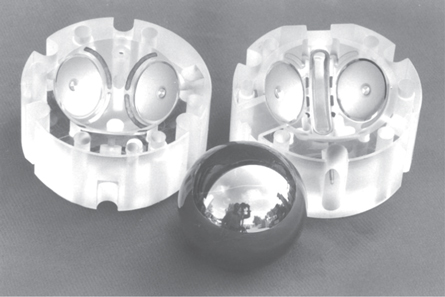
\includegraphics [scale=0.7] {sphere_suspension_photo}
  \caption{Сферический гироскоп с электростатическим подвесом. Фотография ротора и корпуса}
  \label{img:sphere_suspension_photo}
\end{figure}



Основным объектов исследования в работе является электростатический подвес сферического ротора  – основного структурного компонента отечественного электростатического гироскопа ЭСГ, спроектированного в Санкт-Петербургском ЦНИИ «Электроприбор» под руководством главного конструктора А.С. Анфиногенова. ЭСГ – сложнейший гироскопический прибор, работы по которому начались в СССР во второй половине 60-х годов, по сей день является наиболее точным датчиком первичной информации для инерциальных навигационных систем. 

Гироскоп ЭСГ состоит из стеклянной вакуумной камеры, на внутреннюю поверхность которой напылены шесть пар ортогонально расположенных электродов электрического подвеса. Внутри оболочки помещен полый тонкостенный сферической ротор, изготовленный из бериллия. Наружный диаметр ротора составляет 50 мм, вес ротора порядка 20 г, зазор между наружной поверхностью ротора и оболочкой 100 мкм, скорость вращения ротора достигает нескольких тысяч оборотов в минуту. Списывание углового положения ротора осуществляется фотооптическими датчиками \cite{History_ESG}.

К числу наиболее сложных задач, решаемых электростатическими гироскопами, относится навигационное обеспечение атомных подводных лодок, вооруженных баллистическими ракетами большого радиуса действия. Для обеспечения высокой точности ракет необходимо знать навигационные данные подводной лодки на момент старта с точностью на один-два порядка более высокой, чем та, которую обеспечивает навигационное счисление даже на коротких отрезках времени. 
Появление электростатических подвесов дало мощный толчок развитию гироскопической техники, неожиданно открылись совершенно новые интересные задачи \cite{Electropribor}.


%\newpage
%============================================================================================================================


%\newpage
%============================================================================================================================
           % Глава 1
\chapter{Анализ одномерной модели пассивного электростатического подвеса} \label{chapt2}

\section{Исследование одномерного пассивного электрического подвеса с постоянным напряжением, анализ его устойчивости. Теорема Ирншоу} \label{sect2_1}

Рассмотрим конфигурацию электростатического подвеса состоящего из проводящей незаряженной пластинки, помещенной между обкладками плоского конденсатора (рис.~\ref{img:simple_susp_1}). Окажется, что тело в такой системе не имеет устойчивых положений равновесия, электрические силы не зависят от положения тела, а результирующая электрических сил обращается в ноль. Действительно, запишем выражение для энергии электрического поля:
\begin{equation}
  \label{eq:simple_susp_energy_1}
  W_e = \frac{e^2}{2C_1}+\frac{e^2}{2C_2}
\end{equation}

\noindent где $e$ – заряд на конденсаторе, $C_1 = \frac{\epsilon_0 S}{h-y}$ – емкость между верхним электродом и пластиной, $C_2 = \frac{\epsilon_0 S}{h+y}$ – емкость между пластиной и нижним электродом, $h$ – половина расстояния между электродами, $y$ – смещение пластины вдоль вертикальной оси из среднего положения.

Таким образом, энергия $W_e$ (\ref{eq:simple_susp_energy_1}) не зависит от положения пластины, и результирующая сила, действующая на пластину со стороны электрического поля обращается в нуль.

\begin{figure}[ht]
    {\centering
        \hfill
        \subbottom[List-of-Figures entry][Двухэлектродный электростатический подвес\label{img:simple_susp_1}]{%
            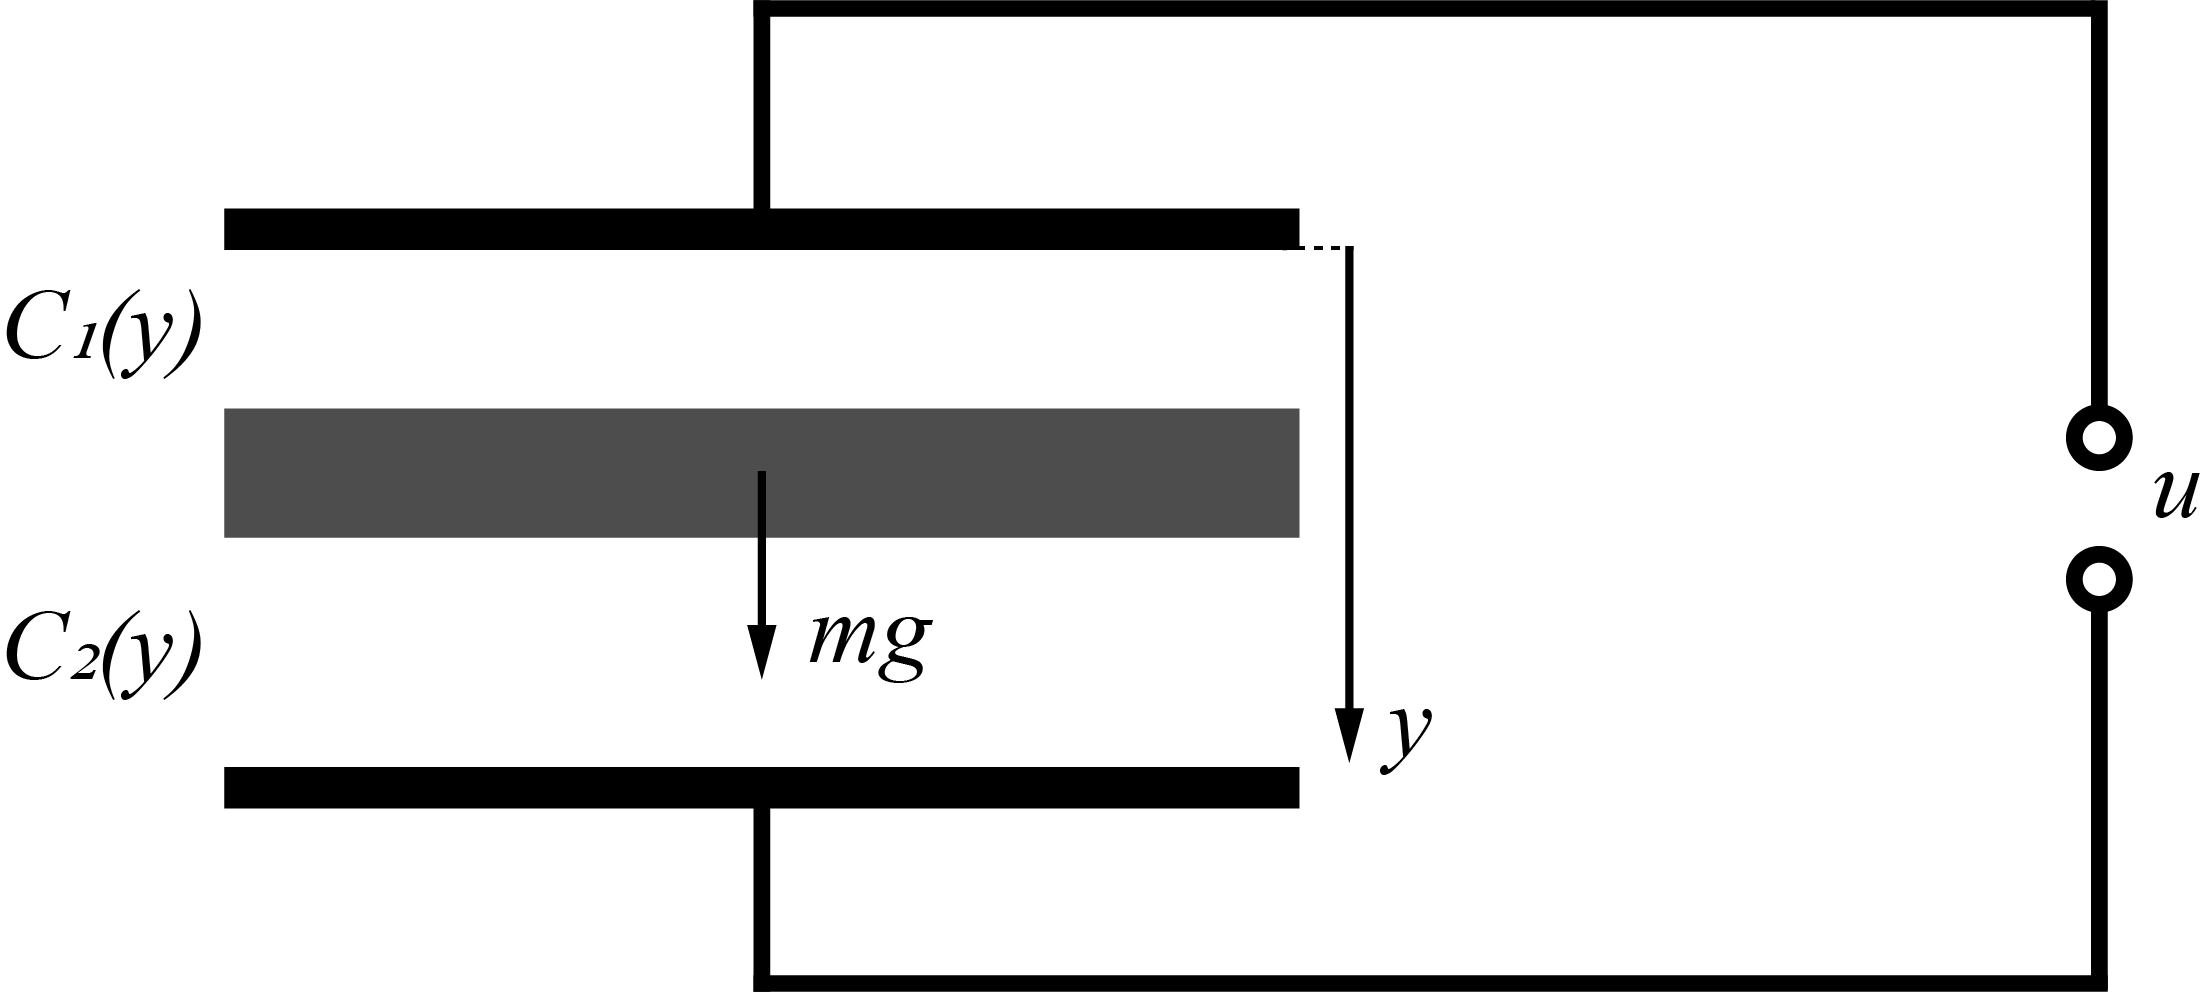
\includegraphics[width=0.49\linewidth]{simple_susp_1}}
        \hfill
        \subbottom[Четырехэлектродный электростатический подвес\label{img:simple_susp_2}]{%
            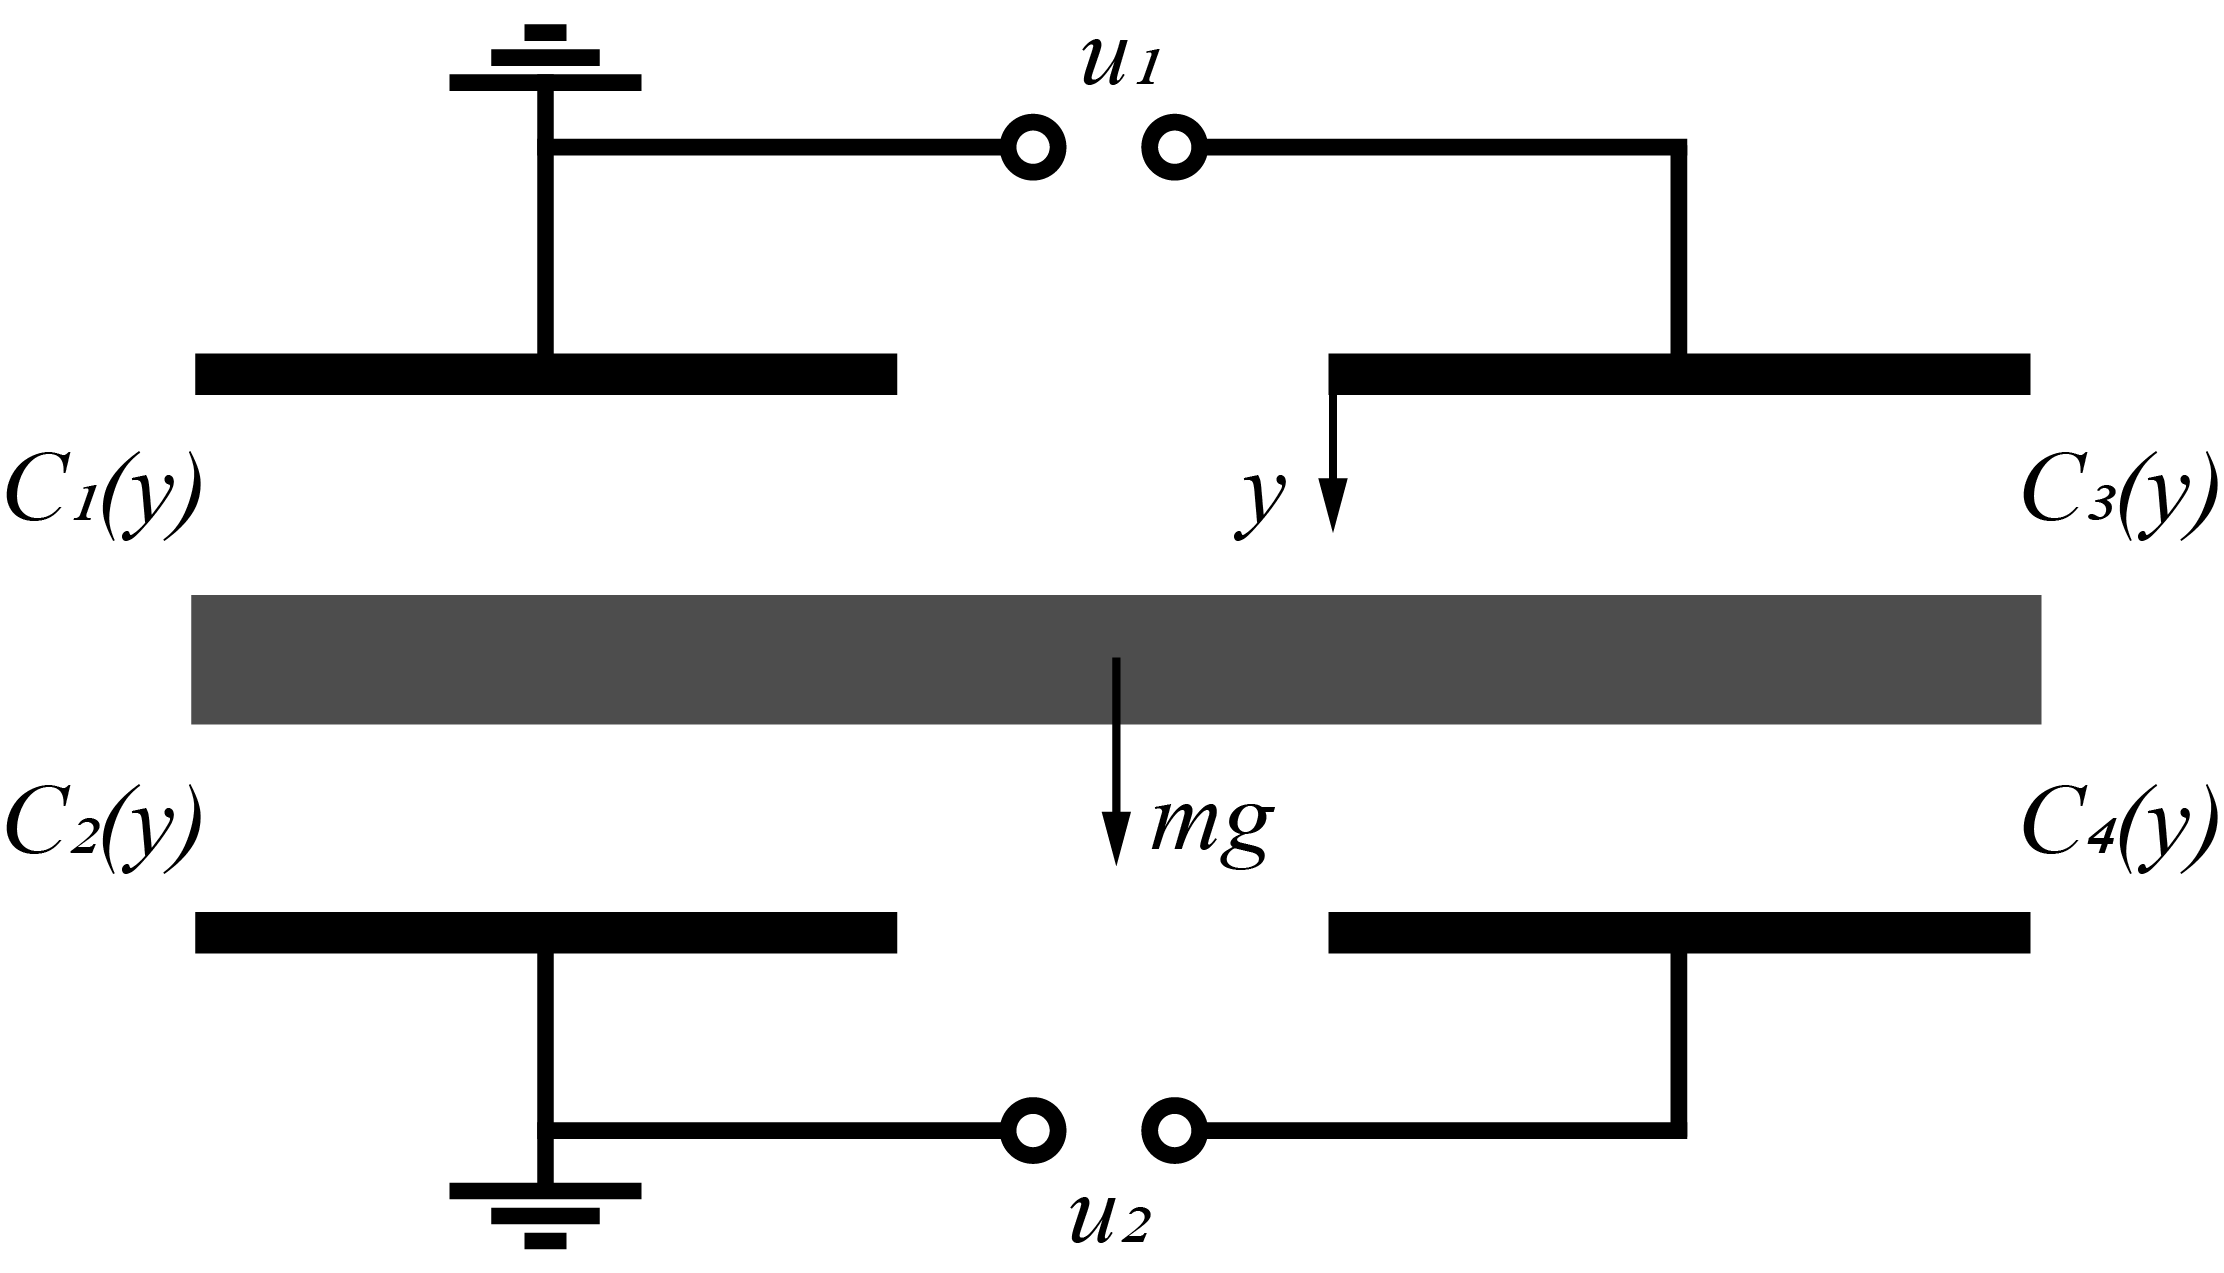
\includegraphics[width=0.49\linewidth]{simple_susp_2}}
        \hfill
    }
    \caption{Простейшие случаи электростатического подвеса}
    \label{img:simple_susp}
\end{figure}


Поэтому для создания одноосного электростатического подвеса незаряженного тела поместим его в электрическое поле созданное двумя парами электродов (рис. \ref{img:simple_susp_2}). Повторим процедуру и запишем уравнение энергии электрического поля для эквивалентной электрической схемы, изображенной на рис. \ref{img:simple_susp_equivalent}. Обозначим через $e_1$, $e_2$ заряды на конденсаторах $C_1$, $C_2$. Дифференцируя выражение энергии электрического поля, взятого с противоположным знаком, получим выражение для силы, действующей на твердое тело \cite{Martynenko}:

\begin{equation}
  \label{eq:simple_susp_energy_2}
  F(y) = \frac{\epsilon_0 S}{4} \left[\left( \frac{u_1}{h-y} \right)^2 - \left( \frac{u_2}{h+y} \right)^2\right],
\end{equation}

\noindent где $u_1$, $u_2$ – напряжения на электродах, связанные с зарядами на конденсаторах $e_1$ и $e_2$ соотношениями $u_1 = \frac{e_1}{C_1} + \frac{e_1+e_2}{C_3+C_4}$ и $u_2 = \frac{e_2}{C_2} + \frac{e_1+e_2}{C_3+C_4}$. 

\begin{figure}[ht] 
  \centering
  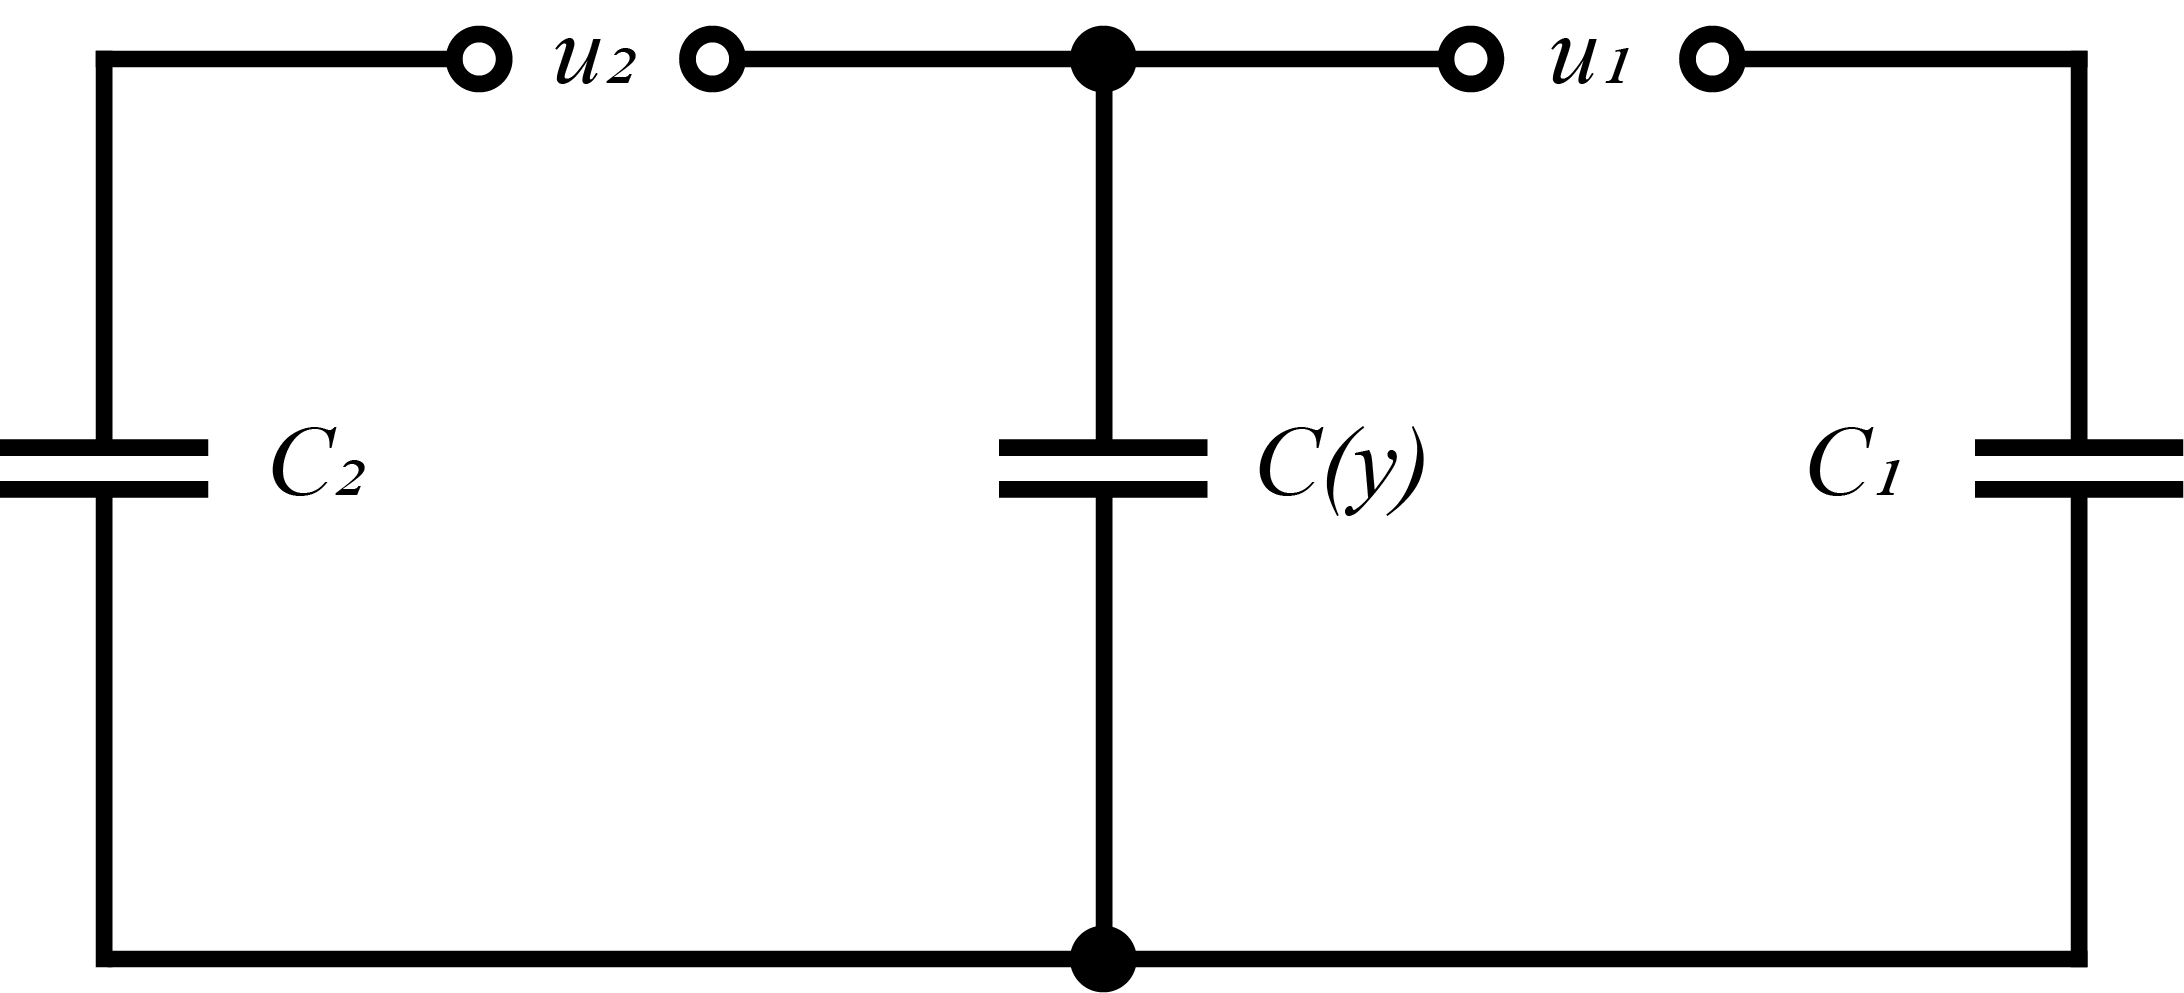
\includegraphics [scale=0.5] {simple_susp_equivalent}
  \caption{Эквивалентная электрическая схема четырехэлектродного электростатического подвеса}
  \label{img:simple_susp_equivalent}
\end{figure}

Функция $F(y)$ монотонно возрастает от $-\infty$ до $+\infty$ при $-h<y<h$. Положения равновесия тела в подвесе определяются из условия равенства веса тела $mg$ пондеромоторной силе $F$. На интервале $(-h, h)$ уравнение $F(y)=mg$ имеет единственное решение, потенциальная энергия при этом будет иметь максимум, а положение равновесия будет неустойчивым.

Данная ситуация является следствием теоремы Ирншоу о неустойчивости электрических систем \cite[с.~92]{Tamm}, которая говорит о том, что нахождение проводящего тела в состоянии устойчивого равновесия в электрическом поле под действием только электрических сил невозможно.


%\newpage
%============================================================================================================================

\section{Обоснованность применения теории электростатики} \label{sect1_1_1}

Твердое тело в электростатическом подвесе находится в вакуумированной полости, ограниченной конечным числом проводящих электродов. Строго говоря, электрическое поле, потенциалы на электродах которого являются функциями от фазовых координат и времени, не является электростатическим. Тем не менее, можно показать, что выполняются условия квазистационарности, которые сводятся к требованию \cite{Tamm}:
\[
T^* \gg \tau,
\]
где $T^*$ – характерное время в движении твердого тела, $\tau = L^*/c$ – время запаздывания, $L^*$ – характерный размер системы, $c$ – скорость света. При $T^* \sim 10^{-3}$ с, $L^* \sim 10^{-3}$ см время $\tau \sim 0.3 \cdot 10^{-9}$ с, $\tau/T^* \sim 10^{-6}$.
Поэтому, пренебрегая запаздыванием системы, можем с приемлемой для практики точностью считать поле стационарным и в каждый момент времени решать задачу электростатики \cite{Martynenko}.

\section{Исследование одномерного пассивного электростатического подвеса с переменным напряжением} \label{sect2_2}

\subsection{Методы стабилизации тела в электростатическом подвесе. Простейшие системы управления, доставляющие асимптотическую устойчивость положению равновесия} \label{subsect2_2_1}

\begin{figure}[ht] 
  \centering
  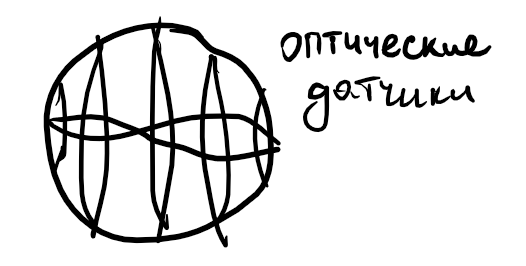
\includegraphics [scale=1.0] {optical_sensors}
  \caption{Рисунок на роторе сферического гироскопа для фиксации положения оптическим датчиком}
  \label{img:optical_sensors}
\end{figure}

Для создания устойчивого положения равновесия твердого тела в электростатическом подвесе необходимо управление потенциалами электродов. Обычно положение твердого тела в электростатическом подвесе измеряется специальными датчикам (емкостными или оптическими, рис. \ref{img:optical_sensors}) \cite{Electropribor}. Электростатические подвесы с системами слежения, то есть такие, напряжения на электродах которых изменяются в зависимости от положения тела, называют активными. Простейшую функцию пондеромоторных сил в активной системе можно представить в виде нелинейного закона управления:
\begin{equation}
  \label{eq:simple_susp_active_force}
  F(y) = \left\{
    \begin{alignedat}{2}
        &F_1(y), \quad &\text{eсли }& -h\geqslant y \geqslant -\frac{V}{k}, \\
        &F_2(y), \quad &\text{eсли }& -\frac{V}{k}\geqslant y \geqslant \frac{V}{k}, \\
        &F_3(y), \quad &\text{eсли }& \frac{V}{k}\geqslant y \geqslant -h,
    \end{alignedat}
    \right.
\end{equation}

\noindent где $V$ – некоторое постоянное «опорное» напряжение, $k$ – коэффициент усиления следящей системы, причем предполагается, что $k>V/h$. При $k>V/h$ график функции $F(y)$ построен на рис. \ref{img:active_susp_force_plot}.
Напряжения на электродах в таких системах могут быть не только функциями координаты смещения твердого тела, но и зависеть от его скорости, что позволяет исключить негативное влияние наличия запаздывания в следящей системе. Так как в действительности в соотношения $F(y)$ войдет значение координаты $y$, зависящей от некоторого предыдущего момента времени, что приведет к нарастанию амплитуды колебаний тела. 

\begin{figure}[ht] 
  \centering
  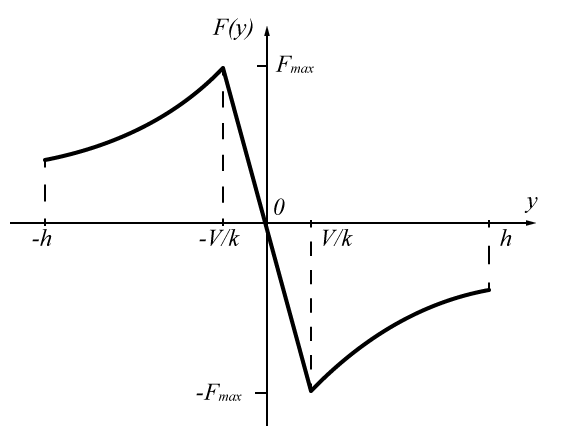
\includegraphics [scale=0.5] {active_susp_force_plot}
  \caption{Зависимость силы $F$ от смещения $y$ в активном электростатическом подвесе}
  \label{img:active_susp_force_plot}
\end{figure}

\subsection{Аналитическое исследование одноосного пассивного электростатического подвеса} \label{subsect2_2_2}

Справится с естественной неустойчивостью электростатических подвесов без использования активных следящих систем позволяют, например, пассивные или резонансные подвесы. Простейшая схема одноосного пассивного электростатического подвеса представлена на рисунке \ref{img:pas_susp_scheme}. Верхняя пластина плоского конденсатора является неподвижной, а нижняя пластина должна удерживаться на некотором расстоянии от верхней пластины в положении, когда вес пластины уравновешивается силой притяжения, действующей на проводник в электрическом поле, созданном между обкладками конденсатора.

Электрическая цепь рассматриваемой электромеханической системы образована индуктивностью $L$, конденсатором $C$, омическим сопротивлением $R$. ЭДС внешнего источника, подключенного к цепи, изменяется по синусоидальному закону $u = u_0 \sin \omega t$, $u_0$ – амплитуда, $\omega$ – частота.

\begin{figure}[ht] 
  \centering
  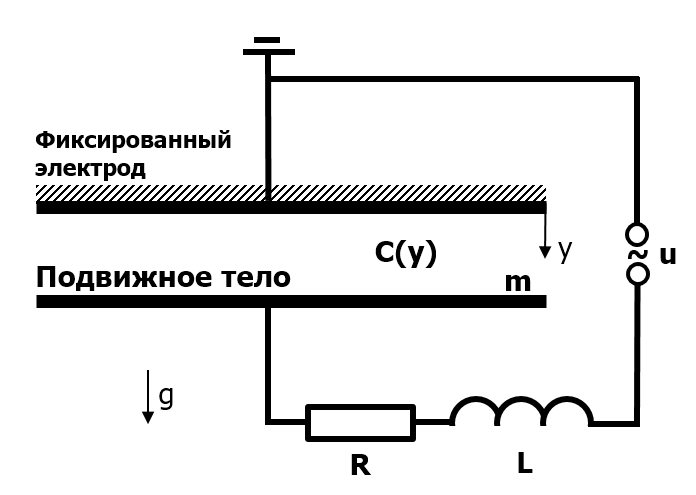
\includegraphics [scale=0.5] {pas_susp_scheme}
  \caption{Схема одноосного пассивного электростатического подвеса}
  \label{img:pas_susp_scheme}
\end{figure}

Запишем уравнения движения данной схемы, для этого обозначим через $m$ массу подвижной пластины и введем вертикальную ось $y$. Выберем начало отсчета в точке $O$, принадлежащей верхнему фиксированному электроду, тогда в реальной системе координата нижней пластины $y<0$.
В качестве обобщенных координат выберем координату $y$ подвижной пластины и заряд на конденсаторе $C(y) = \epsilon_0 S/y$. Кинетическая энергия пластины $T = m \dot y^2/2$, потенциальная энергия силы тяжести $\Pi = mgy$. Магнитная энергия электрической цепи $W_m=L \dot e^2/2$, где $\dot e \equiv i$ – ток в цепи. Энергия электрического поля, локализованного между обкладками конденсатора, без учета краевых эффектов
\[
W_e = \frac{e^2}{2C(y)} = - \frac{e^2 y}{2 \epsilon_0 S}.
\]

Функция Лагранжа для рассматриваемой электромеханической системы принимает вид
\[
L = T - \Pi + W_m - W_e = \frac{1}{2}m \dot y^2 - mgy + \frac{1}{2}L_1 \dot e^2 + \frac{e^2 y}{2 \epsilon_0 S}.
\]

Пластина подвешена в вакууме, силой трения при движении пластины пренебрегаем. Тогда диссипативная функция Рэлея будет определятся только потерями в электрической цепи $\Psi = \frac{1}{2}R \dot e^2$. Учитывая, что обобщенные неконсервативные силы механической природы отсутствуют, запишем уравнения Лагранжа–Максвелла \cite{Martynenko_andyn}
\[
\frac{d}{dt} \left( \frac{\partial L}{\partial \dot e} \right) - \frac{\partial L}{\partial e} + \frac{\partial \Psi}{\partial \dot e} = u, \quad
\frac{d}{dt} \left( \frac{\partial L}{\partial \dot y} \right) - \frac{\partial L}{\partial y} + \frac{\partial \Psi}{\partial \dot y} = 0.
\]

Выполняя операции дифференцирования, получаем уравнения движения
\begin{equation}
  \label{eq:pas_susp_motion}
    \begin{alignedat}{2}
    &L \ddot e + R \dot e - \frac{e y}{\epsilon_0 S} = u_0 \sin \omega t, \\
    &m \ddot y + m g - \frac{e^2}{2 \epsilon_0 S} = 0.
    \end{alignedat}
\end{equation}

Система уравнений (\ref{eq:pas_susp_motion}) представляет систему нелинейных неавтономных дифференциальных уравнений 4-го порядка относительно переменных $y, e$, нахождение аналитического решения этой системы не представляется возможным.
Построим приближенное решение системы (\ref{eq:pas_susp_motion}), приняв $y$ в первом уравнении за постоянный параметр. Такое предположение возможно в силу того, что в реальных системах частота задающего напряжение $\omega$  велика по сравнению с механическими колебаниями $y$. В таком случае, первое уравнение системы (\ref{eq:pas_susp_motion}) принимает вид линейного дифференциального уравнения с постоянными коэффициентами. Решение данного уравнения представляет собой сумму общего и частного решений \cite{Martynenko}
\begin{equation}
  \label{eq:pas_susp_charge}
    e = \frac{u_0 \sin (\omega t + \phi)}{\sqrt{\left(L \omega^2 + \frac{y}{\epsilon_0 S} \right)^2 
    + \left( R \omega \right)^2}} + e_{\text{общ}},
\end{equation}

\noindent где $\phi$ – сдвиг по фазе между вынужденным колебанием и внешней силой, $e_{\text{общ}}$ – общее решение однородного уравнения, т.е. решение первого уравнения (\ref{eq:pas_susp_motion}) при $u_0=0$. Вне малого начального интервала времени общее решение $e_{\text{общ}}$ в силу того, что оно является экспоненциально убывающей функцией времени, можно считать равным нулю. Подставим (\ref{eq:pas_susp_charge}) во второе уравнение (\ref{eq:pas_susp_motion}) и заменим функцию $\sin{\omega t + \phi}^2$ его средним значением, тогда получим нелинейное дифференциальное уравнение второго порядка относительно переменной $y$
\begin{equation}
  \label{eq:pas_susp_sol_1}
    m \ddot y +mg -f(y)=0, \quad f(y) = \frac{1}{2 \epsilon_0 S} \frac{u_0^2}{\left(L \omega^2 + \frac{1}{\epsilon_0 S} y \right)^2 
    + \left( R \omega \right)^2}.
\end{equation}

Построим график функции $f(y)$ (рис. \ref{img:pas_susp_force_theory}). Функция $f(y)$ на интервале $-\infty < y < -L \epsilon_0 S \omega^2 $ возрастает от нуля до некоторого положительного значения, а затем при $-L \epsilon_0 S \omega^2 < y < 0 $ функция монотонно убывает. Для определения положений равновесия  положим $\ddot y =0$, тогда $mg = f(y)$ – уравнение для определения равновесных положений твердого тела в электростатическом подвесе.

\begin{figure}[ht] 
  \centering
  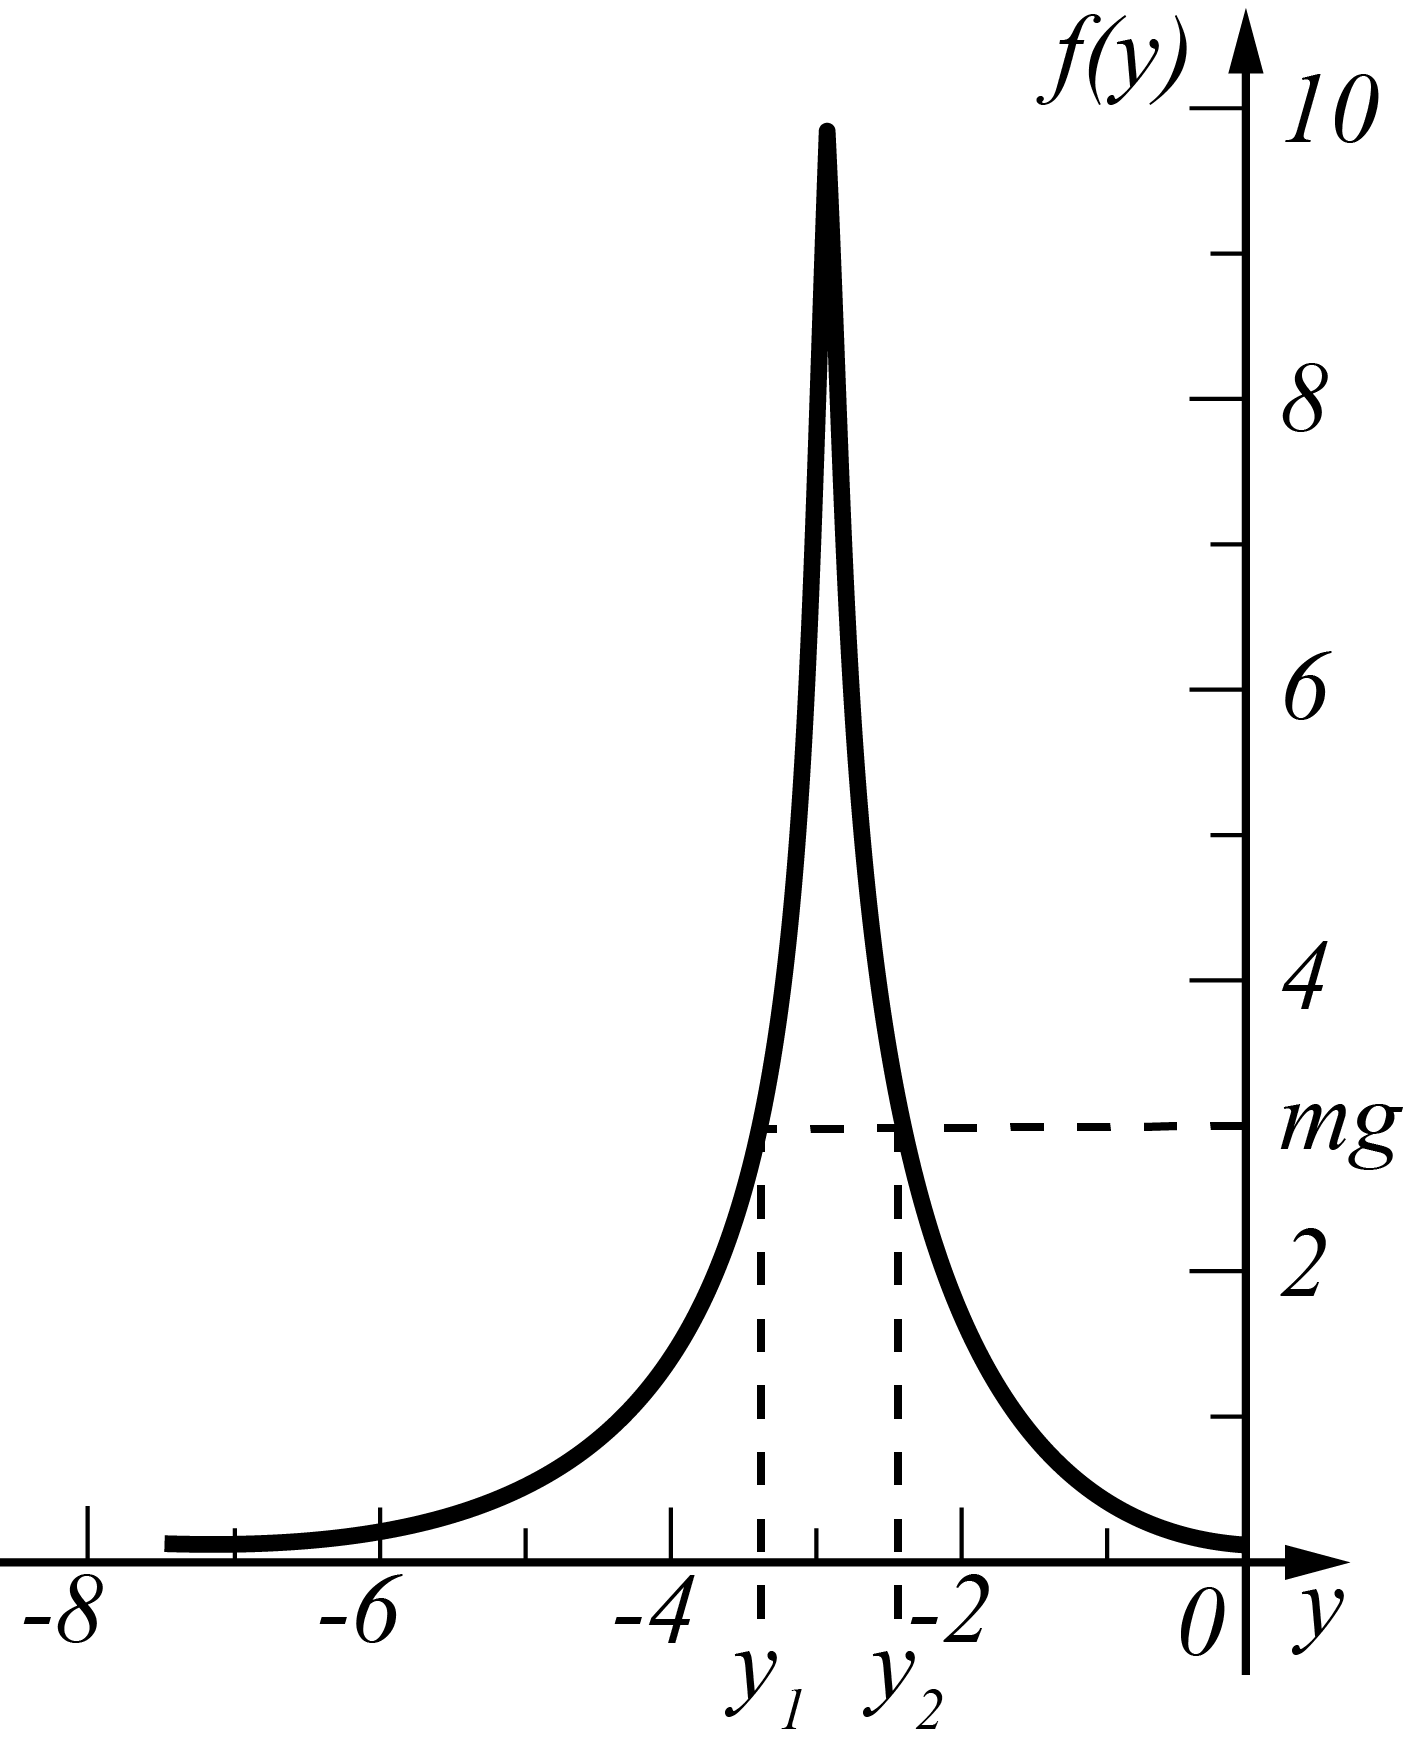
\includegraphics [scale=0.5] {pas_susp_force_theory}
  \caption{График функции $f(y)$}
  \label{img:pas_susp_force_theory}
\end{figure}

Максимальное значение функции $f_{max} = \frac{u_0^2}{4 \epsilon_0 S (R \omega)^2}$ отвечает за максимальный вес твердого тела, который способен удержать электростатический подвес. Будем считать, что $mg<f_{max}$. Тогда прямая $mg$ на рис. \ref{img:pas_susp_force_theory} пересекает $f(y)$ в двух точках $y=y_1, y=y_2$. В этом случае электростатический подвес имеет два положения равновесия.

Потенциальная энергия имеет вид (\ref{eq:pas_susp_potential}), ее график представлен на рис.  \ref{img:pas_susp_potential}. По теореме Лагранжа–Дирихле устойчивым оказывается положение равновесия $y = y_2$, положение равновесия $y=y_1$ неустойчиво.

\begin{equation}
  \label{eq:pas_susp_potential}
    \ddot y + \frac{\partial \Pi}{\partial y} = 0, \quad 
    \Pi(y) = gy - \frac{u_0^2}{4R m \omega} \arctan{ \frac{L \omega^2 + \frac{y}{\epsilon_0 S}}{R\omega} }
\end{equation}

\begin{figure}[ht] 
  \centering
  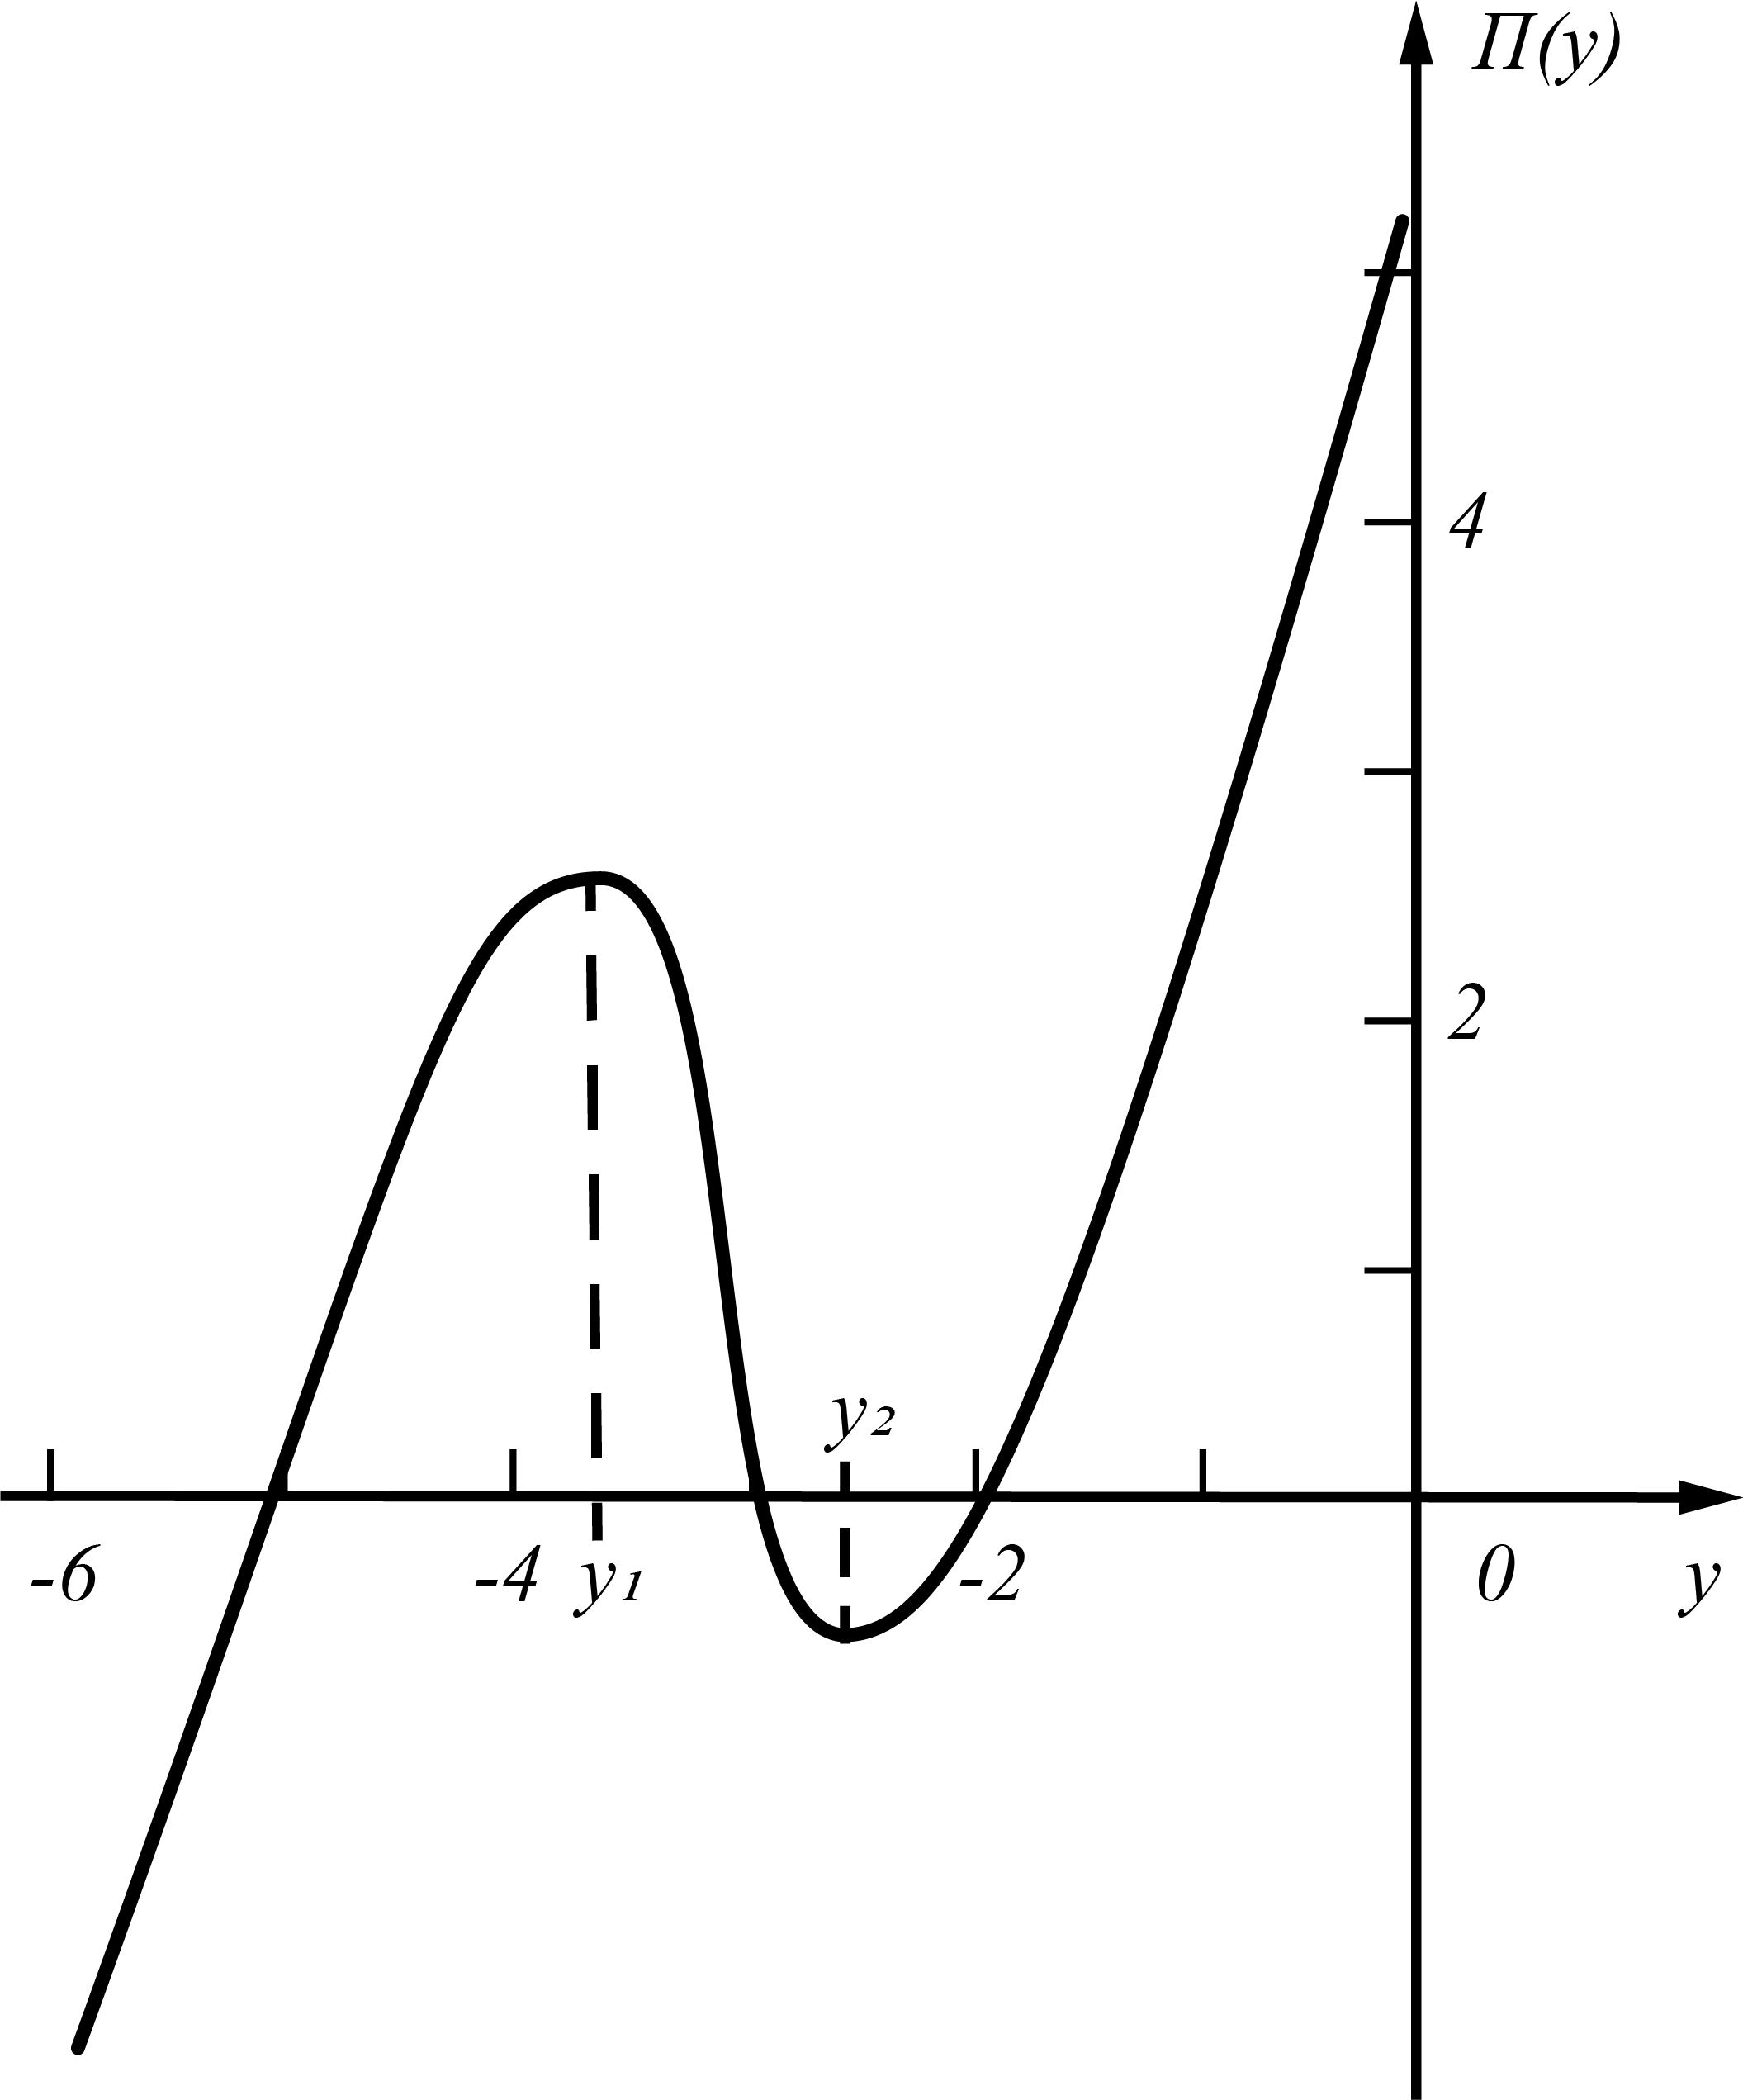
\includegraphics [scale=1] {pas_susp_potential}
  \caption{График функции $\Pi(y)$}
  \label{img:pas_susp_potential}
\end{figure}

Физический смысл работы пассивного подвеса заключается в том, что при удалении тела от фиксированного электрода пондеромоторная электрическая сила возрастает, возвращая тело в положение $y = y_2$. И наоборот, при приближении тела к электроду пондеромоторная электрическая сила уменьшается, становясь меньше, чем сила тяжести, и тело возвращается обратно в положение равновесия.


\subsection{Обзор возможностей программной системы ANSYS для решения задач электромеханики. Методы определения пондеромоторных усилий в подвесах с применением численных решений ANSYS} \label{subsect2_3_2}

Программная система конечно-элементного анализа ANSYS предоставляет возможность моделирования электромеханических задач несколькими способами \cite{Ansys_coupled_field}:
\begin{enumerate}
  \item Прямое решение связанной задачи (Direct coupled-field analysis)
  \item Использование электромеханических элементов-преобразователей \textit{TRANS126} (Transducer elements)
  \item Параллельное решение двух связанных задач (Multi-field analysis)
  \item Прямое разложение по собственным формам (Reduced order modelling)
\end{enumerate}


\textbf{Прямое решение связной задачи} (Direct coupled-field analysis) реализуется благодаря совмещению в одном конечном элементе как трансляционных, так и электрических степеней свободы. Метод позволяет решать задачу в один шаг по времени, не разделяя электрическую и механическую задачи, более того, сочетание трансляционной и электрической степеней свободы позволяет учитывать неоднородности моделируемого электрического поля за счет геометрии конечных элементов.

Недостатками данного способа решения являются необходимость в случае сложной геометрии межэлектродного пространства использовать большое количество конечных элементов, несимметричность общей матрицы, приводящая к увеличению времени счета.

Метод предполагает использование специальных конечных элементов, например, двумерных квадратичных 8-ми узловых элементов \textit{PLANE223} или трехмерных квадратичных 12-ти узловых \textit{SOLID226}. Каждый узел элемента данных типов может содержать до 5 степеней свободы. Для решения связанной электромеханической задачи выберем электроупругую опцию элемента \textit{KEYOPT(1)=1001}, тогда каждый узел будет иметь 3 трансляционных и одну электрическую степени свободы: UX, UY, UZ, VOLT.


\textbf{Элементы преобразователи \textit{TRANS126}} представляют собой одномерные двух-узловые элементы с двумя степенями свободы в каждом узле: трансляционной (на выбор: UX, UY или UZ) и электрической (VOLT), Элементы данного типа предназначены для преобразования электрической энергии в механическую и наоборот, таким образом, позволяют связать электрические и механические степени свободы. 

Принцип работы заключается в наличии в элементе зависимости электрической емкости $C$ от зазора $\delta$ между его узлами
\[
C = C(\delta), \quad \delta = \delta_0 +u_1 - u_2,
\]
\noindent где $\delta_0$ – начальный зазор, $u_1, u_2$ – координаты $1$-го и $2$-го узлов элемента соответственно.

Существует возможность задания зависимости $C(\delta)$ как в форме полинома 4-ой степени, так и парами чисел «емкость–зазор». Расчет зависимости $C(\delta)$ производится предварительно отдельным расчетом, например, с помощью макроса \textit{CMATRIX} \cite[с.~275]{Ansys_command_reference}. Таким образом, в элементах–преобразователях рассчитывается зависимость электрической силы от положения тела. Появляется возможность схематизировать сложное электрическое поле совокупностью конечного числа элементов–преобразователей (рис. \ref{img:multi_trans126}).

\begin{figure}[ht] 
  \centering
  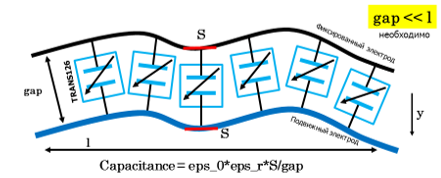
\includegraphics [scale=1] {multi_trans126}
  \caption{Пример схематизации электрического поля множеством элементов–преобразователей \textit{TRANS126}}
  \label{img:multi_trans126}
\end{figure}


Преимуществами данного метода являются простота построения конечно-элементной модели, малое расчетное время, а также возможность учета механического контакта пластин конденсатора. Вынужденная схематизация электрического поля является одним из недостатков метода, не позволяющая учитывать неоднородности электрического поля.



В данной работе не уделено внимание подробному рассмотрению методов \textbf{параллельного решения связанных задач} (Multi-Field analysis) и \textbf{прямого разложения по собственным формам} (Reduced order modelling). Отметим лишь, что принцип работы первого строится на итерационном решении механической и электрической задач, значения усилий и перемещений в данном методе интерполируются между несвязанными моделями. Основным недостатком такого подхода является необходимость перестраивания сетки на каждом итерационном шаге, что негативно отражается на времени счета. Метод прямого разложения, как следует из названия, основывается на разложении электромеханической задачи по собственным формам. Отличительной чертой метода является его эффективность при решении динамических задач на больших промежутках времени. Оба метода подробно описаны в \cite{Ansys_coupled_field}.


\subsection{Конечно-элементное моделирование и анализ одномерного пассивного электростатического подвеса с переменным напряжением} \label{subsect2_2_3}

Аналитическое исследование одноосного пассивного электростатического подвеса проведено ранее в разделе \ref{subsect2_2_1}. Для получения численных оценок поведения подвеса обратимся к возможностям конечно-элементной программной системы ANSYS Mechanical, которые были разобраны в предыдущем разделе \ref{subsect2_2_2}.

\begin{figure}[ht] 
  \centering
  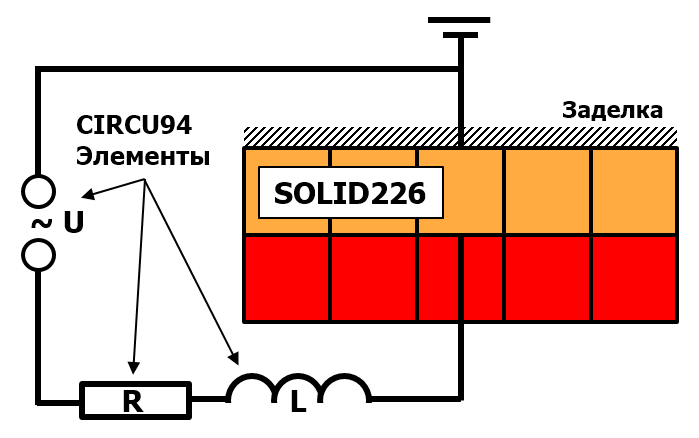
\includegraphics [scale=0.5] {pas_susp_solid226_scheme}
  \caption{Расчетная схема конечно-элементной постановки методом прямого решения связанной задачи}
  \label{img:pas_susp_solid226_scheme}
\end{figure}

Построим расчетную конечно-элементную модель для прямого решения связанной задачи. Элементами \textit{SOLID226} моделируем пространство между электродом и твердым телом электростатического пассивного подвеса (рис. \ref{img:pas_susp_scheme}). На узлы, принадлежащие верхнему электроду, задаем связь равенства между собой электрических VOLT и трансляционных UX, UY, UZ степеней свободы (\textit{Coupling}–связь), ту же связь задаем и на узлы соответствующие твердому телу. Помимо этого, на узлы, принадлежащие поверхности твердого тела, применяем граничное условие первого рода VOLT $=0$. Массу твердого тела моделируем $MASS21$ элементом. Разность потенциалов на противоположных гранях получившегося объема, т.е. разность потенциалов между электродом и телом, порождают в узлах силы, эквивалентные пондеромоторным электрическим силам, связывая тем самым механическую и электрическую задачи. Электрическую цепь моделируем одномерными элементами \textit{CIRCU94}, содержащими одну электрическую степень свободы VOLT. Схема расчетной модели для метода прямого решения связанной задачи с использованием \textit{SOLID226} элементов представлена на рис. \ref{img:pas_susp_solid226_scheme}.

Выбор параметров системы проводим на основе аналитических оценок раздела \ref{subsect2_2_1}. Для моделирования одноосного пассивного подвеса методом конечных элементов с использованием метода прямого решения связанной задачи приняты следующие параметры:

\begin{itemize}
  \item Амплитуда источника напряжения $u_0 = 10\ \text{В}$
  \item Частота источника напряжения $\omega = 40\ \text{кГЦ}$
  \item Сопротивление резистора $R = 300\ \text{Ом}$
  \item Индуктивность $L = 2\ \text{мГн}$
  \item Номинальный зазор $\delta_0 = 3\ \text{мкм}$
  \item Масса удерживаемого твердого тела $m = 6.25\ \text{г}$
  \item Площадь фиксированного электрода $S = 50\ \text{см}^2$
\end{itemize}

В силу большого времени счета ограничимся решением динамической задачи данным методом с фиксированным твердым телом, т.~е. при $y = const = \delta_0$. 

Решение производим путем динамического конечно-элементного анализа \textit{(ANTYPE,TRANS)} методом Ньютона-Рафсона (модифицированный метод касательных) \cite{Ansys_theory_reference}, шаг интегрирования задаем вручную, для этого проанализируем сходимость численного конечно-элементного решения, построив график зависимости значения напряжения на верхнем электроде от величины шага интегрирования (рис. \ref{img:pas_susp_solid226_conv}). 


\begin{figure}[ht] 
  \centering
  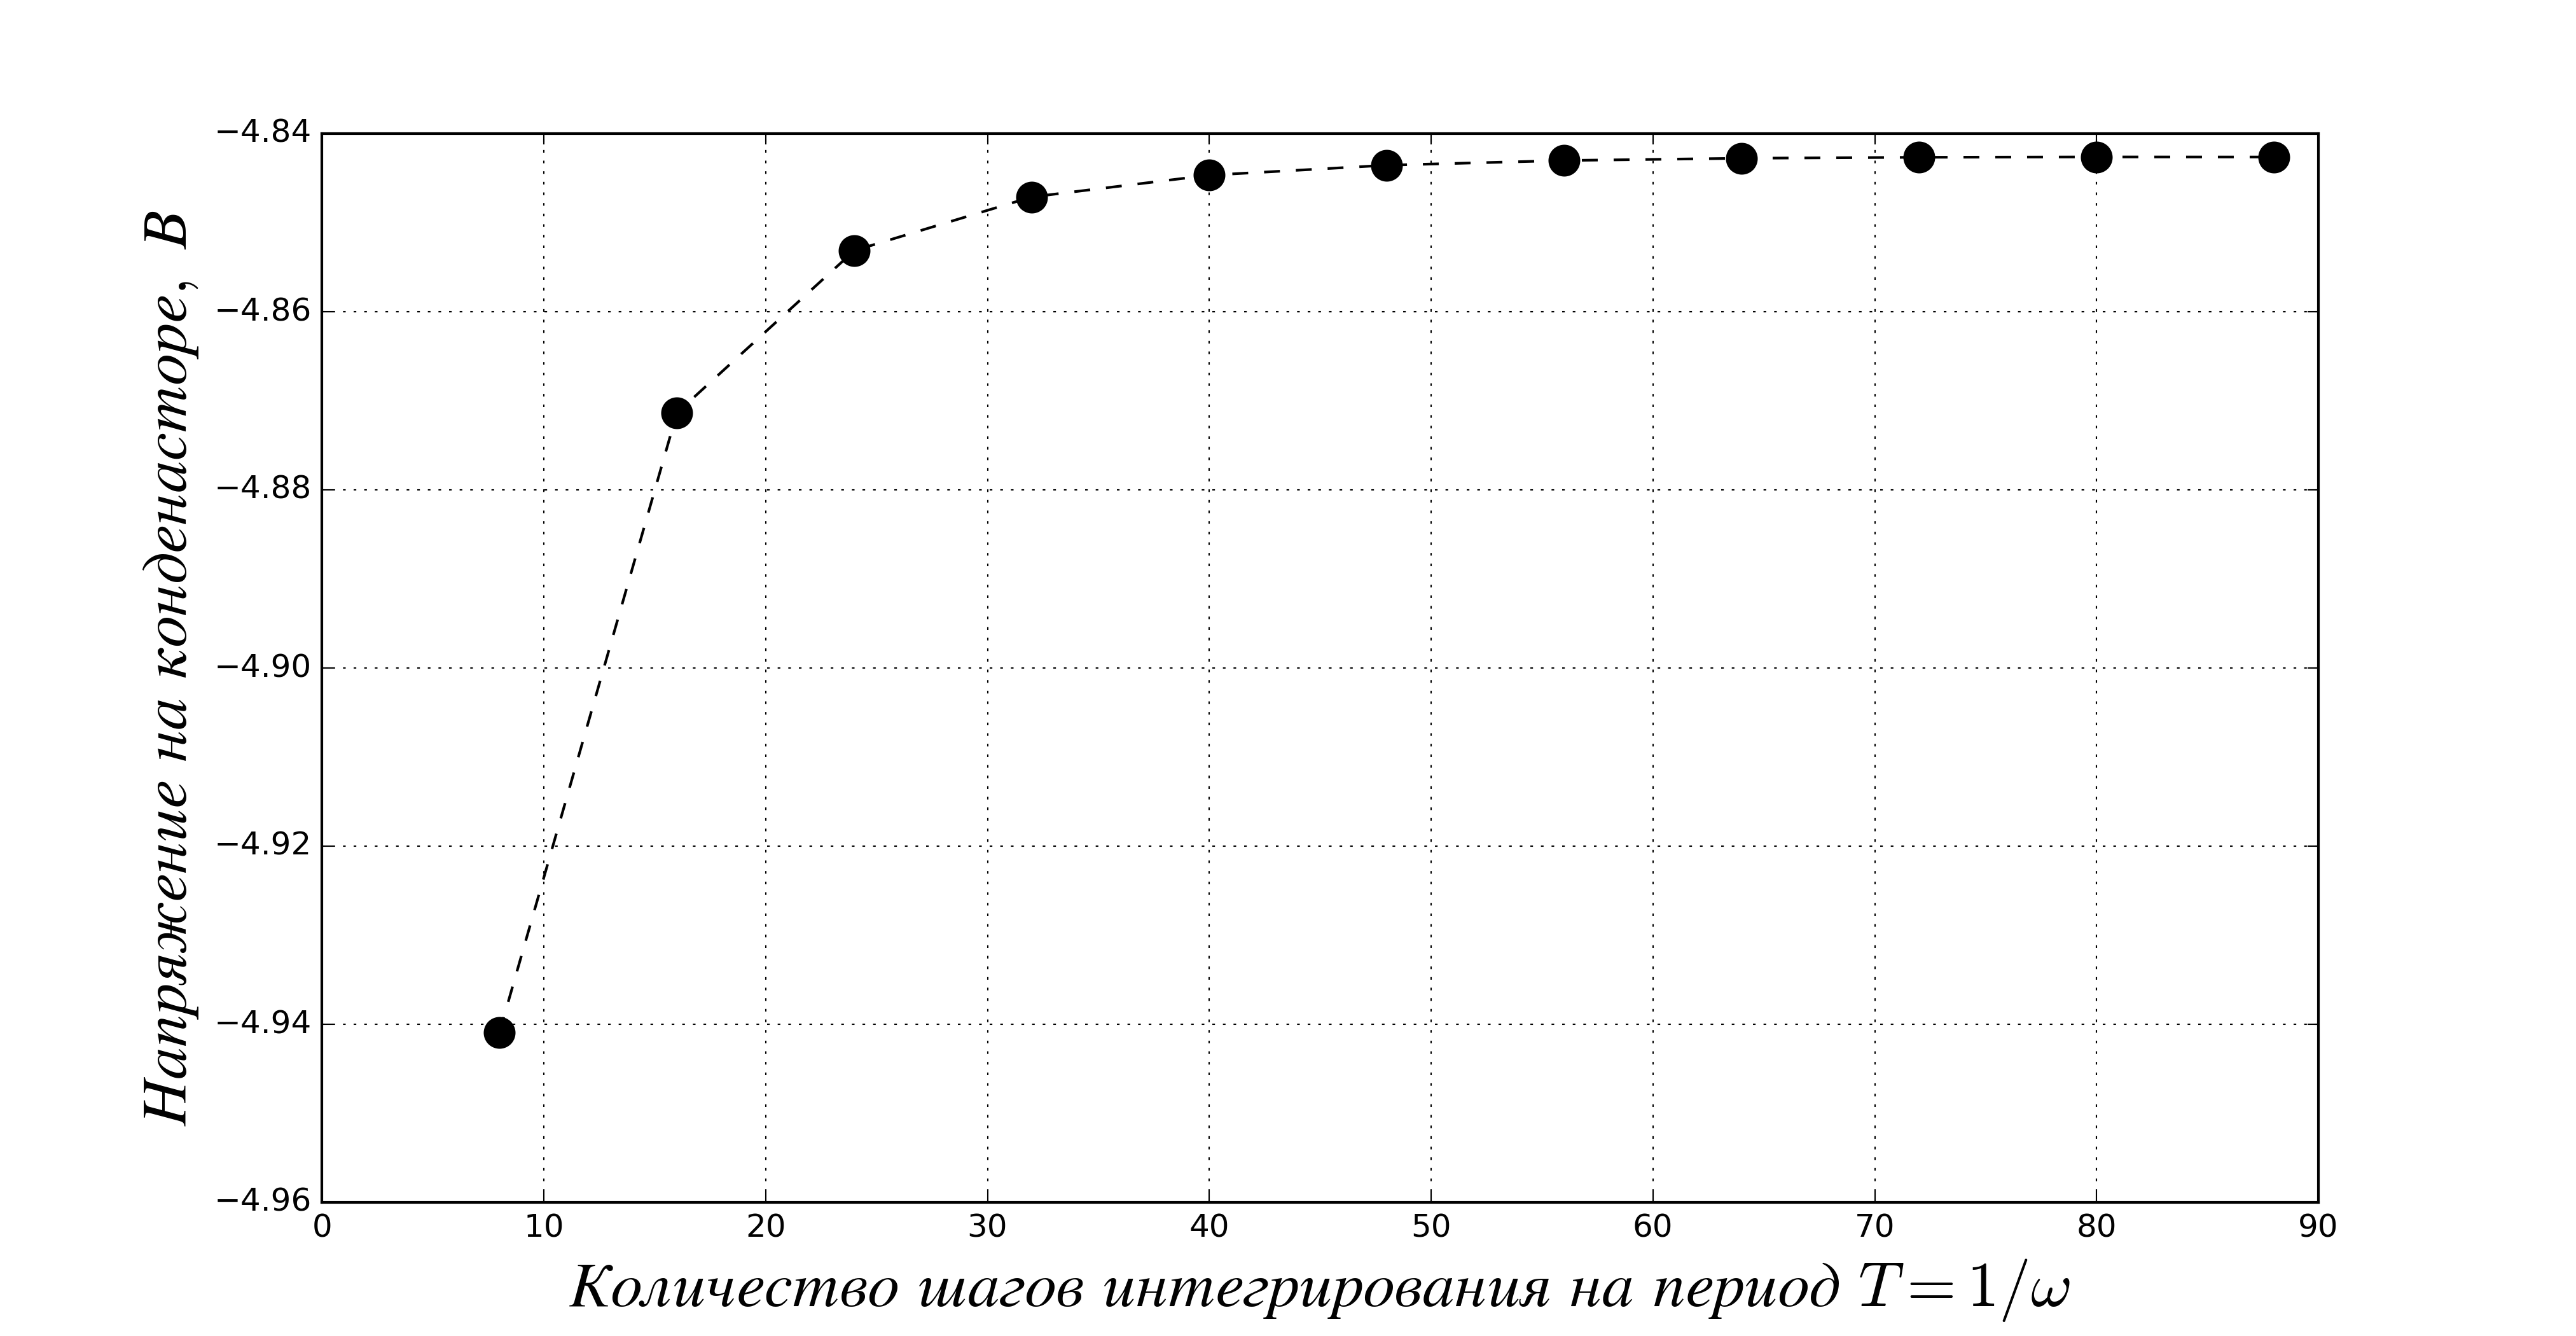
\includegraphics [scale=0.5] {pas_susp_solid226_conv}
  \caption{График сходимости метода прямого решения $y(N)$, где $N$ – количество шагов интегрирования на один период $T=1/\omega$.}
  \label{img:pas_susp_solid226_conv}
\end{figure}

Зададимся точностью $\epsilon = 0.0001$, т.~е. будем считать решение сошедшимся, если угловой коэффициент касательной к графику \ref{img:pas_susp_solid226_conv} не превышает $\epsilon$. Таким образом, минимальное количество шагов интегрирования на один период источника ЭДС необходимое для получения удовлетворяющего принимаем равным $64$, т.~е. $dt_{max}=\frac{1}{64} \cdot T$, где $T = \frac{1}{\omega}$ – период, ${\omega}$ – частота источника напряжения.

Результатом расчета имеем зависимости от времени напряжения на электроде $U$ и электрической силы $F_e$, представленные на рис. \ref{img:pas_susp_solid226_sol}. Отклонение решения методом конечных элементов в модели с 50-ю элементами от прямого численного интегрирования уравнений (\ref{eq:pas_susp_motion}) не превышает $14\%$, а с 500 элементами – $2.3\%$, т.~е. при увеличении плотности разбиения демонстрируется тенденция приближения конечно-элементного решения к некоторому решению, близкому к численно интегрированному уравнению (\ref{eq:pas_susp_motion}). Более подробный анализ сходимости решения от количества разбиений в работе не приведен по причине высокой ресурсоемкости метода.

\begin{figure}[ht] 
  \centering
  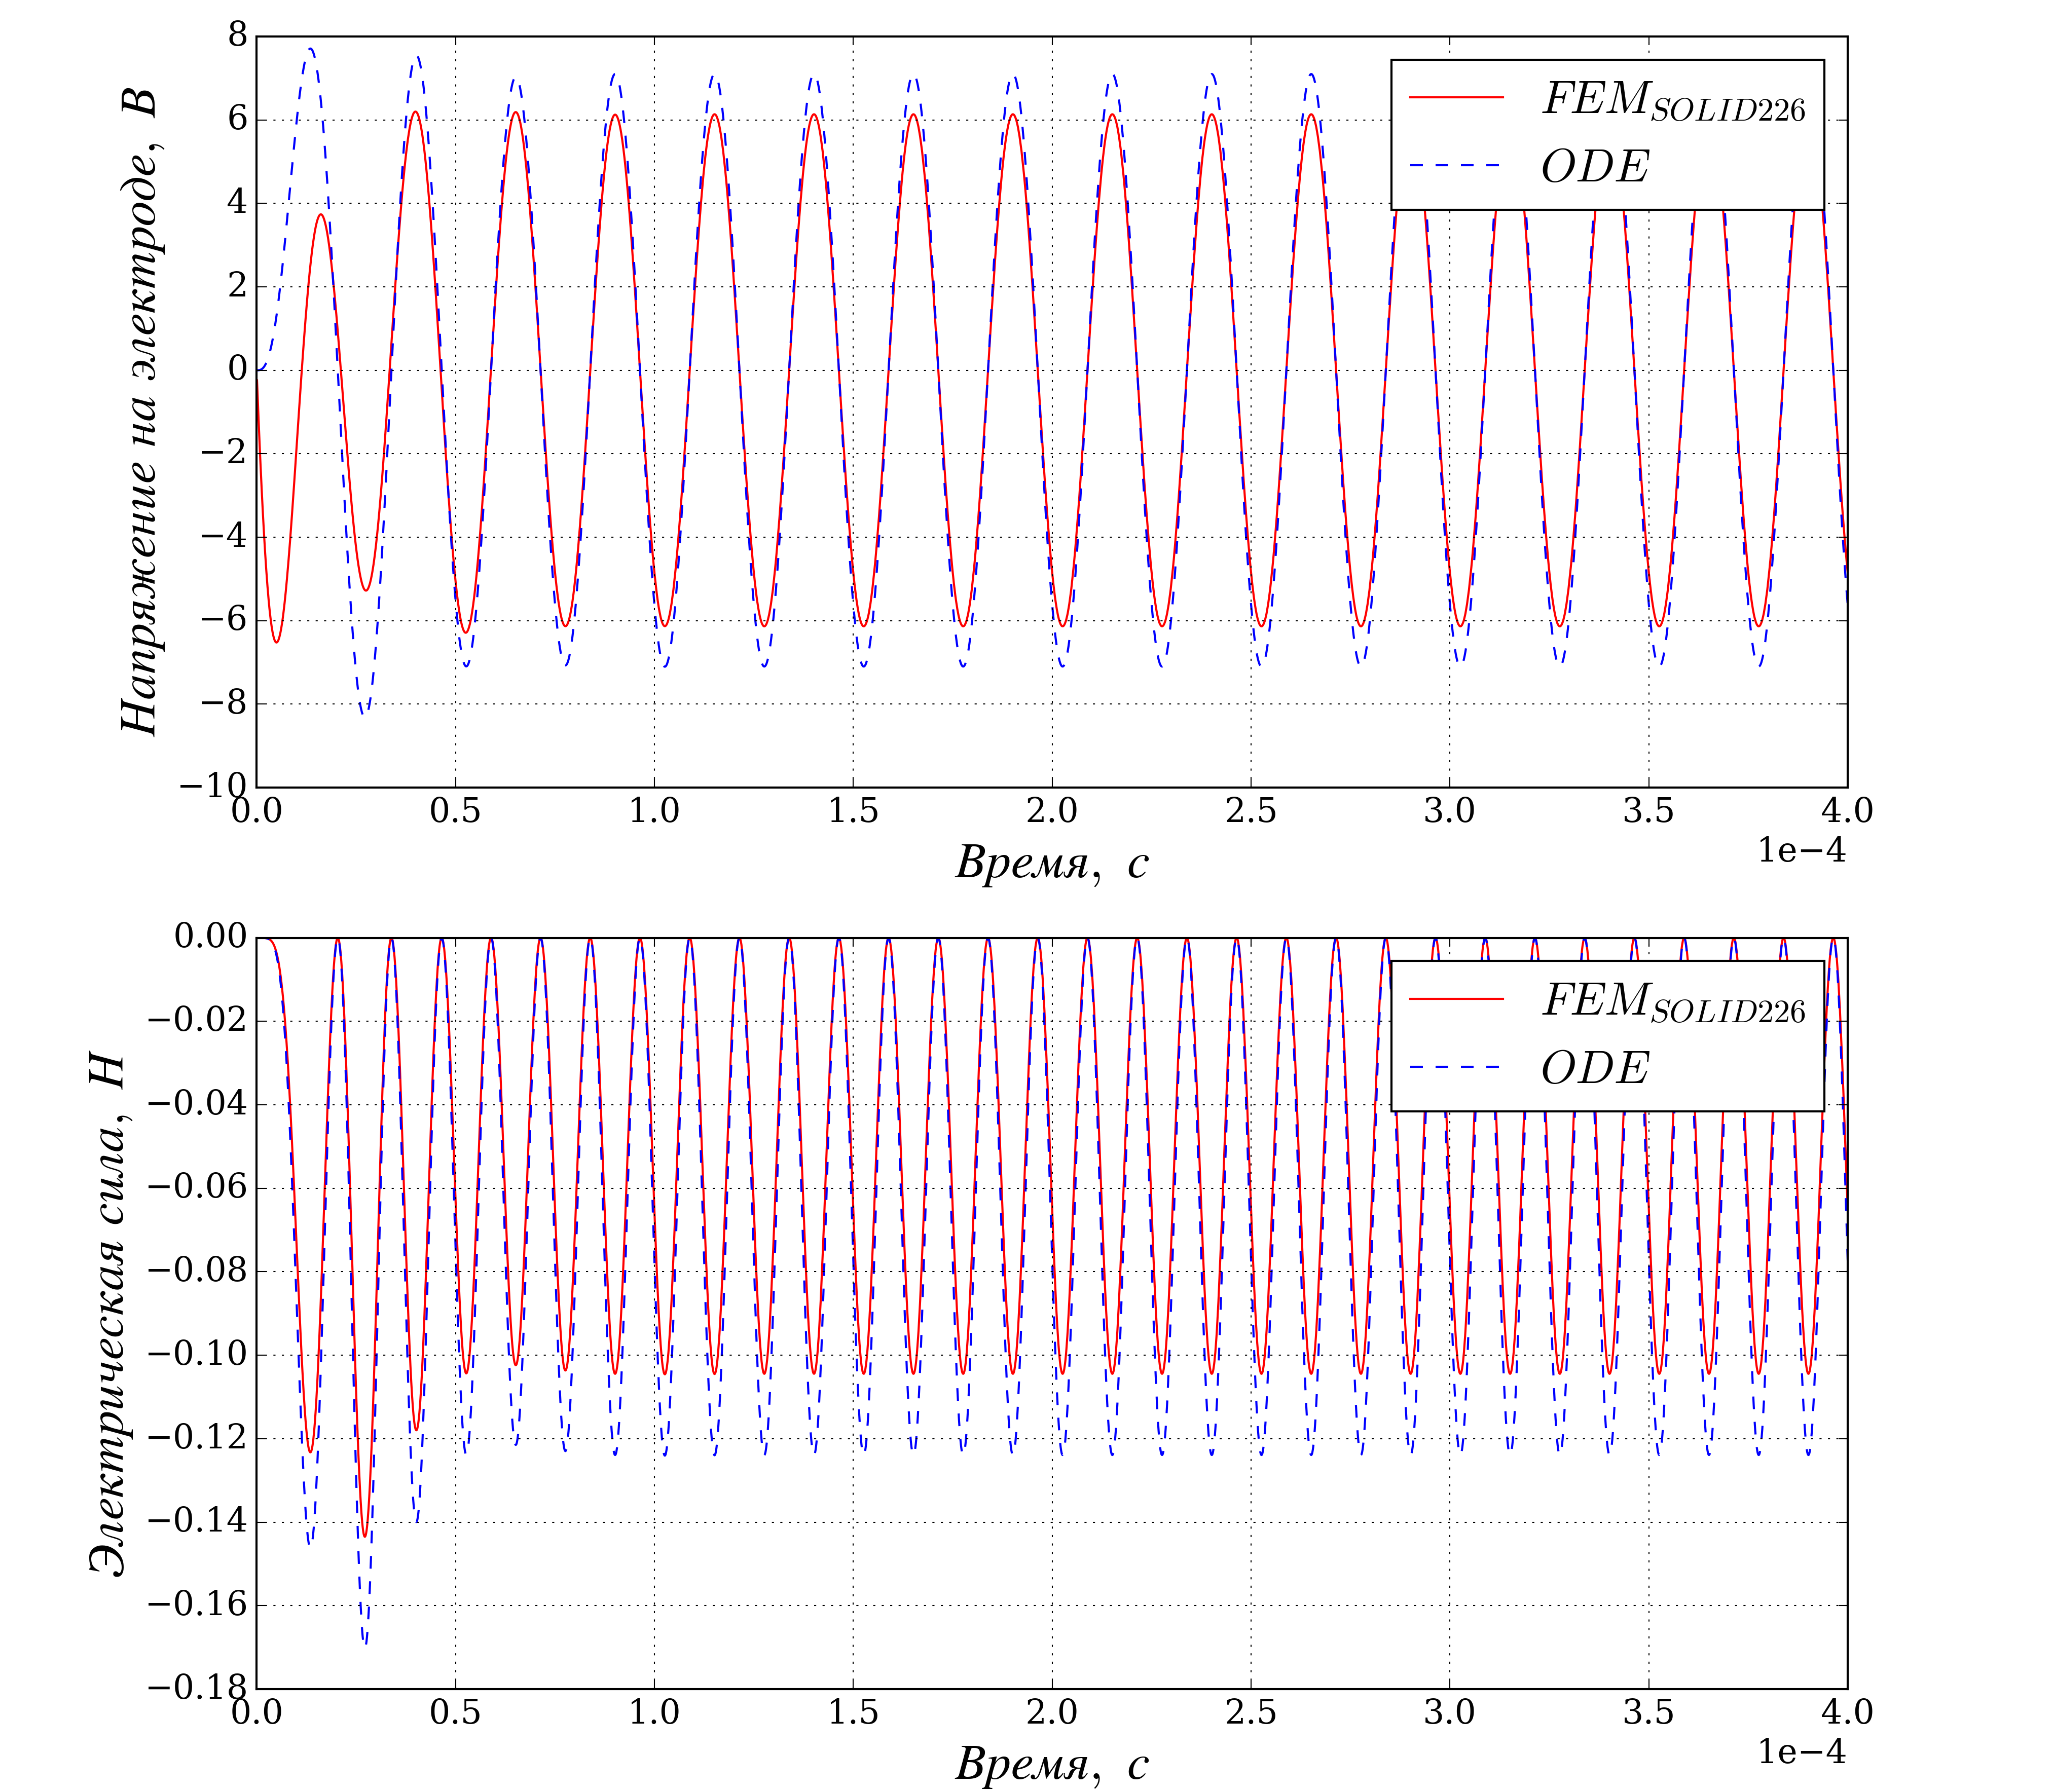
\includegraphics [scale=0.5] {pas_susp_solid226_sol}
  \caption{Результат конечно-элементного расчета методом прямого решения связанной задачи с фиксированным твердом телом в сравнении с численным решением ОДУ (\ref{eq:pas_susp_motion})}
  \label{img:pas_susp_solid226_sol}
\end{figure}

Метод прямого решения связанной задачи требует большого времени счета, что не позволяет выгодно применить его к расчету электромеханической задачи пассивного подвеса со сложной, с точки зрения геометрии, конечно-элементной сетки межэлектродной полостью: зазором $\delta_0 = 3\ \text{мкм}$ при площади $S = 50\ \text{см}^2$. Однако, это не исключает возможности его применения к более простым случаям, более того, метод, как упоминалось ранее, позволяет учитывать неоднородности электрического поля и при этом прост в реализации, что выгодно выделяет его на фоне других подходов.

По этой причине реализуем конечно-элементное решение задачи одноосного пассивного электростатического подвеса с помощью элементов-преобразователей, описанных ранее в разделе \ref{subsect2_2_2}.
Расчетную модель построим путем замыкания в контур 3-х элементов электрической цепи \textit{CIRCU124} и одного электромеханического \textit{TRANS126} элемента. Массу твердого тела, находящегося в пассивном электростатическом подвесе, моделируем \textit{MASS21} элементом. На верхний узел TRANS126, соответствующий верхнему фиксированному электроду, накладываем запрет на перемещение UY $= 0$. На нижний узел накладываем граничное условие первого рода VOLT $= 0$.

\begin{figure}[ht] 
  \centering
  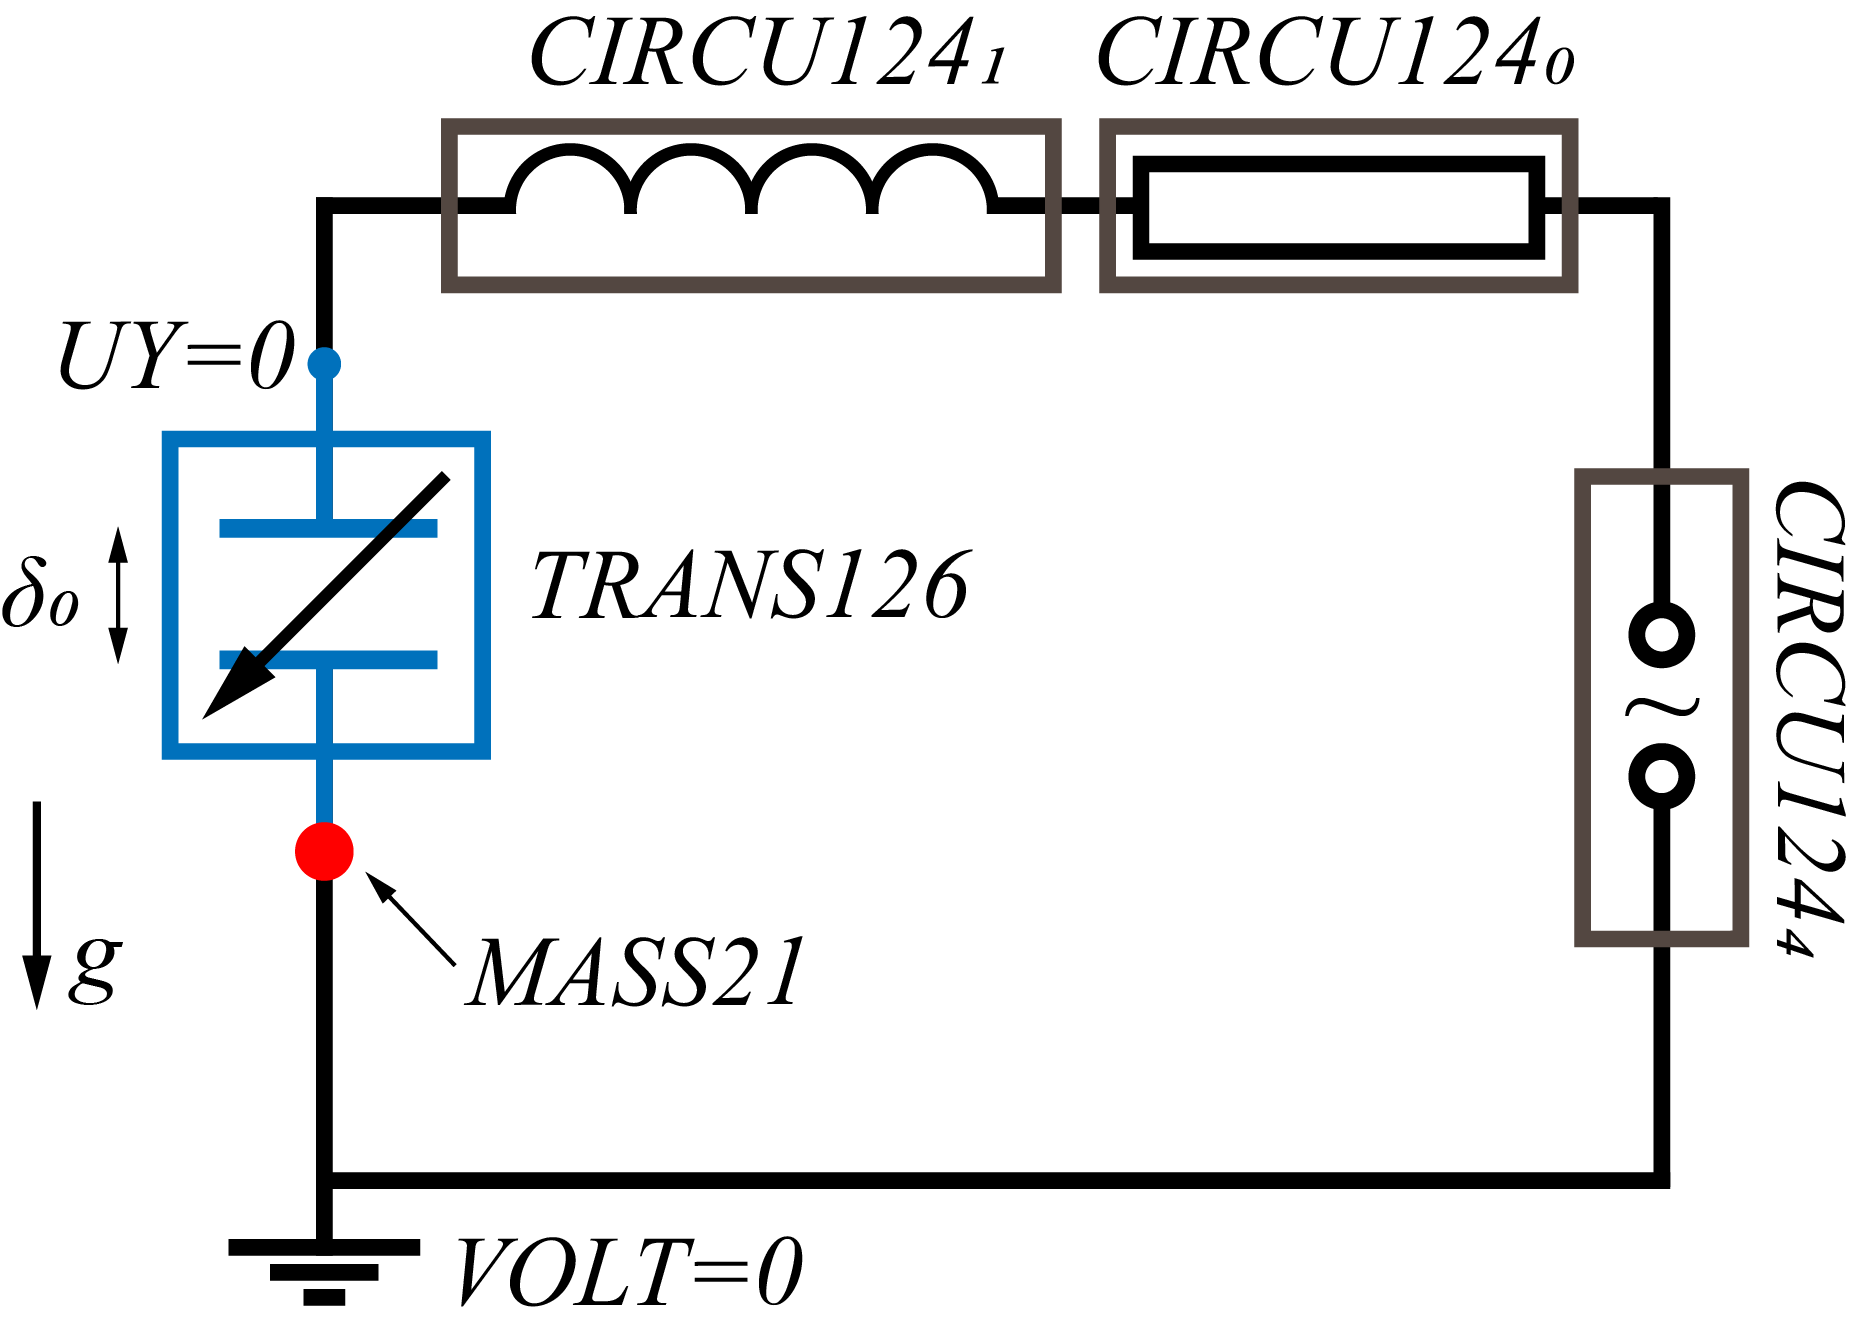
\includegraphics [scale=0.5] {pas_susp_trans126_scheme}
  \caption{Расчетная схема конечно-элементной постановки с использованием электромеханических элементов-преобразователей \textit{TRANS126}}
  \label{img:pas_susp_trans126_scheme}
\end{figure}


Как упоминалось ранее, для функционирования электромеханических элементов \textit{TRANS126} необходимо задание в них зависимости электрической емкости от зазора $C(\delta)$, где $\delta = \delta_0 + y_1 - y_2$, $\delta_0$ – номинальный зазор, $y_1, y_2$ – координаты первого и второго узлов элемента. Для расчета электрической емкости используем макрос \textit{CMATRIX}, позволяющий вычислить емкость между двумя фиксированными электродами. Для этого построим конечно-элементную модель эквивалентную конденсатору с площадью обкладок каждого электрода $S = 50\ \text{см}^2$. Для построения модели используем двумерные 8-ми узловые электростатические элементы \textit{PLANE121} с одной степенью свободы VOLT в каждом узле.

Итерационно в 20 шагов (именно столько точек на зависимости «зазор–емкость» способен хранить элемент \textit{TRANS126}) перестраиваем расчетную модель, изменяя на каждом шаге зазор между обкладками, исследуем зависимость электрической емкости от зазора на промежутке $1\ \text{мкм} < \delta < 10\ \text{мкм}$, напомним, что номинальный зазор $\delta_0 = 3\ \text{мкм}$.


\begin{figure}[ht] 
  \centering
  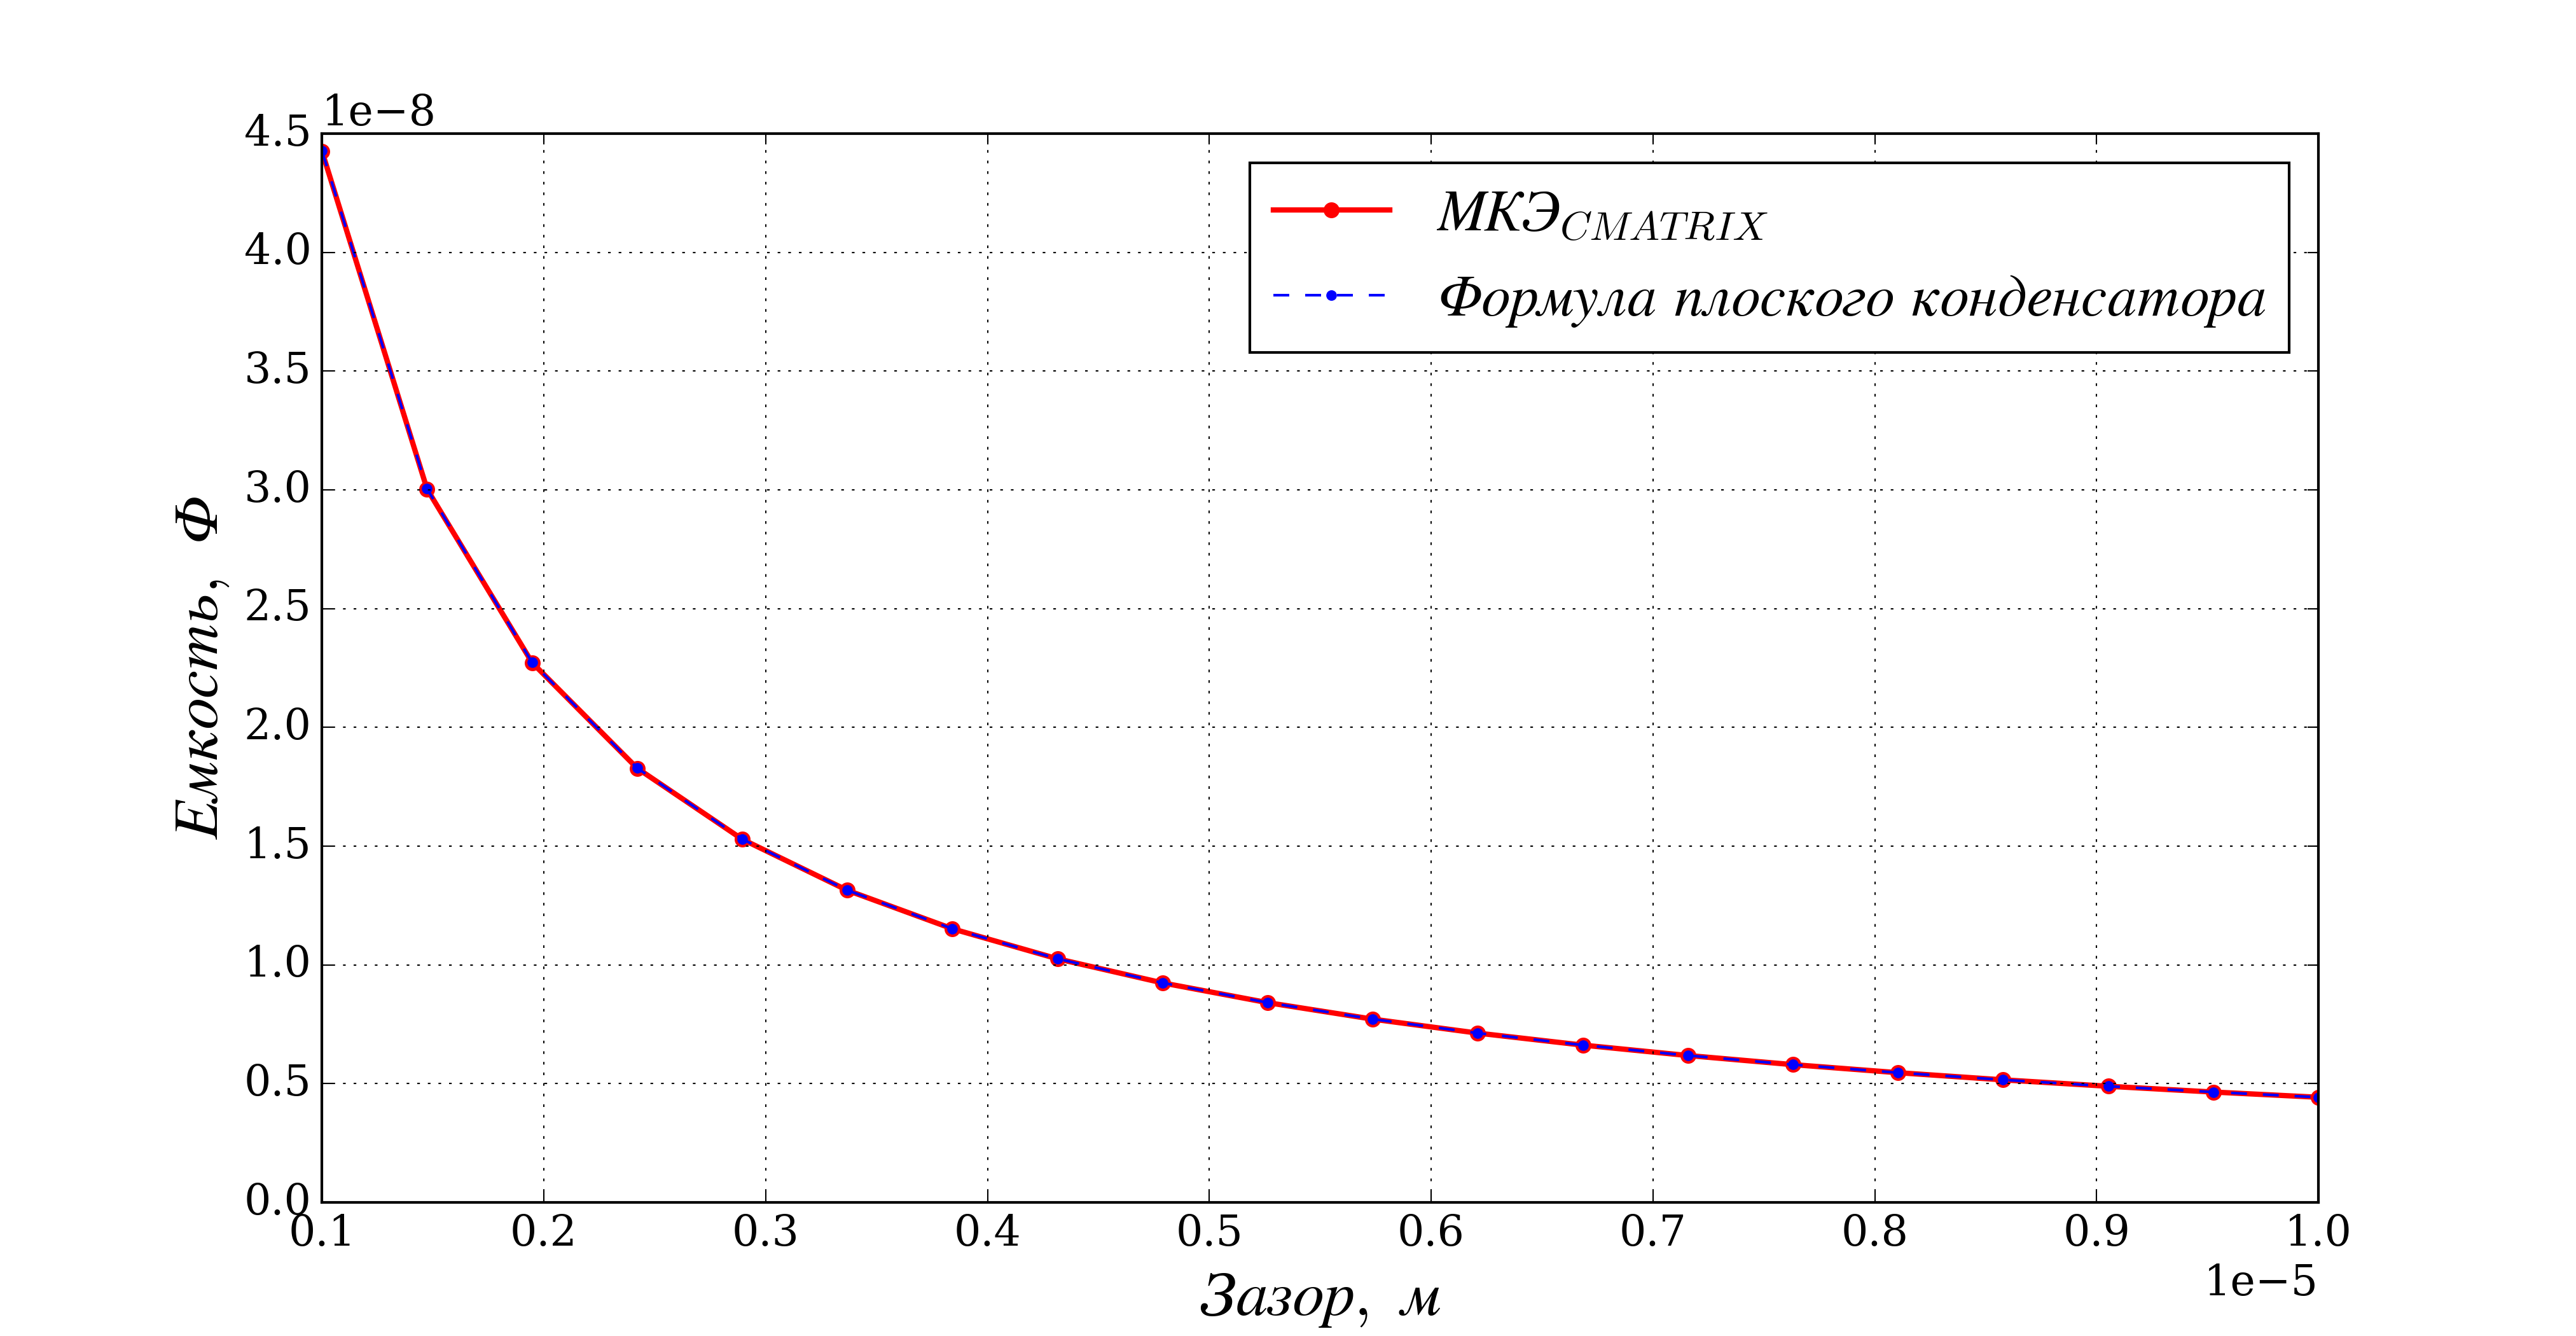
\includegraphics [scale=0.5] {pas_susp_trans126_cap_v_gap}
  \caption{График зависимости емкости от зазора $C(\delta)$, полученной методом конечных элементов, в сравнении с формулой емкости для плоского конденсатора}
  \label{img:pas_susp_trans126_cap_v_gap}
\end{figure}

Прежде чем производить динамический анализ убедимся в работоспособности пассивного подвеса с текущими параметрами, т.~е. в том, что в положении $y = \delta_0 = 3\ \text{мкм}$ с учетом допущений, сделанных в разделе \ref{subsect2_2_1}, пассивный подвес способен удерживать тело. Это условие выполнится, если зависимость пондеромоторной силы, действующей на тело в подвесе, от зазора будет иметь резонансный характер, т.~е. возрастать при отдалении тела от фиксированного электрода и убывать при его приближении к электроду. Построим график зависимости пондеромоторной электрической силы от зазора между фиксированным электродом  и твердым телом (рис. \ref{img:pas_susp_trans126_force_v_gap}).

Нетрудно видеть, что, как и на рис. \ref{img:active_susp_force_plot}, зависимость электрической силы от зазора на рис. \ref{img:pas_susp_trans126_force_v_gap} имеет резонансный характер. Точка пересечения графика силы с прямой силы тяжести $mg = 6.25\ \text{г} \cdot 9.8 \frac{\text{м}}{\text{с}^2}$ имеет абсциссу $3\ \text{мкм}$, а значит выбор параметров подвеса был осуществлен верно.


\begin{figure}[ht] 
  \centering
  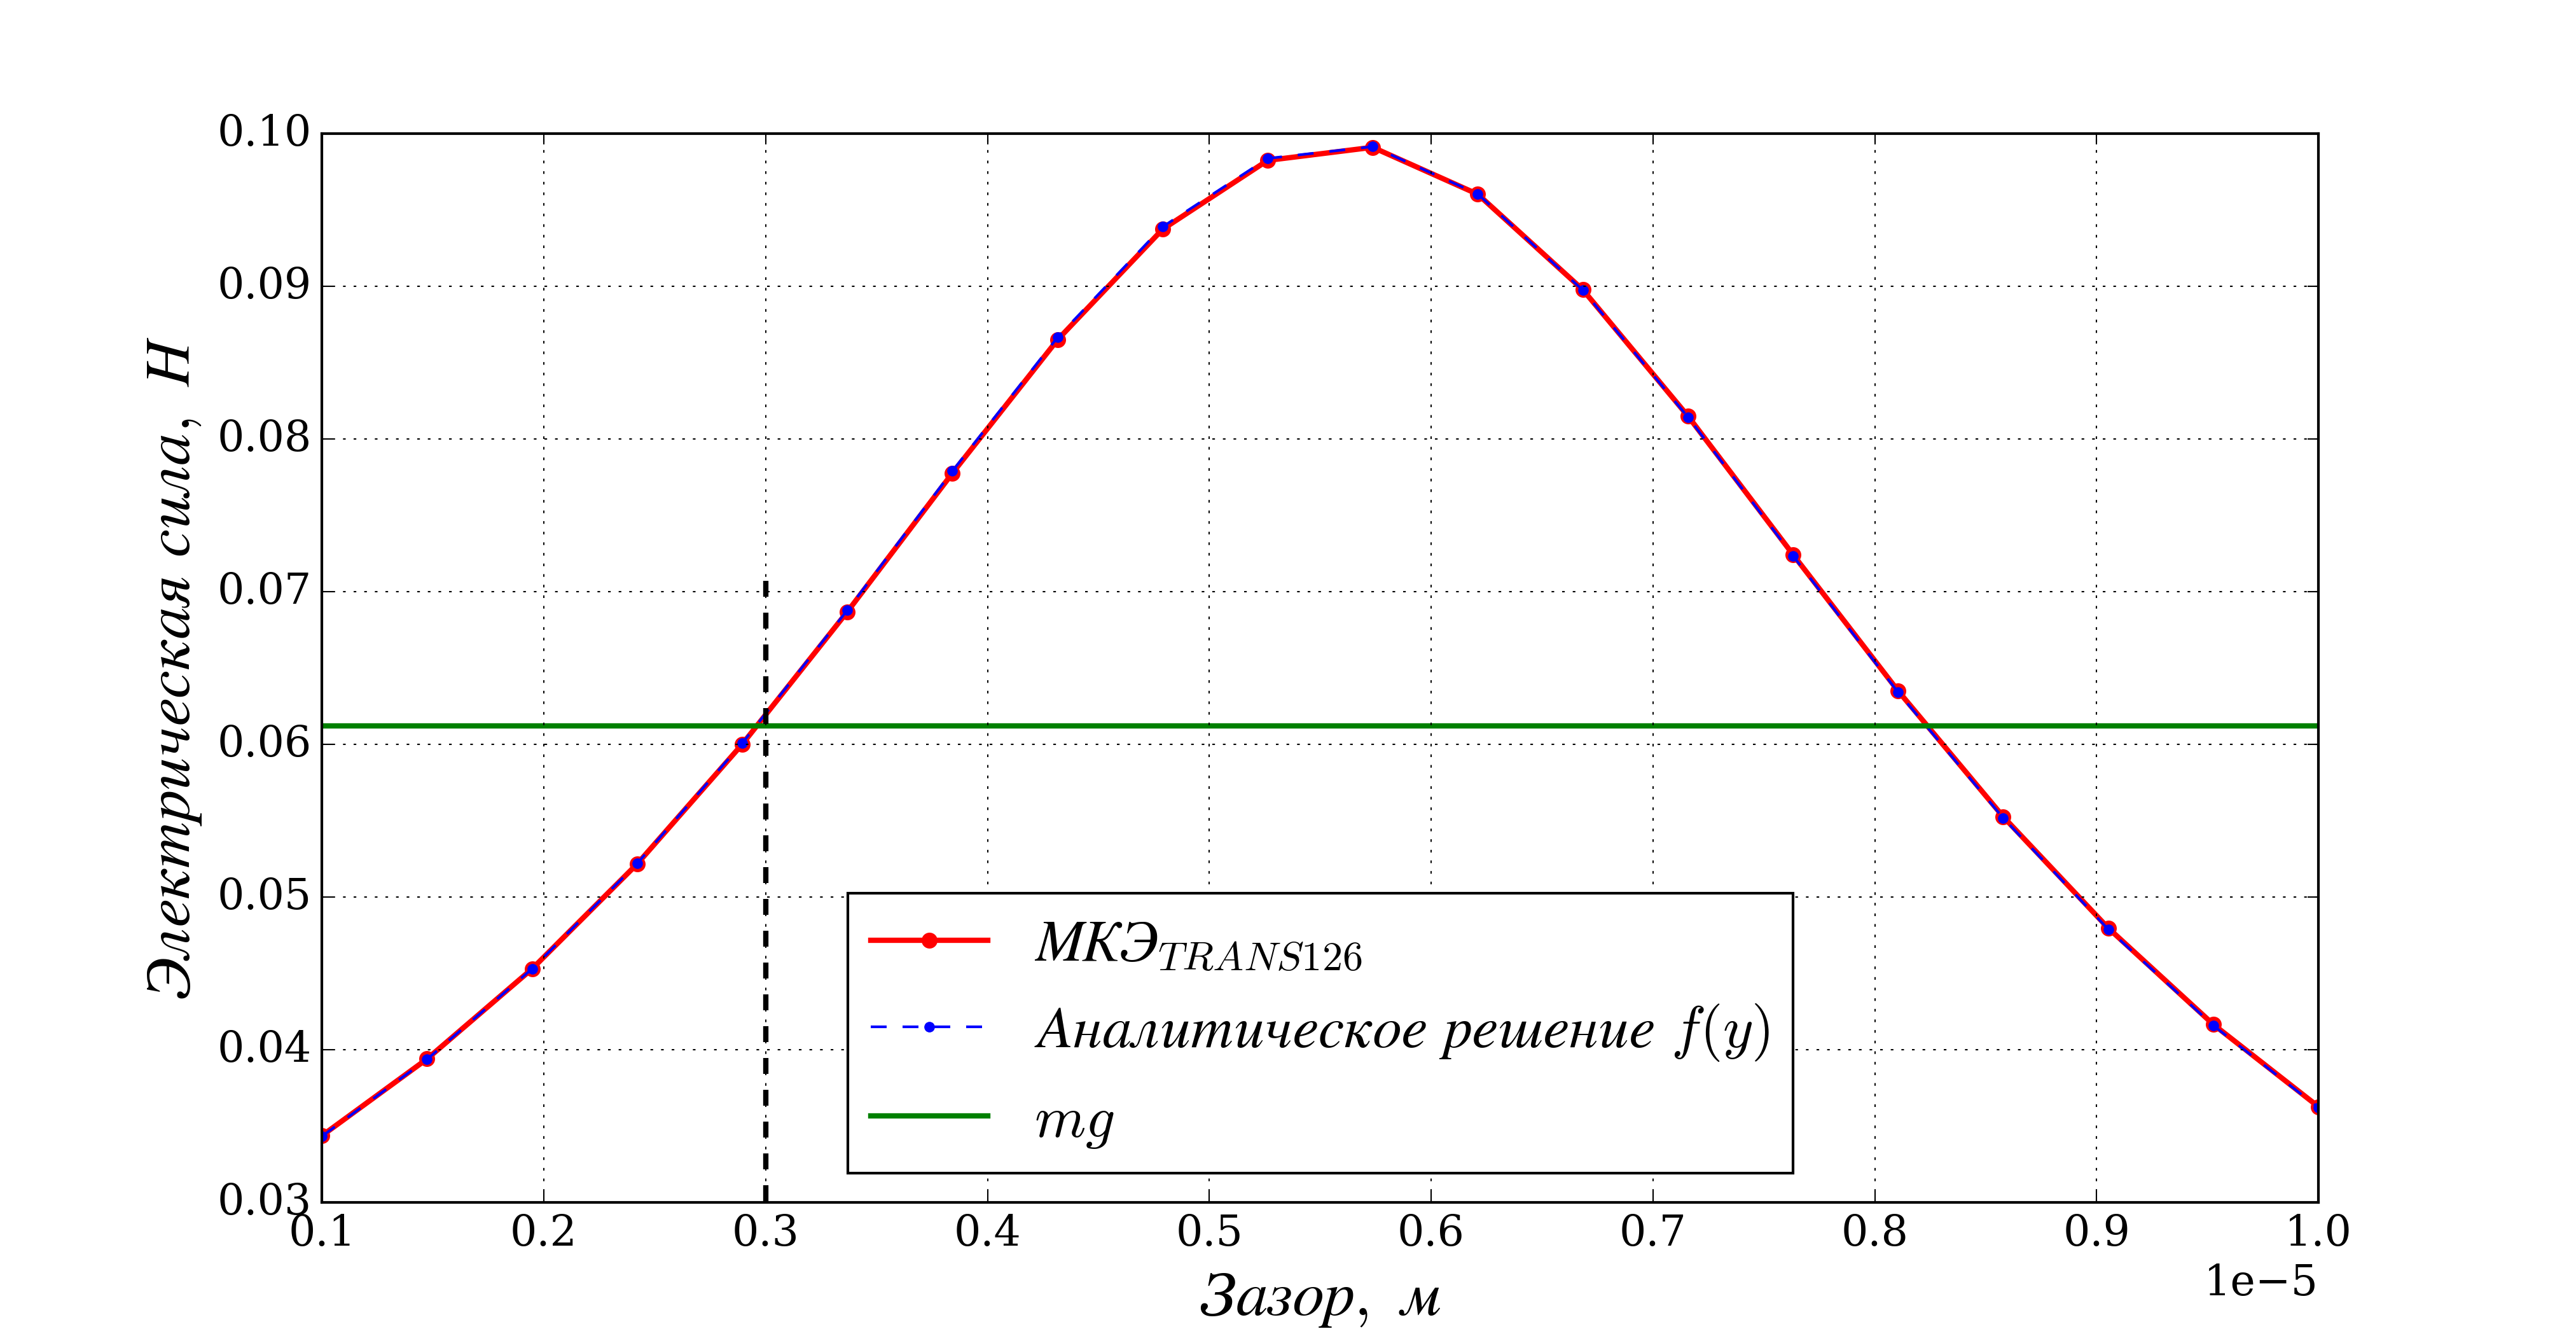
\includegraphics [scale=0.5] {pas_susp_trans126_force_v_gap}
  \caption{График зависимости емкости от зазора $C(\delta)$, полученной методом конечных элементов, в сравнении с формулой емкости для плоского конденсатора}
  \label{img:pas_susp_trans126_force_v_gap}
\end{figure}

Результаты динамического анализа конечно-элементной расчетной модели подвеса методом Ньютона-Рафсона представлены далее в разделе \ref{sect2_3_1}. Прежде, убедимся в сходимости численного конечно-элементного решения, построив график зависимости вертикальной координаты твердого тела $y$ от количества шагов интегрирования на один период источника напряжения $T = 1/\omega$. График сходимости представлен на рис. \ref{img:pas_susp_trans126_conv}. Исходя из результата, выберем шаг интегрирования $dt_{max}=\frac{1}{32} \cdot T$.
 
\begin{figure}[ht] 
  \centering
  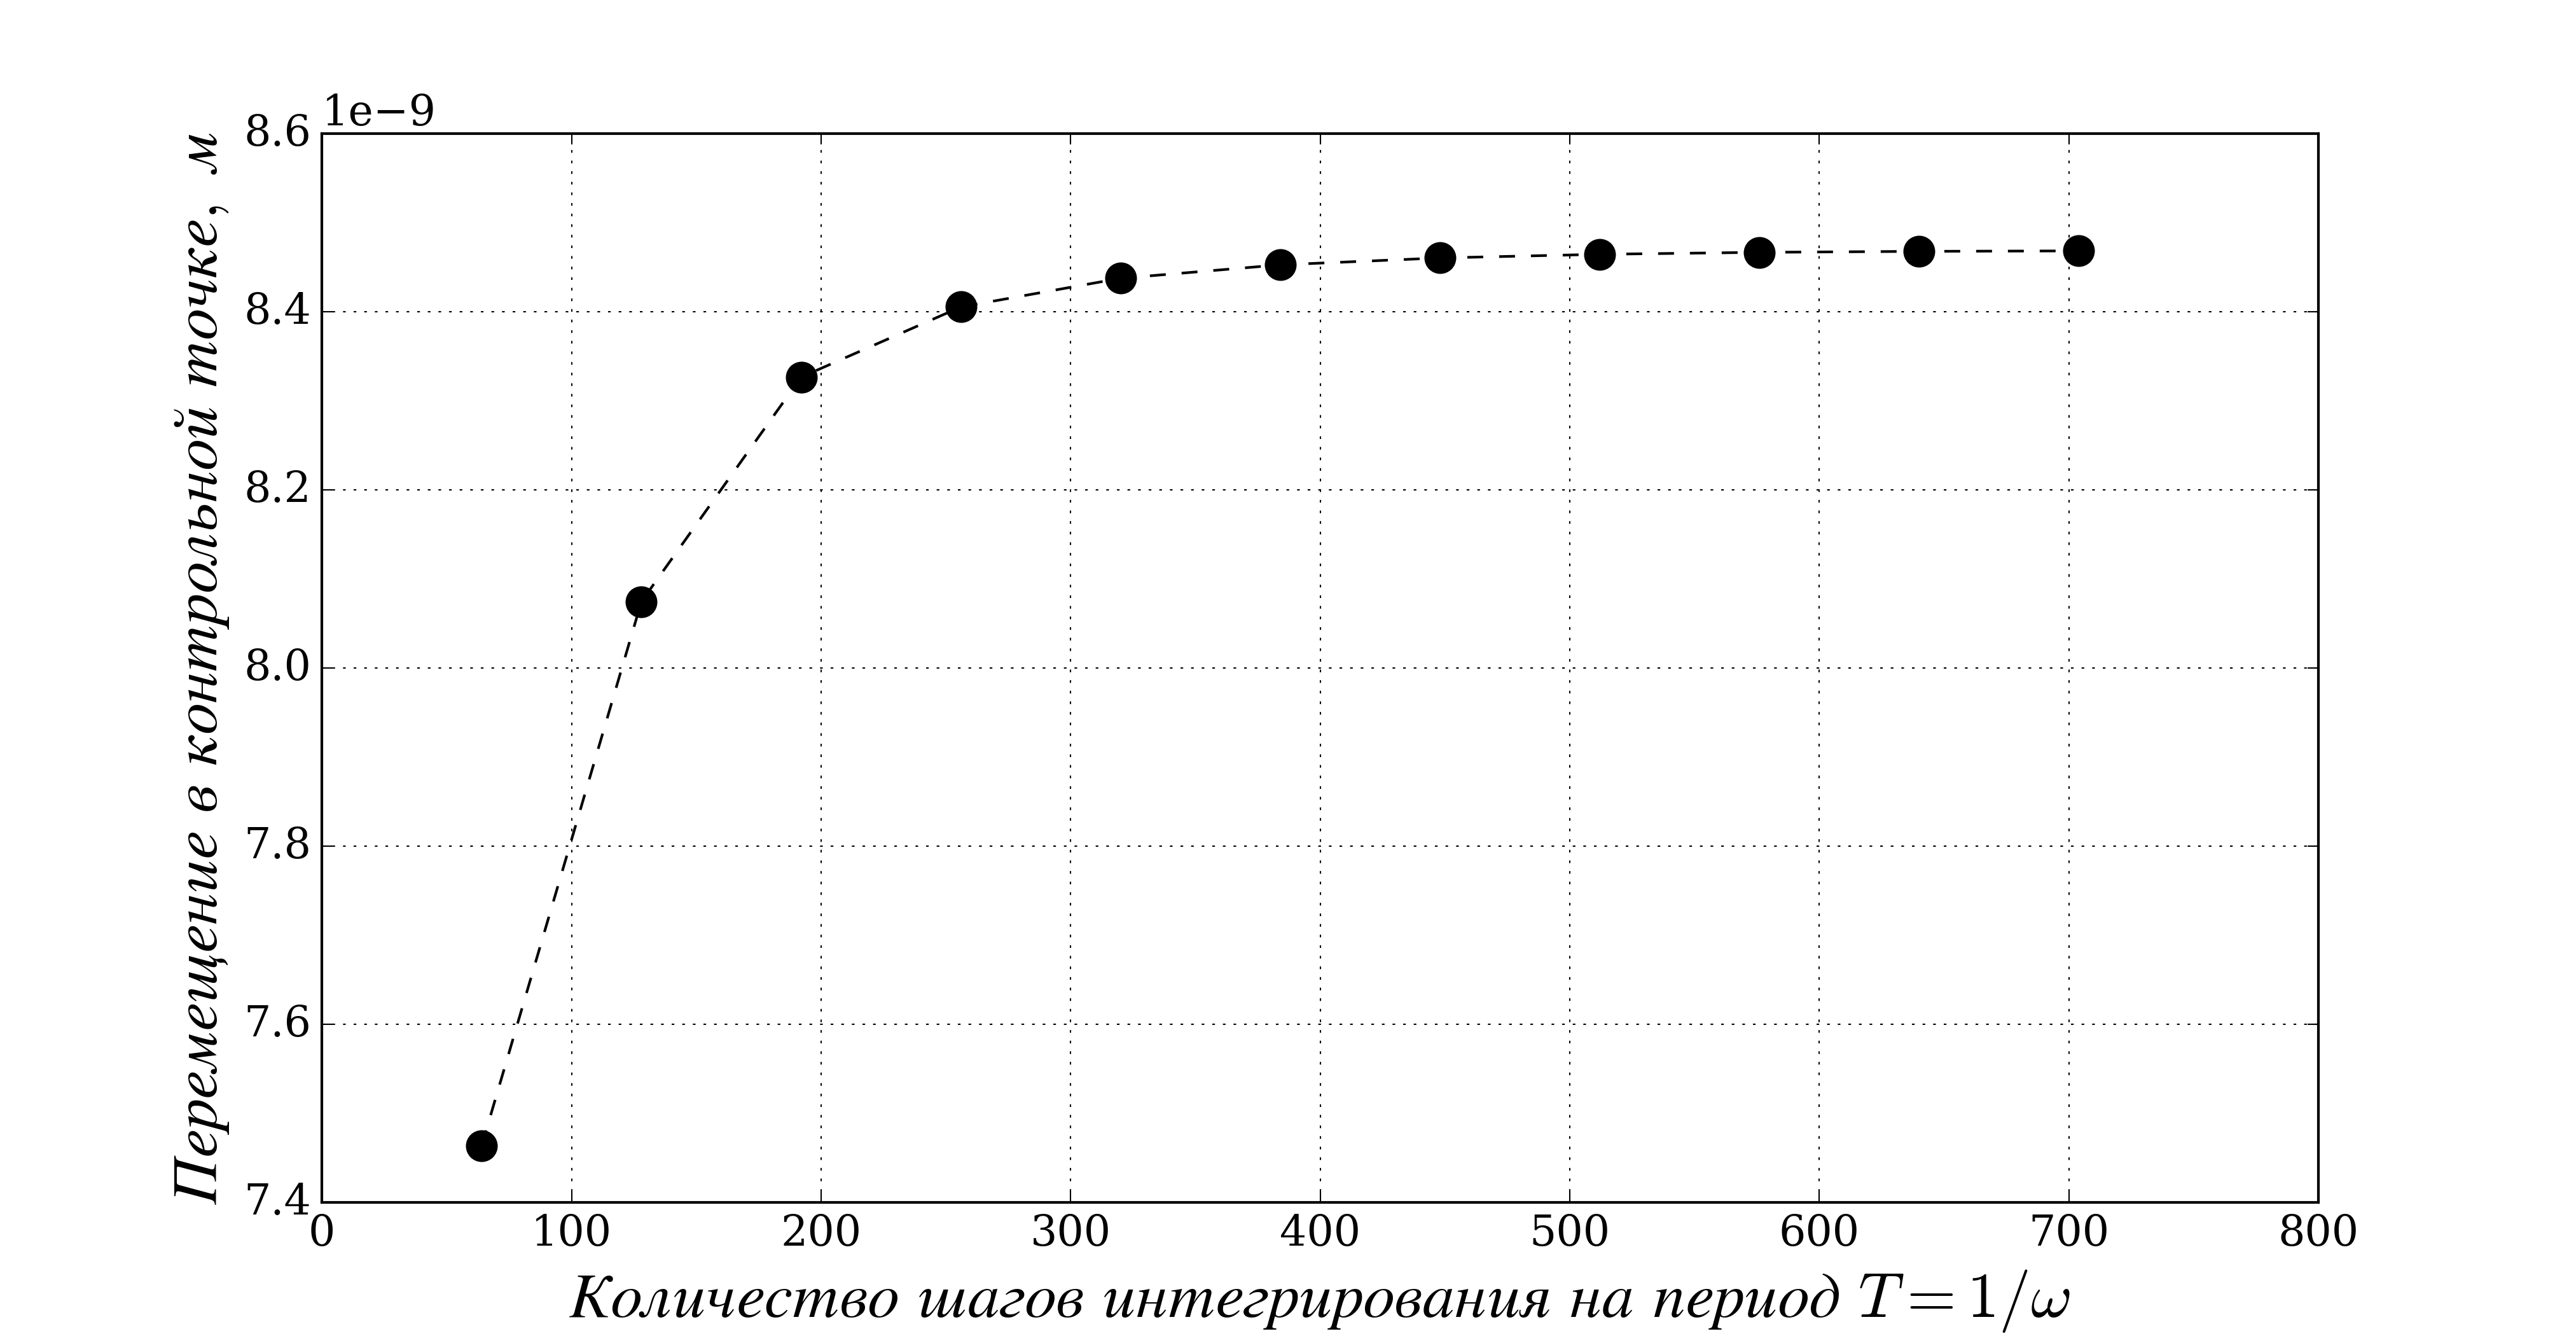
\includegraphics [scale=0.5] {pas_susp_trans126_conv}
  \caption{График сходимости численного конечно-элементного решения в модели с электромеханическим элементом \textit{TRANS126}}
  \label{img:pas_susp_trans126_conv}
\end{figure}


%\newpage
%============================================================================================================================
\section{Анализ полученных уравнений методом многих масштабов} \label{sect2_3}

Ранее были получены аналитические оценки поведения решения системы уравнений (\ref{eq:pas_susp_motion}). Уравнение (\ref{eq:pas_susp_sol_1}) получено с нестрогим допущением, что частота источника напряжения $\omega$ много больше частоты механических колебаний твердого тела. Для оценки корректности введенного допущения построим асимптотическое решение системы (\ref{eq:pas_susp_motion}) в нулевом и первом приближениях. 


\section{Сравнение результатов в задаче динамики одномерного электрического подвеса с явным моделированием связной задачи в ANSYS} \label{sect2_3_1}


% \begin{figure}[ht] 
%   \centering
%   \includegraphics [scale=0.5] {pas_susp_trans126_sol}
%   \caption{Результат конечно-элементного расчета методом прямого решения связанной задачи с фиксированным твердом телом в сравнении с численным решением ОДУ (\ref{eq:pas_susp_motion})}
%   \label{img:pas_susp_trans126_sol}
% \end{figure}


           % Глава 2
\chapter{Сферический пассивный электростатический подвес} \label{chapt3}

\section{Определение главного вектора сил и главного момента для сферического тела в электростатическом подвесе} \label{sect3_1}

\section{Анализ жесткости электростатического подвеса для различной формы электродов}\label{sect3_2}

           % Глава 3
% \chapter{Электростатический подвес} \label{chapt4}

\section{Обзор технических элементов, в которых находит свое применение электростатический подвес} \label{sect4_1}


%\newpage
%============================================================================================================================

\section{Обоснованность применения теории электростатики} \label{sect4_2}

           % Глава 4
\chapter*{Заключение}						% Заголовок
\addcontentsline{toc}{chapter}{Заключение}	% Добавляем его в оглавление

%% Согласно ГОСТ Р 7.0.11-2011:
%% 5.3.3 В заключении диссертации излагают итоги выполненного исследования, рекомендации, перспективы дальнейшей разработки темы.
%% 9.2.3 В заключении автореферата диссертации излагают итоги данного исследования, рекомендации и перспективы дальнейшей разработки темы.
%% Поэтому имеет смысл сделать эту часть общей и загрузить из одного файла в автореферат и в диссертацию:

Основные результаты работы заключаются в следующем.
%% Согласно ГОСТ Р 7.0.11-2011:
%% 5.3.3 В заключении диссертации излагают итоги выполненного исследования, рекомендации, перспективы дальнейшей разработки темы.
%% 9.2.3 В заключении автореферата диссертации излагают итоги данного исследования, рекомендации и перспективы дальнейшей разработки темы.
\begin{enumerate}
  \item На основе анализа уравнений энергии одноосного подвеса была показана невозможность нахождения тела в положении устойчивого равновесия без управления напряжением.
  \item Исследована модель одноосного пассивного электростатического подвеса с переменным напряжением
  \item Описаны основные подходы при моделировании задач электромеханики в программной системе конечно-элементного анализа
  \item Произведено конечно-элементное моделирование задачи одноосного пассивного электростатического подвеса
  \item Произведен анализ и конечно-элементное моделирование задачи одноосного пассивного электростатического подвеса
  \item Произведено конечно-элементное моделирование задачи сферического трехосного пассивного электростатического подвеса
\end{enumerate}




В заключение автор
выражает благодарность и большую признательность научному руководителю
Попову~И.А. за поддержку, помощь, обсуждение результатов и научное
руководство.
      % Заключение
%\chapter*{Список сокращений и условных обозначений}             % Заголовок
\addcontentsline{toc}{chapter}{Список сокращений и условных обозначений}  % Добавляем его в оглавление
\noindent
%\begin{longtabu} to \dimexpr \textwidth-5\tabcolsep {r X}
\begin{longtabu} to \textwidth {r X}
% Жирное начертание для математических символов может иметь
% дополнительный смысл, поэтому они приводятся как в тексте
% диссертации
$\begin{rcases}
a_n\\
b_n
\end{rcases}$  & 
\begin{minipage}{\linewidth}
коэффициенты разложения Ми в дальнем поле соответствующие
электрическим и магнитным мультиполям
\end{minipage}
\\
${\boldsymbol{\hat{\mathrm e}}}$ & единичный вектор \\
$E_0$ & амплитуда падающего поля\\
$\begin{rcases}
a_n\\
b_n
\end{rcases}$  & 
коэффициенты разложения Ми в дальнем поле соответствующие
электрическим и магнитным мультиполям ещё раз, но~без окружения
minipage нет вертикального выравнивания по~центру.
\\
$j$ & тип функции Бесселя\\
$k$ & волновой вектор падающей волны\\

$\begin{rcases}
a_n\\
b_n
\end{rcases}$  & 
\begin{minipage}{\linewidth}
\vspace{0.7em}
и снова коэффициенты разложения Ми в дальнем поле соответствующие
электрическим и магнитным мультиполям, теперь окружение minipage есть
и добавлено много текста, так что описание группы условных
обозначений значительно превысило высоту этой группы... Для отбивки
пришлось добавить дополнительные отступы.
\vspace{0.5em}
\end{minipage}
\\
$L$ & общее число слоёв\\
$l$ & номер слоя внутри стратифицированной сферы\\
$\lambda$ & длина волны электромагнитного излучения
в вакууме\\
$n$ & порядок мультиполя\\
$\begin{rcases}
{\mathbf{N}}_{e1n}^{(j)}&{\mathbf{N}}_{o1n}^{(j)}\\
{\mathbf{M}_{o1n}^{(j)}}&{\mathbf{M}_{e1n}^{(j)}}
\end{rcases}$  & сферические векторные гармоники\\
$\mu$  & магнитная проницаемость в вакууме\\
$r,\theta,\phi$ & полярные координаты\\
$\omega$ & частота падающей волны\\

  \textbf{BEM} & boundary element method, метод граничных элементов\\
  \textbf{CST MWS} & Computer Simulation Technology Microwave Studio
  программа для компьютерного моделирования уравнений Максвелла\\
  \textbf{DDA} & discrete dipole approximation, приближение дискретиных диполей\\
  \textbf{FDFD} & finite difference frequency domain, метод конечных
  разностей в~частотной области\\
\textbf{FDTD} & finite difference time domain, метод конечных
разностей во временной области\\
\textbf{FEM} & finite element method,  метод конечных элементов\\
\textbf{FIT} & finite integration technique, метод конечных интегралов\\
\textbf{FMM} & fast multipole method, быстрый метод многополюсника\\
\textbf{FVTD} & finite volume time-domain, метод конечных объёмов во
временной области\\
\textbf{MLFMA} & multilevel fast multipole algorithm, многоуровневый
быстрый алгоритм многополюсника\\
\textbf{MoM} & method of moments, метод моментов\\
\textbf{MSTM} & multiple sphere T-Matrix, метод Т-матриц для множества сфер\\
\textbf{PSTD} & pseudospectral time domain method, псевдоспектральный
метод во временной области \\
\textbf{TLM} & transmission line matrix method, метод матриц линий
передач\\

\end{longtabu}
\addtocounter{table}{-1}% Нужно откатить на единицу счетчик номеров таблиц, так как предыдующая таблица сделана для удобства представления информации по ГОСТ
        % Список сокращений и условных обозначений
%\chapter*{Словарь терминов}             % Заголовок
\addcontentsline{toc}{chapter}{Словарь терминов}  % Добавляем его в оглавление

\textbf{TeX} - Cистема компьютерной вёрстки, разработанная американским профессором информатики Дональдом Кнутом

\textbf{Панграмма} - Короткий текст, использующий все или почти все буквы алфавита
      % Словарь терминов
\clearpage                                  % В том числе гарантирует, что список литературы в оглавлении будет с правильным номером страницы
%\hypersetup{ urlcolor=black }               % Ссылки делаем чёрными
%\providecommand*{\BibDash}{}                % В стилях ugost2008 отключаем использование тире как разделителя 
\urlstyle{rm}                               % ссылки URL обычным шрифтом
\ifdefmacro{\microtypesetup}{\microtypesetup{protrusion=false}}{} % не рекомендуется применять пакет микротипографики к автоматически генерируемому списку литературы
\insertbibliofull                           % Подключаем Bib-базы
\ifdefmacro{\microtypesetup}{\microtypesetup{protrusion=true}}{}
\urlstyle{tt}                               % возвращаем установки шрифта ссылок URL
%\hypersetup{ urlcolor={urlcolor} }          % Восстанавливаем цвет ссылок      % Список литературы
%\clearpage
\ifdefmacro{\microtypesetup}{\microtypesetup{protrusion=false}}{} % не рекомендуется применять пакет микротипографики к автоматически генерируемым спискам
\listoffigures  % Список изображений

%%% Список таблиц %%%
% (ГОСТ Р 7.0.11-2011, 5.3.10)
\clearpage
\listoftables   % Список таблиц
\ifdefmacro{\microtypesetup}{\microtypesetup{protrusion=true}}{}
\newpage           % Списки таблиц и изображений (иллюстративный материал)
% \appendix
%%% Оформление заголовков приложений ближе к ГОСТ:
\setlength{\midchapskip}{20pt}
\renewcommand*{\afterchapternum}{\par\nobreak\vskip \midchapskip}
\renewcommand\thechapter{\Asbuk{chapter}} % Чтобы приложения русскими буквами нумеровались
   % Предварительные настройки для правильного подключения Приложений
\chapter{Листинги программного кода APDL} \label{AppendixA}

Для крупных листингов есть два способа. Первый красивый, но в нём могут быть проблемы с поддержкой кириллицы (у вас может встречаться в комментариях и
печатаемых сообщениях), он представлен на листинге~\ref{list:hwbeauty}.
\begin{ListingEnv}[!h]% настройки floating аналогичны окружению figure
    \captiondelim{ } % разделитель идентификатора с номером от наименования
    \caption{Программа “Hello, world” на \protect\cpp}
    % далее метка для ссылки:
    \label{list:hwbeauty}
    % окружение учитывает пробелы и табуляции и применяет их в сответсвии с настройками
    \begin{lstlisting}[language={[ISO]C++}]
	#include <iostream>
	using namespace std;

	int main() //кириллица в комментариях при xelatex и lualatex имеет проблемы с пробелами
	{
		cout << "Hello, world" << endl; //latin letters in commentaries
		system("pause");
		return 0;
	}
    \end{lstlisting}
\end{ListingEnv}%
Второй не такой красивый, но без ограничений (см.~листинг~\ref{list:hwplain}).
\begin{ListingEnv}[!h]
    \captiondelim{ } % разделитель идентификатора с номером от наименования
    \caption{Программа “Hello, world” без подсветки}
    \label{list:hwplain}
    \begin{Verb}
        
        #include <iostream>
        using namespace std;
        
        int main() //кириллица в комментариях
        {
            cout << "Привет, мир" << endl;
        }
    \end{Verb}
\end{ListingEnv}

Можно использовать первый для вставки небольших фрагментов
внутри текста, а второй для вставки полного
кода в приложении, если таковое имеется.

Если нужно вставить совсем короткий пример кода (одна или две строки), то выделение  линейками и нумерация может смотреться чересчур громоздко. В таких случаях можно использовать окружения \texttt{lstlisting} или \texttt{Verb} без \texttt{ListingEnv}. Приведём такой пример с указанием языка программирования, отличного от заданного по умолчанию:
\begin{lstlisting}[language=Haskell]
fibs = 0 : 1 : zipWith (+) fibs (tail fibs)
\end{lstlisting}
Такое решение~--- со вставкой нумерованных листингов покрупнее
и вставок без выделения для маленьких фрагментов~--- выбрано,
например, в книге Эндрю Таненбаума и Тодда Остина по архитектуре
%компьютера~\autocite{TanAus2013} (см.~рис.~\ref{fig:tan-aus}).

Наконец, для оформления идентификаторов внутри строк
(функция \lstinline{main} и~тому подобное) используется
\texttt{lstinline} или, самое простое, моноширинный текст
(\texttt{\textbackslash texttt}).


Пример~\ref{list:internal3}, иллюстрирующий подключение переопределённого языка. Может быть полезным, если подсветка кода работает криво. Без дополнительного окружения, с подписью и ссылкой, реализованной встроенным средством.
\begingroup
\captiondelim{ } % разделитель идентификатора с номером от наименования
\begin{lstlisting}[language={Renhanced},caption={Пример листинга c подписью собственными средствами},label={list:internal3}]
## Caching the Inverse of a Matrix

## Matrix inversion is usually a costly computation and there may be some
## benefit to caching the inverse of a matrix rather than compute it repeatedly
## This is a pair of functions that cache the inverse of a matrix.

## makeCacheMatrix creates a special "matrix" object that can cache its inverse

makeCacheMatrix <- function(x = matrix()) {#кириллица в комментариях при xelatex и lualatex имеет проблемы с пробелами
    i <- NULL
    set <- function(y) {
        x <<- y
        i <<- NULL
    }
    get <- function() x
    setSolved <- function(solve) i <<- solve
    getSolved <- function() i
    list(set = set, get = get,
    setSolved = setSolved,
    getSolved = getSolved)
    
}


## cacheSolve computes the inverse of the special "matrix" returned by
## makeCacheMatrix above. If the inverse has already been calculated (and the
## matrix has not changed), then the cachesolve should retrieve the inverse from
## the cache.

cacheSolve <- function(x, ...) {
    ## Return a matrix that is the inverse of 'x'
    i <- x$getSolved()
    if(!is.null(i)) {
        message("getting cached data")
        return(i)
    }
    data <- x$get()
    i <- solve(data, ...)
    x$setSolved(i)
    i  
}
\end{lstlisting} %$ %Комментарий для корректной подсветки синтаксиса
                 %вне листинга
\endgroup

Листинг~\ref{list:external1} подгружается из внешнего файла. Приходится загружать без окружения дополнительного. Иначе по страницам не переносится.
\begingroup
\captiondelim{ } % разделитель идентификатора с номером от наименования
    \lstinputlisting[lastline=300,language={Fortran},caption={Листинг из внешнего файла},label={list:external1}]{listings/suspension_3D.apdl}
\endgroup        % Приложения

\end{document}
